\author{Nguyễn Quốc Dương, Lê Phương Thảo, Đinh Thị Quỳnh Như, Cao Thị Ái Loan, Phùng Thị Hồng Diễm, GVHD: TS. Lê Thanh Bính.}
\documentclass[12pt, a4paper,oneside]{book}
\usepackage{amsmath, amssymb, latexsym, amscd, amsthm,amstext}
\usepackage{graphics}
\usepackage{color, colortbl}            % Màu trong bảng
\usepackage{varwidth}               

                          
\usepackage{hyperref}    
\usepackage[utf8]{vietnam}
\usepackage{anysize}							
\marginsize{3cm}{2cm}{2cm}{2cm}				%\marginsize{left}{right}{top}{bottom}
%\papersize{width}{height}	
\usepackage{listings}
\usepackage{booktabs}
\usepackage{siunitx}
\usepackage{longtable}                  % Tạo bảng dài
\usepackage{tocbibind}
\usepackage[toc,page]{appendix}         % Tô màu khung - nền - chữ
\usepackage{graphicx}
\usepackage{longfbox}		          	% Tạo hộp văn bản - box	
\title{Sections and Chapters}
\usepackage{multicol}
\usepackage{wrapfig}  
\usepackage{enumerate}
\usepackage{dsfont}
\usepackage{commath}
\renewcommand{\baselinestretch}{1.3} 
\renewcommand{\figurename}{\bf Hình}
%%========================================
\newtheorem{theo}{\bf Định lý}[section]
\newtheorem{coro}[theo]{\bf Corollary}
\newtheorem{lemm}[theo]{\bf Bổ đề}
\newtheorem{prop}[theo]{\bf Mệnh đề}
\newtheorem{algo}[theo]{\bf Thuật toán}
\newtheorem{conj}[theo]{\bf Conjecture}

\theoremstyle{definition}
\newtheorem{dn}[theo]{Định nghĩa}
\newtheorem{dl}[theo]{Định lý}
\newtheorem{tc}[theo]{Tính chất}
\newtheorem{vd}[theo]{\it Ví dụ}
\newtheorem{cy}[theo]{\it Chú ý}
\newtheorem{nx}[theo]{\it Nhận xét}
\newtheorem{pt}{\it Phân tích}
%\def\R{\mathbb{ R}}                        %Các kí hiệu tập hợp
%\def\re{\mbox{\rm \texttt{Re}}}            %Định nghĩa từ viết tắt
%\def\im{\mbox{\rm \texttt{Im}}}
%=========================================

\newcommand{\seq}[1]{\left<#1\right>}
\makeatletter
\def\ps@myheadings{%
	\def\@evenhead{\hfil\thepage\hfil}
	\def\@oddhead{\hfil\thepage\hfil}}
\makeatother 
\marginsize{3cm}{2.5cm}{2cm}{2cm}
\marginsize{3cm}{2.5cm}{2cm}{2cm}
\DeclareMathOperator{\sgn}{sgn}
\DeclareMathOperator{\rank}{rank}
\pagestyle{myheadings}
\newcommand{\blue}[1]{\textcolor{blue}{#1}}
\newcommand{\red}[1]{\textcolor{red}{#1}}
%=======================

\DeclareUnicodeCharacter{2212}{-}
\setlength{\parindent}{1 cm}
\usepackage{cases}
%=======================

\definecolor{dkgreen}{rgb}{0,0.6,0}             % Môi trường chứa code
\definecolor{gray}{rgb}{0.5,0.5,0.5}
\definecolor{mauve}{rgb}{0.58,0,0.82}
\lstset{frame=tb,
	language=R,
	aboveskip=3mm,
	belowskip=3mm,
	showstringspaces=false,
	columns=flexible,
	basicstyle={\small\ttfamily},
	numbers=none,
	numberstyle=\tiny\color{gray},
	keywordstyle=\color{blue},
	commentstyle=\color{dkgreen},
	stringstyle=\color{mauve},
	breaklines=true,
	breakatwhitespace=true,
	tabsize=3}
%=============================
\begin{document}
\tableofcontents
\newpage
\centerline{\bf THÔNG TIN KẾT QUẢ NGHIÊN CỨU CỦA ĐỀ TÀI}

\noindent 
{\bf 1. Thông tin chung:}

- Tên đề tài: \blue{Phân tích chuỗi thời gian bằng mô hình ARIMA với phần mềm R}

- Mã số: \textbf{S2019.564.01}

- Sinh viên thực hiện: - Cao Thị Ái Loan$^{1}$
                       
            \hspace{4cm}- Phùng Thị Hồng Diễm$^{1}$
            
            \hspace{4cm}- Nguyễn Quốc Dương$^{2}$
                       
            \hspace{4cm}- Lê Phương Thảo$^{2}$
            
            \hspace{4cm}- Đinh Thị Quỳnh Như$^{2}$
            
$^1$Lớp Toán học K39 Khoa: Toán và Thống kê\quad Năm thứ: 4\quad Số năm đào tạo: 4

$^2$Lớp Sư Phạm Toán K40 \quad Khoa: Sư Phạm \quad Năm thứ: 3\quad Số năm đào tạo: 4

- Người hướng dẫn: TS. Lê Thanh Bính

\noindent 
{\bf 2. Mục tiêu đề tài:}

- Nắm vững lý thuyết cơ bản về chuỗi thời gian và mô hình ARIMA; xây dựng quy trình dự báo bằng mô hình ARIMA gồm 5 bước sau: kiểm tra tính dừng của chuỗi thời gian; chuyển một chuỗi không dừng thành dừng; xác định bậc $p$, $q$, $P$, $Q$; kiểm tra độ chính xác của mô hình; bước cuối cùng là, dự báo.

- Nắm vững quy trình xây dựng mô hình ARIMA (với 5 bước nêu trên) bằng phần mềm R cho các dữ liệu thời gian thực trong những lĩnh vực khác nhau như khí tượng thủy văn; dịch tễ học; giáo dục; tài chính; chứng khoán.

\noindent 
{\bf 3. Tính mới và sáng tạo:} Áp dụng mô hình ARIMA để nghiên cứu độc lập trên các tập dữ liệu thực tế, ứng dụng trực tiếp cho địa phương và dự báo dịch bệnh COVID-19. Hơn nữa, chúng tôi so sánh khả năng dự báo của mô hình ARIMA với NNAR để có cái nhìn khách quan hơn.

\noindent 
{\bf 4. Kết quả nghiên cứu:}
Phân tích tổng quan tình hình COVID-19 trên toàn thế giới, phân tích và dự báo số ca nhiễm mới COVID-19 tại Mỹ và số ca tử vong mới COVID-19 tại Italy, dự báo lượng mưa tại trạm quan trắc Quy Nhơn và tạo một website Dashboard COVID-19 để theo dõi xu hướng dịch bệnh bằng mô hình ARIMA.
 
\noindent 
{\bf 5. Đóng góp về mặt kinh tế-xã hội, giáo dục và đào tạo, an ninh, 
quốc phòng và khả năng áp dụng của đề tài:}
Đề tài hoàn thành là tài liệu tham khảo hữu ích cho những ai quan tâm đến phân tích dữ liệu chuỗi thời gian, đặc biệt là mô hình ARIMA với phần mềm R. Hơn nữa, đề tài còn góp phần vào công cuộc chống đại dịch COVID-19 bằng cách xây dựng website Dashboard COVID-19.

\noindent 
{\bf 6. Công bố khoa học của sinh viên từ kết quả nghiên cứu của đề tài:}

- Bài báo "\textbf{Monthly Rainfall Forecast of Quy Nhon using SARIMA Model}" được chấp nhận đăng trên \textit{Tạp chí khoa học Trường đại học Quy Nhơn}.

- Bài báo "\textbf{Predicting the Pandemic COVID-19 using ARIMA Model}" được chấp nhận đăng trên tạp chí \textit{VNU Journal of Science: Mathematics-Physics}, Đại học Quốc gia Hà Nội (tạp chí được xuất bản bằng tiếng Anh).

- Đã gửi bản thảo bài báo "\textbf{Modeling Total Vehicle Sales data in USA to forecasting: A comparison between the Holt-Winters, ARIMA and NNAR models}" đến tạp chí \textit{International Journal of Applied Mathematics and Statistics} (India).

\hfill Ngày  28 tháng 05 năm 2020 \mbox{\qquad}

\hfill {\bf Sinh viên chịu trách nhiệm chính}

\hfill {\bf thực hiện đề tài} \mbox{\qquad \qquad}
\\
\\

\hfill {\bf Cao Thị Ái Loan}\mbox{\qquad\;\;\;\;\;\;\;}
\\

\noindent
{\bf Nhận xét của người hướng dẫn về những đóng góp khoa học của sinh viên thực hiện đề tài:}

Nhóm sinh viên thực hiện đề tài đã dành rất nhiều thời gian, công sức để tập trung tìm tòi và nỗ lực đọc hiểu kĩ các tài liệu bằng tiếng Anh với lượng kiến thức rất lớn liên quan đến xác suất thống kê, lý thuyết chuỗi thời gian, mô hình ARIMA và các công cụ của phần mềm R. Trong quá trình thực hiện nghiên cứu, có những vấn đề nảy sinh không có trong tài liệu chuyên khảo hoặc đề cập nhưng không rõ ràng, nhóm tác giả đã chủ động trao đổi trên diễn đàn thống kê học máy với các chuyên gia và đã học hỏi được nhiều kiến thức. Tôi đánh giá rất cao phương pháp và tinh thần chủ động học tập đó. Hơn nữa, nhóm sinh viên đã giành rất nhiều thời gian để nghiên cứu và học cách trình bày kết quả nghiên cứu dưới dạng bài báo bằng tiếng Anh. Chính vì vậy, tôi dành lời khen rất lớn về thái độ, tinh thần làm việc, say mê nghiên cứu của nhóm sinh viên. Một lần nữa, tôi cho rằng nhóm sinh viên thực hiện đề tài đã hoàn thành rất xuất sắc công việc mà người hướng dẫn đã đặt ra ban đầu.

\hfill Ngày 28 tháng 05 năm 2020

\hfill{\bf Xác nhận của Khoa \hskip6cm  Người hướng dẫn} \mbox{\quad}
\\
\\
\\

\hfill{\bf PGS. TS. Lê Công Trình \hskip5cm  TS. Lê Thanh Bính \;} \mbox{\quad}
\thispagestyle{empty}
\centerline{\bf  THÔNG TIN VỀ SINH VIÊN}
\centerline{\bf  CHỊU TRÁCH NHIỆM CHÍNH THỰC HIỆN ĐỀ TÀI}
\vskip15mm
\begin{tabular}{lr}
\bf I. SƠ LƯỢC VỀ SINH VIÊN: &   \\
\begin{tabular}{lllllll}
\bf Họ và tên: & Cao Thị Ái Loan \qquad\quad\qquad\qquad\qquad\qquad\fbox{Ảnh $4\times 6$}\\
\bf Sinh ngày: & 22/07/1997   & & &\\
\bf Nơi sinh: & Thị Xã An Nhơn - Bình Định \\
\bf Lớp: & Toán học K39  \quad {\bf Khóa:}\quad 39 \\
\bf Khoa: & Toán và Thống kê \\
\bf Địa chỉ liên hệ: & 56 Võ Mười, Thành phố Quy Nhơn\\
\bf Điện thoại: & 0965375088 \qquad\qquad\quad {\bf Email:} caoailoan@gmail.com
\end{tabular}
\\
\bf II. QUÁ TRÌNH HỌC TẬP: & \\
\begin{tabular}{llll}
*\it Năm thứ 1: & \\
{\bf Ngành học:}  Cử nhân Toán học  & & {\bf Khoa:}  Toán và Thống kê  \\
\bf Kết quả xếp loại học tập: & & Khá \\
\bf Sơ lược thành tích: & 
\end{tabular}
\\
\begin{tabular}{llll}
*\it Năm thứ 2: & \\
{\bf Ngành học:}  Cử nhân Toán học & & {\bf Khoa:}  Toán và Thống kê \\
\bf Kết quả xếp loại học tập: & & Khá\\
\bf Sơ lược thành tích: & 
\end{tabular}
\\
\begin{tabular}{llll}
	*\it Năm thứ 3: & \\
	{\bf Ngành học:}  Cử nhân Toán học  & & {\bf Khoa:}  Toán và Thống kê  \\
	\bf Kết quả xếp loại học tập: & & Khá\\
	\bf Sơ lược thành tích: & 
\end{tabular}
\end{tabular}

\hfill Ngày 28 tháng 05 năm 2020 \mbox{\qquad }

\hfill{\bf Xác nhận của Khoa \hskip3cm  Sinh viên chịu trách nhiệm chính} \mbox{\quad}
\\
\\

\hfill{\bf PGS. TS. Lê Công Trình \hskip3.5cm Cao Thị Ái Loan}\mbox{\qquad\quad\quad}
\vskip15mm
\thispagestyle{empty}
\chapter*{Mở đầu}
\addcontentsline{toc}{chapter}{\bf Mở đầu}
\noindent 
{\bf 1. Tổng quan tình hình nghiên cứu thuộc lĩnh vực đề tài:}

Vào năm 1970, mô hình ARIMA được nghiên cứu và phát hiện bởi hai nhà thống kê học \textit{G. E. P. Box và G. M. Jenkins}. Vì vậy, loại mô hình này còn được biết đến với tên gọi là phương pháp Box-Jenkins. Có thể hiểu, ARIMA là mô hình được sử dụng để dự đoán và khai phá dữ liệu trong nhiều lĩnh vực khác nhau như trong lĩnh vực giáo dục để dự báo số sinh viên nhập học của một trường đại học; hay trong lĩnh vực khác như dự báo nhu cầu sử dụng điện, hay dự báo khí tượng thủy văn, ... Đây là một phương pháp nghiên cứu độc lập thông qua việc dự báo theo các chuỗi thời gian. Mô hình ARIMA được nghiên cứu ở đây là một công cụ mạnh, nó thích ứng hầu hết cho chuỗi thời gian có tính dừng và tuyến tính. Sau đó, các nhà nghiên cứu sẽ sử dụng các thuật toán dự báo độ trễ để đưa ra mô hình phù hợp. 

Trên thực tế, phân tích chuỗi thời gian từ tập dữ liệu được thống kê về sự lây lan của các bệnh có yếu tố dịch tễ rất hữu ích trong việc phát triển các giả thuyết để giải thích và dự báo về sự lây lan của nó. Có rất nhiều nghiên cứu đã sử dụng mô hình ARIMA để dự báo xu hướng của các bệnh có yếu tố dịch tễ. L.LIU và các cộng sự của mình đã sử dụng mô hình ARIMA để dự báo tỷ lệ mắc bệnh tay, chân, miệng ở tỉnh Tứ Xuyên, Trung Quốc \cite{1}. Hay Li và các cộng sự đã áp dụng mô hình ARIMA để dự báo tỷ lệ mắc bệnh sốt xuất huyết tại tỉnh Lâm Nghi, Trung Quốc \cite{2}. Gần hơn với đại dịch COVID-19 là Earnest cùng các cộng sự đã dùng mô hình ARIMA như một công cụ hữu ích cho quản trị viên và các bác sỹ trong việc lập kế hoạch phân bố giường bệnh cho các bệnh nhân trong đợt dịch SARS bùng phát \cite{3}. Vì vậy, chúng tôi thấy rằng mô hình ARIMA là một công cụ hữu ích trong việc theo dõi và dự báo xu hướng thay đổi trong các bệnh truyền nhiễm.

Hơn nữa, mô hình ARIMA theo mùa được sử dụng rộng rãi để dự báo khí tượng thủy văn. Rahman và các cộng sự đã có một bài nghiên cứu đánh giá giữa 2 mô hình ARIMA và ANFIS để dự báo thời tiết cho thành phố Dhaka, kết quả cho thấy mô hình ARIMA thực hiện tốt hơn ANFIS \cite{4}. Dizon công bố kết quả nghiên cứu về ARIMA theo mùa là một mô hình rất tốt cho dự báo chuỗi thời gian có tính mùa vụ mạnh \cite{5}. Momani sử dụng thành công mô hình ARIMA để dự báo xu hướng lượng mưa của Jordan \cite{6}. Tại Việt Nam, Nguyễn Hữu Quyền đã có một bài luận văn thạc sĩ khoa học về ứng dụng mô hình động thái ARIMAX để dự báo lượng mưa vụ đông xuân ở một số tỉnh vùng đồng bằng Bắc Bộ \cite{7}. Chính vì vậy, mô hình ARIMA theo mùa có thể được xem là một công cụ hữu ích để dự báo hiện tượng khí tượng thủy văn, đặc biệt là lượng mưa.

Để đơn giản cho việc tính toán và đồ thị hóa, chúng ta cần có sự hỗ trợ của các công cụ phần mềm thống kê hiện đại. Trong nước, hầu hết các bài toán dự báo chuỗi thời gian đều sử dụng các phần mềm thương mại đắt tiền như SPSS, Eviews,... Trong khi đó, R là một công cụ hoàn toàn miễn phí và hỗ trợ đầy đủ các tính năng mà các phần mềm thương mại hiện có. Tuy nhiên, nó chưa được sử dụng rộng rãi tại các trường đại học tại Việt Nam. Chính vì vậy, chúng tôi quyết định cho R như là một công cụ đắc lực cho bài nghiên cứu.


\noindent 
{\bf 2. Lý do chọn đề tài :}

Sử dụng mô hình ARIMA để tiến hành dự báo là một phương pháp hiệu quả và phổ biến. Bên cạnh đó, tính năng và ưu điểm vượt trội của phần mềm R đã và đang thu hút sự quan tâm của các nhà nghiên cứu khi vận dụng vào bài toán thực tiễn ngày càng phức tạp. Vì vậy, việc kết hợp mô hình ARIMA với phần mềm R có rất nhiều ý nghĩa, đó là động lực thúc đẩy nhóm sinh viên lựa chọn và thực hiện đề tài này. 

\noindent 
{\bf 3. Mục tiêu đề tài :}

- Về lý thuyết: tìm hiểu lý thuyết cơ bản về chuỗi thời gian và mô hình ARIMA; nắm vững quy trình dự báo bằng mô hình ARIMA gồm 5 bước sau: kiểm tra tính dừng của chuỗi thời gian; chuyển một chuỗi không dừng thành dừng; xác định bậc p, q, P và Q; kiểm tra độ chính xác của mô hình; bước cuối cùng là, dự báo.

- Về thực hành: Nắm vững quy trình xây dựng mô hình ARIMA (với 5 bước nêu trên) bằng phần mềm R  cho các dữ liệu thời gian thực trong những lĩnh vực khác nhau như là: khí tượng thủy văn; dịch tễ học; giáo dục; tài chính; chứng khoán.

\noindent 
{\bf 4. Phương pháp nghiên cứu:}

Sinh viên đọc hiểu các tài liệu tham khảo về lý thuyết dự báo, phân tích chuỗi thời gian và tài liệu hướng dẫn sử dụng R; trực tiếp thực hành xây dựng mô hình trên R cho các bộ dữ liệu khác nhau.

\noindent 
{\bf 5. Đối tượng và phạm vi nghiên cứu:}

- Đối tượng nghiên cứu: Phương pháp/công cụ dùng trong phân tích chuỗi thời gian, có hỗ trợ của phần mềm thống kê. 

- Phạm vi nghiên cứu:  Mô hình ARIMA trên phần mềm R.

\listoffigures
\listoftables
\chapter{Tổng quan về lý thuyết chuỗi thời gian và mô hình ARIMA}

Trong chương 1, chúng tôi sẽ giới thiệu tổng quan một số kiến thức về lý thuyết chuỗi thời gian, hồi quy cổ điển của chuỗi thời gian và mô hình ARIMA.

\section{Các vấn đề về chuỗi thời gian}

\textit{Chuỗi thời gian} (time series) trong thống kê, xử lý tín hiệu, kinh tế lượng và toán tài chính là một chuỗi các điểm dữ liệu, được đo theo từng khoảng khắc thời gian liền nhau theo một tần suất thời gian thống nhất. Nghiên cứu chuỗi thời gian luôn là một bài toán gây được sự chú ý với các nhà toán học, kinh tế học, \dots. Các quan sát trong thực tế thường được thu thập dưới dạng chuỗi số liệu. Từ những chuỗi số liệu này, người ta có thể trích xuất ra được các thuộc tính thống kê có ý nghĩa và các đặc điểm của dữ liệu. Nhưng ứng dụng quan trọng nhất là dự báo, đánh giá khả năng xảy ra khi cho trước một chuỗi số liệu.
\subsection{Tương quan trong chuỗi thời gian}

Mô tả đầy đủ của một chuỗi thời gian được quan sát như một tập hợp của $n$ biến ngẫu nhiên tại các thời điểm tùy ý $t_{1}, t_{2}, \dots, t_{n}$ (với n là số nguyên dương bất kỳ), được cho bởi hàm phân phối đồng thời, là xác suất mà mọi biến ngẫu nhiên trong chuỗi đều nhận giá trị nhỏ hơn các hằng số $c_{1}, c_{2}, \dots, c_{n},$ tức là
\begin{equation}
F(c_{1}, c_{2}, \dots, c_{n})= P(x_{t_{1}}\leq c_{1}, x_{t_{2}}\leq c_{2}, \dots, x_{t_{n}}\leq c_{n}). \label{ct1.1}
\end{equation}

Tuy nhiên, hàm phân phối nhiều chiều thường không được biểu diễn một cách dễ dàng trừ khi mọi biến ngẫu nhiên đồng thời có phân phối chuẩn, trong trường hợp này, biểu thức (\ref{ct1.1}) thường xuất phát từ phân phối chuẩn nhiều chiều. Trong một trường hợp cụ thể, hàm phân phối nhiều chiều được biểu diễn dễ dàng nếu các biến ngẫu nhiên là độc lập và có phân phối chuẩn chuẩn tắc giống hệt nhau, do đó hàm phân phối đồng thời có thể được biểu thị là tích các giá trị trên biên, tức là
\begin{equation}
F(c_{1}, c_{2}, \dots, c_{n})=  \prod_{t=1}^{n}\Phi(c_{t}), \label{ct1.2}
\end{equation}
trong đó
\begin{equation}
\Phi(x) = \dfrac{1}{\sqrt{2\pi}} \int_{-\infty}^{x} exp \left\lbrace -\dfrac{z^2}{2}\right\rbrace  dz \label{ct1.3}
\end{equation}
là hàm phân phối tích lũy của phân phối chuẩn chuẩn tắc.

Mặc dù hàm phân phối nhiều chiều có thể mô tả đầy đủ dữ liệu, nhưng nó là một công cụ khó sử dụng để hiển thị và phân tích dữ liệu chuỗi thời gian. Hàm phân phối (\ref{ct1.1}) phải được đánh giá là hàm của $n$ đối số, vì vậy mọi biểu đồ của hàm mật độ nhiều chiều tương ứng hầu như không khả thi. Hàm phân phối một chiều:
\begin{equation}
{F}_{t}(x)= {P}\{x_{t}\leq x\} \label{ct1.4}
\end{equation}
hoặc các hàm mật độ một chiều tương ứng 
\begin{equation}
{f}_{t}(x)= \dfrac{\partial{F}_{t}(x)}{\partial x}, \label{ct1.5}
\end{equation}
thường cung cấp thông tin để xác định xem liệu một toạ độ cụ thể của chuỗi thời gian có hàm mật độ rõ hay không, chẳng hạn như hàm phân phối chuẩn (Gaussian).
\begin{dn}\cite{1} \textbf{Hàm trung bình} \textit{được định nghĩa là
\begin{equation}
\mu_{xt} = E(x_{t}) =  \int_{-\infty}^{\infty} xf_{t}(x) dx, \label{ct1.6}
\end{equation}
trong đó $E$ là kỳ vọng. Khi không có sự nhầm lẫn nào về chuỗi thời gian mà chúng ta đang xét, chúng ta sẽ bỏ đi chỉ số dưới và viết tắt $\mu_{xt}$ là $\mu_{t}$.}
\end{dn}

Sự phụ thuộc giữa hai giá trị liền kề $x_{s}$ và $x_{t}$ có thể được đánh giá bằng số, như trong thống kê cổ điển, sử dụng các khái niệm \textit{hiệp phương sai} và \textit{tương quan}. Giả sử phương sai của $x_{t}$ là hữu hạn, chúng ta có định nghĩa sau:
\begin{dn}\cite{1} \textbf{Hàm tự hiệp phương sai} \textit{được định nghĩa là tích của hai moment
\begin{equation}
\gamma_{x}(s,t) =E[(x_{s}-\mu_{s})(x_{t}-\mu_{t})], \label{ct1.11}
\end{equation}
với mọi s và t. Khi không có sự nhầm lẫn nào về chuỗi thời gian đang xét, chúng ta sẽ bỏ chỉ số dưới và viết $\gamma_{x}(s,t)$ là $ \gamma(s,t).$}
\end{dn}

Lưu ý rằng $\gamma_{x}(s,t) =\gamma_{x}(t,s)$ với mọi thời điểm $s$ và $t$. \textit{Hàm tự hiệp phương sai cho biết sự phụ thuộc tuyến tính giữa hai điểm trên cùng một chuỗi được quan sát tại các thời điểm khác nhau}. Với mọi chuỗi trơn, hàm tự hiệp phương sai vẫn đạt giá trị lớn ngay cả khi $t$ và $s$ cách xa nhau, trong khi chuỗi thay đổi xu hướng có hàm tự hiệp phương sai  gần như bằng 0 đối với các khoảng cách lớn. Trong thống kê cổ điển, nếu $\gamma_{x} (s,t)= 0$ thì $x_{s}$ và $x_{t}$ là không quan hệ tuyến tính, nhưng vẫn có thể có một số cấu trúc phụ thuộc giữa chúng. Tuy nhiên, nếu $x_{s}$ và $x_{t}$ có phân phối chuẩn hai biến thì $\gamma_{x}(s,t) = 0$ lại đảm bảo sự độc lập. Rõ ràng là, với $s = t$, tự hiệp phương sai được đưa về phương sai (giả sử hữu hạn), bởi vì
\begin{equation}
\gamma_{x}(t,t) = E [(x_{t}- \mu_{t})^2]. \label{ct1.12}
\end{equation}

\textit{Điều đặc biệt ở hàm tự hiệp phương sai là nó chỉ phụ thuộc vào khoảng chênh lệch thời gian hoặc độ trễ chứ không phụ thuộc vào vị trí của các điểm dọc theo chuỗi.}
\begin{dn}\cite{1} \textbf{Hàm tự tương quan (ACF)} \textit{được định nghĩa là
\begin{equation}
\rho(s,t) = \dfrac{\gamma(s,t)}{\sqrt{\gamma(s,s)\gamma(t,t)}}. \label{ct1.13}
\end{equation}}
\end{dn}
\textit{ACF (Auto-Correlation Function)} đo lường khả năng dự báo tuyến tính của chuỗi $x_t$ tại thời điểm $t$, nếu chỉ sử dụng giá trị $x_s$. Chúng ta có thể dễ dàng chỉ ra rằng $-1 \leqslant \rho(s,t)\leqslant 1$ bằng cách sử dụng bất đẳng thức Cauchy-Schwar $\left| \gamma(s,t)\right|^{2}\leqslant\gamma(s,s)\gamma(t,t).$ Nếu chúng ta có thể dự báo chính xác $x_t$ từ $x_s$ thông qua quan hệ tuyến tính, $x_t=\beta_0+\beta_1 x_s$, thì tương quan sẽ là $1$ khi $\beta_1>0$ và $-1$ khi $\beta_1<0$. Do đó, chúng ta có một thước đo đánh giá sơ bộ về khả năng dự báo chuỗi thời gian tại thời điểm $t$ từ giá trị tại thời điểm $s$. 

Trong các định nghĩa trên, rõ ràng hàm tự hiệp phương sai phụ thuộc vào vị trí của các điểm thời gian (cả $s$ và $t$). Tuy nhiên, nó chỉ phụ thuộc vào độ chênh lệch của $x_{s}$ và $x_{t}$ mà không phụ thuộc vị trí các điểm đó, miễn là chúng có độ chênh lệch bằng $h= \lvert s-t\lvert$. Khái niệm này được gọi là \textit{tính dừng yếu}. Giá trị trung bình không đổi là nền tảng trong việc phân tích dữ liệu chuỗi thời gian mẫu.

\subsection{Chuỗi có tính dừng}

Chuỗi có tính dừng là một khái niệm rất quan trọng trong phân tích chuỗi thời gian. Nó được chia làm hai loại là \textit{tính dừng ngặt} và \textit{tính dừng yếu}. Chúng tôi sẽ tiến hành giới thiệu khái niệm và một số tính chất quan trọng của chúng.
\begin{dn}\cite{1, 2} \label{dn1.6}Một \textbf{chuỗi có tính dừng ngặt} \textit{là chuỗi trong đó dáng điệu xác suất của mỗi tập hợp các giá trị
		\begin{align*}
		\left\lbrace x_{t_{1}}, x_{t_{2}}, \dots, x_{t_{k}}\right\rbrace
		\end{align*}
		là giống hệt với bộ thời gian thay đổi
		\begin{align*}
		\left\lbrace x_{t_{1}+h}, x_{t_{2}+h}, \dots, x_{t_{k}+h}\right\rbrace.
		\end{align*}
		Nghĩa là 
		\begin{equation}
		P\left\lbrace x_{t_{1}}\leqslant c_{1}, \dots, x_{t_{k}}\leqslant c_{k}\right\rbrace = P\left\lbrace x_{t_{1}+h}\leqslant c_{1}, \dots, x_{t_{k}+h}\leqslant c_{k}\right\rbrace \label{ct1.19}
		\end{equation}
		trong đó $t_{k}$ là các điểm thời gian, $c_{k}$ là các hằng số, với mọi $k=1, 2, \dots$ và $h=0, \pm1, \pm2, \dots$ là độ chênh lệch thời gian.} 
\end{dn}

Nếu một chuỗi thời gian có tính dừng ngặt thì mọi hàm phân phối đa biến cho các tập hợp con của các biến phải phù hợp với các thành phần tương ứng của chúng trong tập dịch chuyển. Ví dụ: khi $k = 1$, (\ref{ct1.19}) ngụ ý rằng
\begin{equation}
P\left\lbrace x_{s} \leqslant  c \right\rbrace = P\left\lbrace x_{t} \leqslant  c \right\rbrace \label{ct1.20}
\end{equation} 
với mọi thời điểm $s$ và $t$. Ngoài ra, nếu tồn tại hàm trung bình $\mu_{t}$ của chuỗi $x_{t}$ (\ref{ct1.20}) thì $\mu_{s}= \mu_{t}$ cho tất cả thời điểm $s$ và $t$. Do đó $\mu_{t}$ phải là hằng số. Khi $k=2$, chúng ta có thể viết (\ref{ct1.19}) là
\begin{equation}
P\left\lbrace x_{s}\leqslant c_{1}, x_{t}\leqslant c_{2}\right\rbrace = P\left\lbrace x_{s+h}\leqslant c_{1}, x_{t+h}\leqslant c_{2}\right\rbrace \label{ct1.21}
\end{equation}
cho mọi thời điểm của $ s $, $ t $ với độ chênh lệch $ h $. Do đó, nếu hàm phương sai của quá trình tồn tại, (\ref{ct1.21}) ngụ ý rằng hàm tự hiệp phương sai của chuỗi $x_{t}$ thỏa mãn:
\begin{align*}
\gamma(s,t)=\gamma(s+h, t+h)
\end{align*}
với mọi $s$, $t$ và $h$. Do đó, \textit{hàm tự hiệp phương sai của quá trình chỉ phụ thuộc vào độ chênh lệch thời gian giữa $s$ và $t$ chứ không dựa trên thời gian thực tế}.

Với một chuỗi thời gian bất kì rất khó để đánh giá tính dừng ngặt của nó. Thay vì áp đặt các điều kiện cho tất cả các phân phối có thể có của một chuỗi thời gian, chúng ta chỉ áp dụng lên hai thời điểm đầu tiên của chuỗi. Khi đó, chúng ta có định nghĩa sau:
\begin{dn}\cite{1} Một \textbf{chuỗi thời gian $x_t$ có tính dừng yếu} \textit{là một quá trình có phương sai hữu hạn sao cho}
	\begin{itemize}
		\item[(i)]\textit{hàm giá trị trung bình $\mu_{t}$ được định nghĩa trong (\ref{ct1.6}) là hằng số và không phụ thuộc vào thời gian $t$,}
		\item[(ii)]\textit{hàm hiệp phương sai $ \gamma(s, t)$ được định nghĩa trong (\ref{ct1.11}) chỉ phụ thuộc vào độ sai khác $ \abs{s-t}.$} \label{dntd}
	\end{itemize}
\end{dn}
Trong phạm vi đề tài này, tính dừng được hiểu là tính dừng yếu. Chuỗi thời gian được gọi là \textit{không có tính dừng} nếu nó không thỏa mãn được một trong các điều kiện trên.

Lưu ý, một chuỗi có tính dừng ngặt với phương sai hữu hạn thì có tính dừng yếu; song điều ngược lại là không đúng trừ khi có thêm điều kiện. Một trường hợp quan trọng, tính dừng là tính dừng ngặt nếu chuỗi thời gian là chuỗi Gaussian [nghĩa là tất cả các phân phối hữu hạn (\ref{ct1.19}) của chuỗi là Gaussian]. Khái niệm trên sẽ được chúng tôi giới thiệu vào cuối phần này.

Vì hàm trung bình $E(x_{t})=\mu_{t}$ của chuỗi có tính dừng không phụ thuộc vào thời gian $t$, chúng ta sẽ viết
\begin{equation}
\mu_{t}=\mu. \label{ct1.23}
\end{equation}

Ngoài ra, vì hàm hiệp phương sai  $\gamma(s, t)$ của một chuỗi có tính dừng chỉ phụ thuộc vào thời điểm $s$ và $t$ thông qua sự sai khác $ \abs{s-t} $ nên chúng ta có thể đơn giản hóa việc ký hiệu. Đặt $s = t + h$, trong đó $h$ là sự chênh lệch thời gian hoặc độ trễ, khi đó
\begin{align*}
\gamma(t+h, t)&= E[(x_{t+h}-\mu)(x_{t}-\mu)]\\
&=E[(x_{h}-\mu)(x_{0}-\mu)]\\
&=\gamma(h,0).
\end{align*}

Do vậy, hàm tự hiệp phương sai không phụ thuộc vào đối số $t$ (giả sử $var(x_{t}) =\gamma(0,0) < \infty $). Để thuận tiện, chúng ta sẽ bỏ đối số thứ hai của $\gamma(h,0)$.

\begin{dn}\cite{1} \textbf{Hàm tự hiệp phương sai của chuỗi có tính dừng}\textit{ được viết dưới dạng: 
		\begin{equation}
		\gamma(h)= E[(x_{t+h}-\mu)(x_{t}-\mu)] \label{ct1.24}
		\end{equation}	}
\end{dn}
\begin{dn}\cite{1} \textit{Bằng cách sử dụng (\ref{ct1.13}),}  \textbf{hàm tự tương quan (ACF) của chuỗi có tính dừng} \textit{được viết dưới dạng
		\begin{equation}
		\rho(h)=\frac{\gamma(t+h,t)}{\sqrt{\gamma(t+h,t+h)\gamma(t,t)}}=\dfrac{\gamma(h)}{\gamma(0)}. \label{ct1.25}
		\end{equation}}
\end{dn}

Ta thấy $−1\leqslant \rho(h) \leqslant 1$ với mọi $h$ (theo bất đẳng thức Cauchy-Schwarz). Điều này cho phép đánh giá một cách tương đối giá trị tự tương quan bằng cách so sánh với các cực trị $−1$ và $1$.

Hàm tự hiệp phương sai của một quá trình có tính dừng có hai tính chất hữu ích. Tính chất đầu tiên, chúng ta xét $h = 0$:
\begin{equation}
\gamma(0)=E[(x_{t}-\mu)^{2}] \label{ct1.26}
\end{equation}
là \textit{phương sai của chuỗi $x_{t}$}. Lưu ý rằng theo bất đẳng thức Cauchy-Schwarz ta luôn có:
\begin{equation}
\abs{\gamma(h)}\leqslant \gamma(0). \label{ct1.27}
\end{equation}
Tính chất thứ 2, hàm tự hiệp phương sai của một chuỗi có tính dừng đối xứng quanh gốc, tức là,
\begin{equation}
\gamma(h)=\gamma(-h) \label{ct1.28}
\end{equation}
với mọi $h$. Bởi vì:
\begin{align*}
\gamma(h)&=\gamma(t+h-t) \\
&=E[(x_{t+h}-\mu)(x_{t}-\mu)]\\
&=E[(x_{t}-\mu)(x_{t+h}-\mu)]\\
&=\gamma(t-(t+h))\\
&=\gamma(-h). 
\end{align*}

Khái niệm về tính dừng yếu là cơ sở cho hầu hết các phân tích thực hiện với chuỗi thời gian. Các tính chất cơ bản của hàm trung bình (\ref{ct1.23}) và hàm tự hiệp phương sai (\ref{ct1.24}) được thỏa mãn sẽ xuất hiện các mô hình lý thuyết thực hiện mẫu hợp lý. Cuối cùng, một trường hợp quan trọng, một chuỗi có tính dừng yếu cũng như chuỗi có tính dừng ngặt khi nó là chuỗi chuẩn hoặc Gaussian.
\begin{dn}\cite{1} \textit{Một quá trình $ \left\lbrace x_{t}\right\rbrace  $ được gọi là} \textbf{quá trình Gaussian} \textit{nếu vector $ \textbf{x}=\left\lbrace x_{t_{1}}, x_{t_{2}}, \dots, x_{t_{k}}\right\rbrace^{'} $ có phân phối chuẩn đa biến, trong đó $t_{1}, t_{2}, \dots, t_{k}$ là các điểm thời gian với mọi $k$ là số nguyên dương.}
\end{dn}
\subsection{Ước lượng của tương quan}
Mặc dù lý thuyết của hàm tự tương quan là hữu ích để mô tả các tính chất của các mô hình giả thuyết nhưng hầu hết các phân tích phải được sử dụng dữ liệu được lấy mẫu. Điều này có nghĩa là chỉ có thể ước tính các giá trị trung bình, hàm tự hiệp phương sai, tự tương quan thông qua các điểm được lấy mẫu $x_1, x_2, \dots, x_n$. Một vấn đề được đặt ra là chúng ta thường không có các bản sao của các biến ngẫu nhiên \textit{độc lập và phân phối giống hệt nhau} (iid - independent and identically distributed) của $x_t$ để ước tính hàm hiệp phương sai và hàm tương quan. Tuy nhiên, trong thực tế, giả thiết về tính dừng của mẫu là rất quan trọng. \textit{Chúng ta phải sử dụng giá trị trung bình mẫu để ước tính hàm trung bình và hàm hiệp phương sai}. Theo đó, nếu chuỗi thời gian có tính dừng thì hàm trung bình (\ref{ct1.23}) $\mu_t=\mu$ là hằng số. Do đó, chúng ta có thể ước tính nó theo trung bình mẫu và được viết dưới dạng
\begin{equation}
\bar{x} = \frac{1}{n}\sum _ {t = 1 } ^ { n } x_{t}. \label{ct1.37}
\end{equation}

\textit{Hàm tự hiệp phương sai mẫu là công cụ để ước tính hàm tự hiệp phương sai} và được định nghĩa như sau:
\begin{dn}\cite{1} \textbf{Hàm tự hiệp phương sai mẫu} \textit{được định nghĩa là 
		\begin{equation}
		\widehat{\gamma}(h) = n^{-1}\sum _ {t = 1 } ^ {n-h} (x_{t+h}-\bar{x})(x_{t}-\bar{x}), \label{ct1.38}
		\end{equation} trong đó $\widehat{\gamma}(-h) = \widehat{\gamma}(h)$ với mọi $h= 0, 1, \dots, n-1$.}
\end{dn}
Ước lượng trong (\ref{ct1.38}) thường được ưu tiên hơn là ước lượng thu được bằng cách chia cho $n - h$ vì (\ref{ct1.38}) là một hàm xác định không âm. Điều này có nghĩa là nếu chúng ta viết $\widehat{\Gamma}(-h) =\left\lbrace \widehat{\gamma}(i-j); i, j=1, \dots, n\right\rbrace$ là \textit{ma trận hiệp phương sai mẫu} cỡ $n \times n$ của dữ liệu $\textbf{\textit{x}} = (x_{1}, \dots, x_{n})^{'}$ thì $\widehat{\Gamma}$ là \textit{ma trận xác định không âm}. Vì vậy, nếu chúng ta viết $a = (a_{1}, \dots, a_{n})^{'}$ là một vectơ $n \times 1$ của các hằng số thì $\widehat{var}(a'\textbf{\textit{x}}) = a'\widehat{\varGamma}a\geq 0$. Do đó, tính chất xác định không âm đảm bảo phương sai mẫu của tổ hợp tuyến tính của các biến $x_{t}$ sẽ luôn luôn không âm. Lưu ý rằng, nếu chúng ta không chia cho $n$ và $n - h$ trong (\ref{ct1.38}) thì sẽ mang lại \textit{ước lượng không chệch} của $\gamma(h)$.
\begin{dn}\cite{1} \textit{Tương tự như (\ref{ct1.25}),} \textbf{hàm tự tương quan mẫu}\textit{ được viết dưới dạng
		\begin{equation}
		\widehat{\rho}(h)=\dfrac{\widehat{\gamma}(h)}{\widehat{\gamma}(0)}. \label{ct1.39}
		\end{equation} }
\end{dn}

\textit{Phân phối mẫu }(sampling distribution) của hàm tự tương quan mẫu có thể đánh giá được nhiều loại dữ liệu từ một chuỗi hoàn toàn ngẫu nhiên, chuỗi nhiễu trắng hay các mối tương quan có ý nghĩa thống kê ở một số độ trễ.

\begin{tc}\cite{1} \textbf{Phân phối mẫu lớn của ACF}\\
	\textit{Nếu $ x_{t}$ là nhiễu trắng thì ACF mẫu $\widehat{\rho_{x}}(h)$ sẽ có phân phối xấp xỉ phân phối chuẩn với giá trị trung bình bằng $0$  khi $n$ đủ lớn và độ lệch chuẩn được cho bởi
		\begin{equation}
		\sigma_{\hat{\rho}_{x}(h)}=\dfrac{1}{\sqrt{n}}, \label{ct1.40}
		\end{equation}
		trong đó $h = 1, 2, \dots, H$ với $H$ cố định nhưng tùy ý.}
\end{tc}
Dựa vào kết quả trên, chúng ta có được một phương pháp để đánh giá sơ lược về ý nghĩa của các đỉnh trong $\widehat{\rho}(h)$ bằng cách xác định xem vị trí của các đỉnh được quan sát với khoảng $\pm\dfrac{2}{\sqrt{n}}$ (hoặc cộng / trừ hai lần sai số tiêu chuẩn); với một quá trình nhiễu trắng có khoảng $95\%$ các đỉnh của ACF mẫu nằm trong giới hạn này. Tính chất này rất hữu ích vì trong nhiều mô hình thống kê việc biến đổi chuỗi thời gian thành chuỗi nhiễu trắng rất quan trọng. Do đó, đồ thị  ACF của phần dư nằm trong giới hạn cho trước ở trên.
\subsection{\label{hqcd}Hồi quy cổ điển trong phân tích chuỗi thời gian}
Chúng ta bắt đầu thảo luận về hồi quy tuyến tính trong chuỗi thời gian bằng cách giả sử chuỗi thời gian đầu ra $x_{t}$ phụ thuộc vào các chuẩn đầu vào $z_{t1}, z_{t2}, \dots, z_{tq}$, trong đó $t=1, \dots, n$ và đầu vào là cố định. Chúng ta biểu thị mối quan hệ này thông qua mô hình hồi quy tuyến tính:
\begin{equation}
x_{t}=\beta_{1}z_{t1} + \beta_{2}z_{t2} + \dots+ \beta_{q}z_{tq} +w_{t} \label{ct1.44}
\end{equation}
trong đó $\beta_{1}, \beta_{2}, \dots, \beta_{q}$ là các hệ số hồi quy và $\left\lbrace w_{t} \right\rbrace$ là một sai số ngẫu nhiên hoặc quá trình nhiễu trắng của các biến $iid$ có giá trị trung bình bằng $0$ và phương sai $\sigma_{w}^{2} $.

Mô hình tuyến tính được mô tả bởi (\ref{ct1.44}) có thể được viết một cách ngắn gọn bằng cách sử dụng ký hiệu vector. Đặt $z^{*}_{t}=(z_{t1}, z_{t2}, \dots, z_{tq})^{'}$ và $\beta^{*}=(\beta_{1}, \beta_{2}, \dots, \beta_{q})^{'}$, trong đó $^{'}$ biểu thị chuyển vị. Do đó, (\ref{ct1.44}) có thể được viết lại như sau
\begin{equation}
x_{t}={\beta^{*}}^{'}z^{*}_{t} + w_{t}, \label{ct1.45}
\end{equation}	
trong đó $w_{t}$ $\sim$ $iid(0, \sigma_{w}^{2})$. Để ước lượng  vector hệ số $\beta^{*}=(\beta_{1}, \beta_{2}, \dots, \beta_{q})^{'}$ của mô hình, chúng ta giảm thiểu \textit{tổng bình phương phần dư (RSS - Residual Sum of Squares)}:
\begin{equation}
RSS = \sum_{t=1}^{n}(x_{t}- {\beta^{*}}^{'}z_{t})^{2}. \label{ct1.46}	
\end{equation}
Việc tối thiểu hóa $RSS$ là công cụ\textit{ ước lượng bình phương nhỏ nhất}.

Bây giờ chúng ta xem xét một mô hình hồi quy với hệ số $ k $ và \textit{ước lượng hợp lý cực đại} (maximum likelihood estimator) cho phương sai  là
\begin{equation}
\widehat{\sigma}_{k}^{2}=\dfrac{RSS_{k}}{n}, \label{ct1.59}
\end{equation}
trong đó $ RSS_{k} $ biểu thị tổng bình phương phần dư theo mô hình hồi quy với $ k $ hệ số. Akaike (1969, 1973, 1974) đề nghị đo lường mức độ phù hợp của mô hình cụ thể này bằng cách chọn ra sai số phù hợp với số lượng tham số trong mô hình. Do đó, chúng ta có định nghĩa sau: 
\begin{dn}\cite{1} \textbf{Tiêu chuẩn thông tin Akaike (AIC)}\textit{ 
		\begin{equation}
		AIC= ln (\widehat{\sigma}_{k}^{2}) +\dfrac{n+ 2k}{n} \label{ct1.60}
		\end{equation}
		trong đó $\widehat{\sigma}_{k}^{2} $ được cho bởi (\ref{ct1.59}) và $ k $ là số lượng tham số trong mô hình.}
\end{dn}

Mô hình tốt nhất khi AIC (Akaike's Information Criterion) tối thiểu. Ý tưởng sơ bộ là làm giảm $\widehat{\sigma}_{k}^{2}$. Tuy nhiên cần lưu ý ngoại trừ trường hợp khi $ \widehat{\sigma}_{k}^{2} $ đơn điệu giảm nhưng $ k $ tăng. Do đó, chúng ta nên xử lý sai số phương sai  bằng một thuật ngữ tỷ lệ thuận với số lượng tham số. Tiêu chuẩn được đưa ra trong (\ref{ct1.60}) không phải là duy nhất. Một tiêu chuẩn khác được đề xuất bởi Sugiura (1978) và mở rộng bởi Hurvich và Tsai (1989) dựa trên kết quả phân phối mẫu nhỏ cho mô hình hồi quy tuyến tính.
\begin{dn}\cite{1} \textbf{Tiêu chuẩn AIC hiệu chỉnh (AICc)}
	\textit{\begin{equation}
		AICc= ln (\widehat{\sigma}_{k}^{2}) +\dfrac{n+ k}{n-k-2} \label{ct1.61}
		\end{equation} 
		trong đó $ \widehat{\sigma}_{k}^{2} $ được cho bởi (\ref{ct1.59}), $ k $ là số lượng tham số trong mô hình và $ n $ là cỡ mẫu.}	
\end{dn}
Schwarz (1978) đã đưa ra một tiêu chuẩn khác dựa trên các lập luận Bayes là:
\begin{dn}\cite{1} 	
	\textbf{Tiêu chuẩn thông tin Schwarz (SIC)} 
	\textit{\begin{equation}
		SIC= ln (\widehat{\sigma}_{k}^{2}) +\dfrac{kln(n)}{n}, \label{ct1.62}
		\end{equation}
		các ký hiệu tương tự như trong định nghĩa (\ref{ct1.61})}.
\end{dn}
SIC (Schwarz's Information Criterion) còn được gọi là tiêu chuẩn thông tin Bayes (BIC). Các nghiên cứu mô phỏng khác nhau đã chỉ ra rằng SIC có xu hướng tốt hơn đối với các mẫu lớn, trong khi AICc có xu hướng vượt trội đối với các mẫu nhỏ hơn với số lượng tham số tương đối lớn.
\subsection{Phân tích thăm dò dữ liệu}
Đo lường sự phụ thuộc giữa các giá trị trong chuỗi thời gian là quan trọng. Ít nhất chúng ta có thể ước lượng tự tương quan giữa chúng với độ chính xác nhất định. Sẽ rất khó để đo lường nếu cấu trúc phụ thuộc không đều đặn hoặc thay đổi tại mọi thời điểm. Do đó, để phân tích dữ liệu chuỗi thời gian, điều quan trọng là hàm trung bình và hàm tự hiệp phương sai thỏa mãn các điều kiện của chuỗi dừng được nêu trong định nghĩa (\ref{dntd}). Có nhiều cách biến đổi chuỗi không dừng thành chuỗi dừng như dùng phép biến đổi $log$, lấy sai phân, \dots. Trong bài báo cáo này, chúng tôi sẽ đề cập đến \textit{phương pháp lấy sai phân giúp loại bỏ hoặc giảm tính không dừng của chuỗi thời gian}.

Cho mô hình
\begin{equation}
x_{t}=\mu_{t}+y_{t}, \label{ct1.63}
\end{equation}
trong đó $x_{t}$ là các quan sát, $ \mu_{t} $ biểu thị xu hướng và $ y_{t} $ là một quá trình dừng. Thông thường, xu hướng $ \mu_{t} $ sẽ che khuất dáng điệu của quá trình dừng $ y_{t} $. Do đó, loại bỏ xu hướng như là bước đầu tiên trong phân tích thăm dò dữ liệu của chuỗi thời gian. Sai phân bậc 1 được ký hiệu là
\begin{equation}
\nabla x_{t}=x_{t}-x_{t-1}. \label{ct1.66}
\end{equation}

Trong trường hợp tổng quát, với mọi chuỗi thời gian, nếu sai phân bậc 1 của $ x_t $ chưa dừng ta tiếp tục lấy sai phân bậc cao hơn. Các nghiên cứu đã chứng minh rằng luôn tồn tại một giá trị $d$ xác định sao cho sai phân bậc $ d $ của $ x_t $ là một chuỗi dừng. Để thuận tiện cho việc ký hiệu, chúng ta dùng định nghĩa sau
\begin{dn}\cite{1} \textbf{Toán tử backshift} \textit{được viết dưới dạng}
	\textit{	\begin{equation}
		Bx_{t}=x_{t-1} \label{ct1.67}
		\end{equation}
		và mở rộng nó thành lũy thừa 	$B^{2}x_{t}=B(Bx_{t})=Bx_{t-1}=Bx_{t-2}$. Tổng quát, ta có được 
		\begin{equation}
		B^{k}x_{t}=x_{t-k}.\label{ct1.68}	
		\end{equation}}
\end{dn} 
Do đó, chúng ta có thể viết lại (\ref{ct1.66}) thành
\begin{equation}
\nabla x_{t}=(1-B)x_{t} \label{ct1.69}
\end{equation}
và có thể mở rộng khái niệm hơn nữa. Ví dụ, sai phân bậc 2 có dạng
\begin{align*}
\nabla^{2} x_{t} &=(1-B)^{2}x_{t}=(1-2B+B^{2})x_{t}\\
&=x_{t}-2x_{t-1}+x_{t-2}.	
\end{align*}
Để kiểm tra điều này, chỉ cần lấy sai phân của sai phân bậc nhất
$$\nabla(\nabla x_{t})=\nabla (x_{t}-x_{t-1})=(x_{t}-x_{t-1})-(x_{t-1}-x_{t-2}).$$
\begin{dn}\cite{1} 
	\textbf{Sai phân bậc d} \textit{được định nghĩa là
		\begin{equation}
		\nabla^{d}=(1-B)^{d}. \label{ct1.70}
		\end{equation}}
\end{dn}
Chúng ta có thể mở rộng toán tử $(1-B)^{d}$ dưới dạng đại số để đánh giá cho các giá trị cao hơn của $d$. Cách giải phương trình sai phân được chúng tôi trình bày trong phần \ref{ptsp}.
\subsection{Kiểm định tính dừng \label{kdtd}}
Trong thực tế, phần lớn các chuỗi thời gian đều là chuỗi không dừng. Có nhiều phương pháp để nhận biết một chuỗi thời gian có tính dừng hay không. Một cách đơn giản để nhận biết điều này bằng trực quan là quan sát đồ thị của chuỗi thời gian. Ngoài ra, còn có các phương pháp khác với độ chính xác cao hơn, chẳng hạn như: quan sát đồ thị của hàm tự tương quan mẫu hay \textit{kiểm định Dickey-Fuller mở rộng}, \dots.\\
\textbf{$\bigstar$ Dựa trên đồ thị của chuỗi thời gian}.

Bằng cách quan sát đồ thị của chuỗi thời gian, chuỗi $x_t$ có tính dừng nếu đồ thị của nó có xu hướng tăng hoặc giảm trong thời gian dài.

Phương pháp này cho ta cái nhìn trực quan, đánh giá ban đầu về tính dừng của chuỗi thời gian. Tuy nhiên, với chuỗi thời gian có xu hướng không rõ ràng thì phương pháp này trở nên khó khăn và đôi khi không chính xác.\\
\textbf{$\bigstar$ Dựa trên lược đồ tương quan}

\textbf{$\bullet$ Tự tương quan}

Một cách khác để kiểm định tính dừng là sử dụng hàm tự tương quan (\ref{ct1.13}). Tuy nhiên, trên thực tế chúng ta chỉ có mẫu do vậy cần phải dựa trên đồ thị của ACF mẫu (\ref{ct1.39}) để kiểm định tính dừng của chuỗi thời gian.

Bartlett đã chỉ ra rằng nếu một chuỗi là ngẫu nhiên và có tính dừng thì các hệ số tự tương quan mẫu sẽ có phân phối xấp xỉ phân phối chuẩn với giá trị trung bình bằng 0 và phương sai bằng $1/n$ với $n$ đủ lớn $ \widehat{\rho}(h)\sim N(0,1/n)$.
Khi đó ta cần kiểm định giả thiết
\begin{align*}
\begin{cases} 
H_0: \widehat{\rho}(h)=1 & \text{(Chuỗi có tính dừng)}\\
H_1: \widehat{\rho}(h)\neq1.
\end{cases}
\end{align*}

Bên cạnh đó, bằng cách quan sát đồ thị tương quan, nếu các đỉnh có xu hướng giảm chậm, tương đối đều đặn theo độ trễ thì có thể kết luận chuỗi không dừng. Ngược lại nếu các đỉnh của đồ thị giảm nhanh, ngẫu nhiên và không theo xu hướng thì chuỗi dừng.\\
\textbf{$\bigstar$ Kiểm định nghiệm đơn vị Dickey-Fuller mở rộng} 

\textbf{$\bullet$ Nhiễu trắng}

Một chuỗi $ w_t $ được gọi là nhiễu trắng (white noise) nếu nó đáp ứng đầy đủ các giả thiết của mô hình hồi quy tuyến tính cổ điển, tức là có giá trị kỳ vọng bằng không, phương sai không đổi và hiệp phương sai bằng $0$. Một chuỗi nhiễu trắng hầu như không có cấu trúc hay hình mẫu rõ rệt nào.

\textbf{$\bullet$ Bước ngẫu nhiên}

Nếu $ x_t = x_{t-1} + w_t $ với $ w_t $ là nhiễu trắng, thì $ x_t $ được gọi là bước ngẫu nhiên (Random Walk). Ta có
\begin{align*}
x_1 & = x_0+w_1,\\
x_2 & = x_1+w_2 = x_0+w_1+w_2,\\
\vdots\\
x_t & = x_0+w_1+w_2+\dots+w_t.
\end{align*}
Do $ x_0 $ là hằng số, $ w_i $ độc lập với nhau và phương sai không đổi bằng $ \sigma^2 $ nên
$ Var(x_t) = t\sigma^2 $ (thay đổi theo t). Điều này chứng tỏ $x_t$ là chuỗi không dừng.

\textbf{$\bullet$ Kiểm nghiệm Dickey-Fuller mở rộng}

Kiểm định đơn vị Dickey-Fuller mở rộng (ADF) nhằm xác định xem chuỗi thời gian có phải là bước ngẫu nhiên hay không. Nếu chuỗi là bước ngẫu nhiên thì không có tính dừng.

Xét mô hình $ x_t = \rho x_{t-1} + w_t $ với $ w_t $ là nhiễu trắng. Nếu $ \rho = 1 $ thì $ x_t $ là bước ngẫu nhiên và không dừng. Do đó, để kiểm định tính dừng của $ x_t $ ta kiểm định giả thiết: 
\begin{align*}
\begin{cases} 
H_0: \rho=1& \text{(Chuỗi không có tính dừng)}\\
H_1: \rho\neq1.
\end{cases}
\end{align*} 
Ở đây, chúng ta không thể sử dụng kiểm định $T$ vì $x_t$ có thể là chuỗi không dừng. Trong trường hợp này ta sử dụng tiêu chuẩn kiểm định DF (Dickey-Fuller) như sau:
\begin{align*}
\tau=\dfrac{\widehat{p}}{se(\widehat{p})}.
\end{align*} 
Nếu $ \mid\tau\mid>\mid\tau_\alpha\mid $ ta bác bỏ giả thiết $ H_0 $ và kết luận chuỗi dừng.

Tiêu chuẩn DF cũng được áp dụng cho mô hình sau:
\begin{equation}
\bigtriangleup x_t=\beta_1+\beta_2t\gamma x_{t-1} +w_t. \label{ct1.1.1}
\end{equation} 
Với giả thiết $ H_0 $: $ \gamma = 0 $ (chuỗi dừng) và $ w_t $ tự tương quan, ta cải tiến (\ref{ct1.1.1}) thành mô hình:
\begin{align}
\bigtriangleup x_t=\beta_1+\beta_2t\gamma x_{t-1} + \sum_{i=1}^{m}\alpha_i\bigtriangleup x_{t-i} +\varepsilon_t. \label{nqd}
\end{align}
Tiêu chuẩn DF áp dụng cho mô hình (\ref{nqd}) được gọi là tiêu chuẩn Dickey–Fuller mở rộng. Với giá trị $p$ nhỏ hơn 0.05 thì giả thuyết $H_0$ bị bác bỏ, nghĩa là chuỗi dừng.

\section{Mô hình ARIMA và dự báo}
\textit{Mô hình tự hồi quy tích hợp trung bình trượt} (ARIMA - Autoregressive Integrated Moving Average) là một lớp mô hình tuyến tính có khả năng biểu diễn cả chuỗi thời gian dừng lẫn không dừng. Mô hình ARIMA dựa vào các mẫu tự tương quan trong bản thân của chuỗi thời gian để sinh ra dự báo. Hệ thống các phương pháp dùng để xác định, kiểm tra và cải tiến mô hình ARIMA có sự đóng góp rất lớn của hai nhà thống kê \textit{G. E. P. Box và G. M. Jenkins (1976)}. Do đó, việc mô hình hóa và dự báo dựa trên mô hình ARIMA còn được gọi là \textit{phương pháp luận Box-Jenkins}. 
\subsection{Mô hình tự hồi quy}

Ý tưởng chính của mô hình hồi quy là biểu diễn giá trị hiện tại của chuỗi $x_{t}$ thông qua các giá trị trong quá khứ $x_{t-1}, x_{t-2}, \dots, x_{t-p}$, trong đó $p$ là số giá trị trong quá khứ cần thiết để dự báo giá trị hiện tại. Trong phần này, chúng tôi đưa ra phương trình tổng quát của \textit{mô hình tự hồi quy} (AR - Auto-Regressive).
\begin{dn}\cite{1, 2, 5}
	\textbf{Mô hình tự hồi quy bậc p}\textit{, ký hiệu là AR($p$), có dạng:
		\begin{equation}
		x_{t} = \phi_{1}x_{t-1} + \phi_{2}x_{t-2} + \dots+ \phi_{p}x_{t-p}+ w_{t}, \label{ct1.80}
		\end{equation}	
		trong đó $x_{t}$ là có tính dừng, $\phi_{1}, \phi_{2}, \dots, \phi_{p}$ là các hằng số $(\phi_{p} \neq 0)$. Trừ khi có phát biểu khác, chúng ta giả sử rằng $w_{t}$ là một chuỗi nhiễu trắng Gaussian có giá trị trung bình bằng 0 và phương sai $\sigma^{2}_w$. Khi đó giá trị trung bình của $x_t$ trong (\ref{ct1.80}) bằng 0. Nếu giá trị trung bình $\mu$ của $x_{t}$ khác $0$ thì thế $x_{t}$ = $x_{t} − \mu$ vào (\ref{ct1.80}), ta được,
		\begin{equation}
		x_{t} − \mu= \phi_{1}(x_{t-1} - \mu) + \phi_{2}(x_{t-2}-\mu) +\dots+\phi_{p}(x_{t-p}- \mu) +w_{t}, \label{ct1.81}
		\end{equation}
		hoặc
		\begin{equation}
		x_{t}= \alpha + \phi_{1}x_{t-1} + \phi_{2}x_{t-2}+\dots+ \phi_{p}x_{t-p}+ w_{t}, \label{ct1.82}
		\end{equation}
		trong đó $\alpha = \mu(1-\phi_{1}-\dots-\phi_{p})$.}
\end{dn}
Chúng ta cũng có thể sử dụng toán tử backshift (\ref{ct1.68}) để viết mô hình AR($p$) (\ref{ct1.80}) dưới dạng
\begin{equation}
\phi(B)x_{t}= w_{t}, \label{ct1.84}	
\end{equation}
trong đó $\phi(B)=1-\phi_{1}B - \phi_{2}B^{2}- \dots- \phi_{p}B^{p}$ là \textit{toán tử tự hồi quy}.

\subsection{Mô hình trung bình trượt}
\textit{Mô hình trung bình trượt} (MA - Moving Average) được hiểu đơn giản là tổ hợp tuyến tính của các nhiễu trắng $w_t$, được định nghĩa như sau:

\begin{dn}\cite{1} \textbf{Mô hình trung bình trượt bậc q}\textit{, ký hiệu MA($q$), có dạng
		\begin{equation}
		x_{t}= w_{t}+\theta_{1}w_{t-1}+ \theta_{2}w_{t-2}+ \dots+\theta_{q}w_{t-q}, \label{ct1.100}
		\end{equation}
		với $q$ độ trễ theo trung bình trượt, $\theta_{1}, \theta_{2},\dots, \theta_{q}$  $(\theta_{q} \neq 0)$ là các tham số, $w_{t}$ là nhiễu trắng Gaussian.}
\end{dn}
Chúng ta cũng có thể viết quá trình MA($q$) ở dạng tương đương
\begin{equation}
x_{t}= \theta(B)w_{t}, \label{ct1.101}
\end{equation}
trong đó $ \theta(B)= 1+\theta_{1}B+\theta_{2}B^{2}+\dots+ \theta_{q}B^{q}$ là \textit{toán tử trung bình trượt}.

\subsection{Mô hình tự hồi quy trung bình trượt}
Khi kết hợp hai quá trình tự hồi quy và trung bình trượt lại với nhau sẽ tạo ra một quá trình hỗn hợp gọi là \textit{quá trình tự hồi quy trung bình trượt} (ARMA - Auto-Regressive Moving Average) cho chuỗi thời gian có tính dừng.
\begin{dn}\cite{1} 
	\textit{Một chuỗi thời gian $\{x_{t}; \hspace{0.3cm} t=0,\pm1,\pm2, \dots\}$ là} \textbf{ARMA($p$, $q$)} \textit{nếu nó có tính dừng và có dạng
		\begin{equation}
		x_{t}= \phi_{1}x_{t-1}+ \dots+\phi_{p}x_{t-p} + w_{t} + \theta_{1}w_{t-1}+ \dots+ \theta_{q}w_{t-q}, \label{ct1.104}
		\end{equation}
		với $\phi_{p} \neq 0, \theta_q \neq $0 và $\sigma_{w}^{2}> 0$; $p$ và $q$ lần lượt là bậc của tự hồi quy và trung bình trượt; $\{w_{t}; t = 0, \pm 1, \pm 2, \dots\}$ là dãy nhiễu trắng Gaussian. Nếu $x_{t}$ có giá trị trung bình $\mu \neq 0$, chúng ta đặt $\alpha = \mu(1 − \phi_{1} -\dots- \phi_{p})$ và mô hình có dạng
		\begin{equation}
		x_{t}= \alpha + \phi_{1}x_{t-1}+\dots+\phi_{p}x_{t-p}+w_{t}+\theta_{1}w_{t-1}+\dots+\theta_{q}w_{t-q}. \label{ct1.105}	
		\end{equation}}
\end{dn}

Khi $q = 0$, mô hình được gọi là tự hồi quy bậc $p$, kí hiệu AR($p$). Khi $p = 0$, mô hình được gọi là mô hình trung bình trượt bậc $q$, kí hiệu MA($q$). Mô hình ARMA($p$, $q$) trong (\ref{ct1.104}) còn có thể được viết dưới dạng ngắn gọn:
\begin{equation}
\phi(B)x_{t}= \theta(B)w_{t}, \label{ct1.106}
\end{equation}
trong đó $\phi(B) $ là toán tử tự hồi quy và $\theta(B)$ là toán tử trung bình trượt.

\subsection{\label{ptsp}Phương trình sai phân}
Nghiên cứu về dáng điệu của quá trình ARMA và ACFs của nó được cải tiến hơn bởi kiến thức cơ bản về phương trình sai phân.

Giả sử chúng ta có một dãy số $u_{0}, u_{1}, u_{2}, \dots$ sao cho
\begin{equation}
u_{n} - \alpha u_{n-1} =0, \hspace{0.5cm} \alpha \neq 0, \hspace{0.5cm}  n=1, 2, \dots \label{ct1.113}
\end{equation}
Phương trình (\ref{ct1.113}) là \textit{phương trình sai phân thuần nhất bậc 1}. Để giải phương trình, chúng ta viết
\begin{align*}
u_{1}&= \alpha u_{0}\\
u_{2}&=\alpha u_{1}= \alpha^{2} u_{0}\\
& \hspace{0.2cm}\vdots\\
u_{n}&=\alpha u_{n-1} =\alpha^{n} u_{0}.	
\end{align*}
Với $u_{0}=c$ là điều kiện ban đầu, nghiệm của phương trình (\ref{ct1.113}) là $u_{n}=\alpha^{n}c$.

Chúng ta có thể viết phương trình (\ref{ct1.113}) dưới dạng toán tử là $(1-\alpha B) u_{n}=0$. Đa thức liên kết với (\ref{ct1.113}) là $\alpha (z) =1-\alpha z$ và  $z_{0}= 1/ \alpha$ là nghiệm của đa thức này; do đó $\alpha (z_{0}) =0$. Với điều kiện ban đầu $u_{0}=c$, chúng ta giải phương trình (\ref{ct1.113}), kết quả là
$$u_{n}=\alpha^{n}c=(z_{0}^{-1})^{n}c.$$
Do đó, nghiệm của phương trình sai phân (\ref{ct1.113}) chỉ phụ thuộc vào điều kiện ban đầu và nghịch đảo nghiệm từ đa thức liên kết $\alpha(z)$.

Cho dãy thỏa mãn
\begin{equation}
u_{n}-\alpha_{1}u_{n-1}-\alpha_{2}u_{n-2}=0, \hspace{0.5cm} \alpha_{2}\neq 0, \hspace{0.5cm} n=2, 3, \dots \label{ct1.116}
\end{equation}
Phương trình này là \textit{phương trình sai phân thuần nhất bậc 2}. Đa thức tương ứng là:
$$\alpha(z)=1-\alpha_{1}z-\alpha_{2}z^{2},$$ trong đó $z_{1}$ và $z_{2}$ là hai nghiệm; nghĩa là, $\alpha(z_{1})=\alpha(z_{2})=0$. Chúng ta sẽ xem xét hai trường hợp. Trường hợp 1, giả sử $z_{1}\neq z_{2}$. Khi đó, nghiệm tổng quát của phương trình (\ref{ct1.116}) là
\begin{equation}
u_{n}=c_{1}. z_{1}^{-n} + c_{2}. z_{2}^{-n}, \label{ct1.118}
\end{equation}
trong đó $c_{1}$ và $c_{2}$ phụ thuộc vào các điều kiện ban đầu. Điều này có thể được kiểm tra bằng cách thế (\ref{ct1.118}) vào (\ref{ct1.116}):
\begin{align*}
c_{1}z_{1}^{-n}  + c_{2}z_{2}^{-n} &- \alpha_{1} (c_{1}z_{1}^{-(n-1)}+ 	c_{2} z_{2}^{-(n-1)}) - \alpha_{2} (	c_{1} z_{1}^{-(n-2)}+ 	c_{2} z_{2}^{-(n-2)})\\
&= c_{1}z_{1}^{-n}(1-\alpha_{1}z_{1}-\alpha_{2}z_{1}^{2}) +  c_{2}. z_{2}^{-n}(1-\alpha_{1}z_{2}-\alpha_{2}z_{2}^{2})\\
&=c_{1}z_{1}^{-n}\alpha(z_{1}) + c_{2}z_{2}^{-n}\alpha(z_{2})\\
&=0.
\end{align*}
Cho $u_{0}$ và $u_{1}$ là hai điều kiện ban đầu, chúng ta có thể tìm $c_{1}$ và $c_{2}$:
\begin{align*}
u_{0}&= c_{1}+ c_{2}\\
u_{1}&=c_{1}z_{1}^{-1} + c_{2}z_{2}^{-1}
\end{align*}
trong đó $z_{1}$ và $z_{2}$ có thể được giải theo $\alpha_{1}$ và $\alpha_{2}$ bằng cách sử dụng công thức bậc hai.

Trường hợp 2, $z_{1}= z_{2} (=z_{0})$, nghiệm tổng quát của phương trình (\ref{ct1.116}) là
\begin{equation}
u_{n}= z_{0}^{-n} (c_{1}+c_{2}n). \label{ct1.119}
\end{equation}
Điều này có thể kiểm tra bằng cách thế trực tiếp (\ref{ct1.119}) vào (\ref{ct1.116}):
\begin{align*}
z_{0}^{-n} (c_{1} +c_{2}n)&- \alpha_{1}(z_{0}^{-(n-1)} [c_{1} + c_{2} (n-1)]) - \alpha_{2}(z_{0}^{-(n-2)} [c_{1} + c_{2} (n-2)])\\
&=z_{0}^{-n} (c_{1} +c_{2}n)(1-\alpha_{1}z_{0}-\alpha_{2}. z_{0}^{2}) + c_{2} z_{0}^{-n+1} (\alpha_{1}+2\alpha_{2}z_{0})\\
&=c_{2} z_{0}^{-n+1} (\alpha_{1}+2\alpha_{2}z_{0}).
\end{align*}
Để chỉ ra rằng $(\alpha_{1}+2\alpha_{2}z_{0})=0$, ta viết $ 1-\alpha_{1}z-\alpha_{2}z^{2}=(1-z_{0}^{-1}z)^{2}$ và lấy đạo hàm tương ứng với $z$ ở cả hai vế của phương trình, ta được kết quả $ (\alpha_{1}+2\alpha_{2}z)=2z_{0}^{-1} (1-z_{0}^{-1}z)$. Do đó, $(\alpha_{1}+2\alpha_{2}z_{0})=2z_{0}^{-1} (1-z_{0}^{-1}z)=0$ như đã được chỉ ra ở trên. Với $u_{0}$ và $u_{1}$ là hai điều kiện ban đầu, chúng ta có thể tìm $c_{1}$ và $c_{2}$:
\begin{align*}
u_{0}&= c_{1}\\
u_{1}&=(c_{1}+ c_{2}) z_{0}^{-1}.
\end{align*}

Tổng quát, trong trường hợp có các nghiệm phân biệt, nghiệm của phương trình sai phân thuần nhất bậc hai là
\begin{align*}
u_{n}&= z_{1}^{-n}\times \hspace{0.5cm}(\text{đa thức theo n có bậc} \hspace{0.2cm}m_{1}-1) \\
& + z_{2}^{-n}\times \hspace{0.5cm}(\text{đa thức theo n có bậc} \hspace{0.2cm}m_{2}-1),
\end{align*}
trong đó $m_{1}$ là bội của nghiệm $z_{1}$ và $m_{2}$ là bội của nghiệm $z_{2}$. Trong ví dụ này, $m_{1}=m_{2}=1$ và đa thức $c_{1}$ và $c_{2}$ có bậc 0. Trong trường hợp có nghiệm bội, nghiệm là
$$u_{n}= z_{0}^{-n}\times( \text{đa thức theo n có bậc}\hspace{0.2cm}m_{0}-1),$$ trong đó $m_{0} = 2$ là bội của nghiệm $z_{0}$. Trong trường hợp này, đa thức bậc một là $c_{1}+c_{2}n$. Trong cả hai trường hợp, chúng ta đã tìm được $c_{1}$ và $c_{2}$ với hai điều kiện ban đầu là $u_{0}$ và $u_{1}$.	

Bây giờ, chúng ta sẽ giải \textit{phương trình sai phân thuần nhất bậc $p$},
\begin{equation}
u_n-\alpha_1 u_{n-1}-\dots-\alpha_p u_{n-p}=0, \hspace{0.5cm}\alpha_p\neq 0, \hspace{0.5cm} n=p, p+1,\dots. \label{ct3.34}
\end{equation}
Đa thức liên kết là 
$$\alpha(z)=1-\alpha_1z-\dots-\alpha_pz^p.$$
Giả sử $\alpha(z)$ có $r$ nghiệm phân biệt, $z_1$ có bội $m_1$, $z_2$ có bội $m_2$, \dots, và $z_r$ có bội $m_r$, khi đó $m_1+ m_2+ \dots+ m_r=p$. Nghiệm tổng quát của phương trình sai phân (\ref{ct3.34}) là
\begin{equation}
u_n=z_1^{-n}P_1(n)+ z_2^{-n}P_{2}(n)+ \dots+ z_r^{-n}P_r(n), 
\end{equation}
trong đó $P_j(n)$ là một đa thức theo $n$ có bậc $m_j-1$, với $j=1, 2, \dots, r$. Với $p$ điều kiện ban đầu $u_0, \dots, u_{p-1}$, chúng ta có thể tìm được $P_j(n)$.

\subsection{\label{acfpacf}Hàm tự tương quan và hàm tự tương quan từng phần}
Chúng ta biểu diễn ACF của một quá trình MA($q$). Vì $x_{t}$ là tổ hợp tuyến tính hữu hạn của nhiễu trắng nên quá trình này có tính dừng với giá trị trung bình 
$$E(x_{t})= \displaystyle\sum_{j=0}^q \theta_{j}E(w_{t-j})=0,$$
trong đó $\theta_{0}=1$ và hàm tự hiệp phương sai có dạng
\begin{align}
\gamma(h)= cov (x_{t+h},x_{t}) & = E\Bigg[\bigg(\displaystyle\sum_{j=0}^{q} \theta_{j}w_{t+h-j}\bigg)\bigg(\displaystyle\sum_{k=0}^{q} \theta_{k}w_{t-k}\bigg)\Bigg]\\	
&=\begin{cases} 
\sigma_w^{2}\displaystyle\sum_{j=0}^{q-h}\theta_{j}\theta_{j+h}&, 0\leq h\leq q \\
0&, h>q. \\ 
\end{cases}
\label{3.38}
\end{align}
Vì $\gamma(h)=\gamma(-h)$ nên chúng ta chỉ biểu diễn các giá trị với $h\geq 0$. Khi $\gamma(h)$ giảm ngay sau $q$ độ trễ thì kí hiệu là mô hình MA($q$). Chia phương trình (\ref{3.38}) cho $\gamma(0)$, ta thu được ACF của một MA($q$):
\begin{align}
\rho(h) =
\begin{cases} 
\displaystyle\dfrac{\displaystyle\sum_{j=0}^{q-h}\theta_{j}\theta_{j+h}}{1+\theta_1^{2}+...+\theta_q^{2}}&, 1 \leq h \leq q\\ 
0&, h > q.\\
\end{cases}
\label{ct3.39}
\end{align}

\subsubsection*{Hàm tự tương quan từng phần}
Theo (\ref{ct3.39}), đối với các mô hình MA($q$), ACF sẽ bằng $0$ với các độ trễ lớn hơn $q$. Hơn nữa, vì $\theta_q\neq0$ nên ACF sẽ khác $0$ tại độ trễ $q$. Do đó, \textit{ACF cung cấp một lượng thông tin đáng kể về bậc của quá trình trung bình trượt}. Tuy nhiên, nếu quá trình là ARMA hoặc AR thì một mình ACF cho chúng ta biết rất ít thông tin về bậc của mô hình. Do đó, ta cần tìm một hàm hoạt động giống như ACF của các mô hình MA, nhưng đối với các mô hình AR, cụ thể là \textit{hàm tự tương quan từng phần} (PACF - Partial Auto-Correlation Function).

Để xác định PACF cho chuỗi thời gian có tính dừng có giá trị trung bình bằng $0$, đặt $x_h^{h-1}$ là biểu diễn hồi quy của $x_{h}$ trên $\left\lbrace x_{h-1}, x_{h-2}, \dots, x_{1}\right\rbrace$, được viết dưới dạng
\begin{equation}
x_h^{h-1}= \beta_{1}x_{h-1}+ \beta_{2}x_{h-2}+ \dots+ \beta_{h-1}x_{1}. \label{ct1.128}
\end{equation}
Ngoài ra, đặt $x_0^{h-1}$ biểu thị hồi quy của $x_{0}$ trên $\left\lbrace x_{1}, x_{2}, \dots, x_{h-1}\right\rbrace$, khi đó 
\begin{equation}
x_0^{h-1} = \beta_{1}x_{1}+\beta_{2}x_{2}+ \dots+ \beta_{h-1}x_{h-1}. \label{ct1.129}
\end{equation}
Các hệ số $\beta_{1}, \dots, \beta_{h-1}$ trong phương trình (\ref{ct1.128}) và (\ref{ct1.129}) là giống nhau. Kết quả này được giải thích trong chương 3, tài liệu tham khảo \cite{1}.

\begin{dn}\cite{1} \textbf{Hàm tự tương quan từng phần (PACF)}\textit{ của một quá trình dừng $x_{t}$, ký hiệu là $\phi_{hh}$, với $h=1, 2, \dots$ có dạng
		\begin{equation}
		\phi_{11}=corr(x_{1}, x_{0})=\rho(1) \label{ct1.130}
		\end{equation}	
		và 
		\begin{equation}
		\phi_{hh} = corr(x_{h}-x_h^{h-1}, x_{0}-x_0^{h-1}), \hspace{1cm} h \geq 2. \label{ct1.131}	
		\end{equation}}
\end{dn}

Cả hai $(x_h-x_h^{h-1})$ và $(x_0-x_0^{h-1})$ đều không tương quan với $\left\lbrace x_1, x_2, \dots, x_{h-1}\right\rbrace$. Bởi tính dừng nên \textit{PACF ($\phi_{hh}$) là mối tương quan giữa $x_t$ và $x_{t-h}$ với sự phụ thuộc tuyến tính trên mỗi tập $\left\lbrace x_{t-1},\dots, x_{t-(h-1)}\right\rbrace$ được loại bỏ}. Nếu quá trình $x_t$ là Gaussian, ta có $\phi_{hh}=corr(x_t, x_{t-h}| x_{t-1}, \dots, x_{t-(h-1)})$. Khi đó, $\phi_{hh}$ là hệ số tương quan giữa $x_t$ và $x_{t-h}$ theo phân phối hai biến của $(x_t,x_{t-h})$ có điều kiện trên $\left\lbrace x_{t-1}, \dots, x_{t-(h-1)}\right\rbrace$.
\begin{table}[h!]
	\centering
	\caption{Xác định $p$ và $q$ cho mô hình ARIMA}
	\begin{tabular}{|p{2.5cm}|p{6cm}|p{6cm}|}
		\hline 
		&\textbf{ACF }&\textbf{PACF }\\
		\hline
		\textbf{AR(p)} &Giảm từ từ về 0 theo hàm mũ hoặc sóng hình sin & Giảm ngay về 0 sau độ trễ p\\
		\hline
		\textbf{MA(p)} &Giảm ngay về 0 sau độ trễ q &Giảm từ từ về 0 theo hàm mũ hoặc sóng hình sin \\
		\hline
		\textbf{ARMA(p,q)} &Giảm theo hàm mũ &Giảm theo hàm mũ \\
		\hline
	\end{tabular}
	\label{x1} 
\end{table}

Trong phần tiếp theo, chúng ta sẽ thảo luận về các phương pháp tính toán PACF. Dáng điệu PACF cho các mô hình MA giống như ACF cho các mô hình AR. Ngược lại, dáng điệu PACF cho các mô hình AR giống như ACF cho các mô hình MA. Sau khi chuỗi thời gian đã đạt được tính dừng, $p$, $q$ được xác định dựa trên phân tích tự tương quan (ACF) và tự tương quan từng phần (PACF). Quá trình phân tích được mô tả vắn tắt trong bảng (\ref{x1}).

\subsection{\label{db}Dự báo}
Mục tiêu của dự báo là dự đoán các giá trị trong tương lai $x_{n+m}$ với $m =1, 2,\dots$ dựa trên dữ liệu thu thập được cho đến hiện tại $\textit{\textbf{x}} = \left\lbrace x_{n}, x_{n-1},\dots, x_{1}\right\rbrace$. Trong phần này, chúng ta giả sử $x_t$ có tính dừng và đã biết các tham số của mô hình. Công cụ dự báo \textit{sai số bình phương trung bình tối thiểu} của $x_{n+m}$ là 
$$x_{n+m}^n= E(x_{n+m}\mid x_{n}, x_{n-1}, \dots, x_{1})$$ bởi vì \textit{kỳ vọng có điều kiện giúp giảm thiểu sai số bình phương trung bình} (MSE - Mean Squared Error)
\begin{equation}
E[x_{n+m} - g(\textit{\textbf{x}})]^2, \label{ct1.133}
\end{equation}
trong đó $g(\textit{\textbf{x}})$ là một hàm biểu thị các quan sát $\textit{\textbf{x}}$. Điều này được chứng minh chi tiết tại Problem 13, chương 3, tài liệu tham khảo \cite{1}.

Đầu tiên, chúng ta sẽ hạn chế sự chú ý đến các yếu tố dự báo là các hàm tuyến tính của dữ liệu. Khi đó, ta có
\begin{equation}
x_{n+m}^n =\alpha_{0} + \sum_{k=1}^{n} \alpha_{k} x_{k}, \label{ct1.134}
\end{equation}
trong đó $\alpha_{0}, \alpha_{1},\dots, \alpha_{n} $ là các số thực. Dự báo tuyến tính theo (\ref{ct1.134}) mà giảm thiểu sai số dự báo bình phương trung bình (\ref{ct1.133}) được gọi là \textit{dự báo tuyến tính tốt nhất} (BLPs - Best Linear Predictions).
\begin{tc}\cite{1} \textbf{\label{BLP}Mô hình báo tuyến tính tốt nhất cho các quá trình có tính dừng}\\
	\textit{Cho dữ liệu $x_{1}, \dots, x_{n}$, công cụ dự báo tuyến tính tốt nhất, $x_{n+m}^n= \alpha_{0} + \sum_{k=1}^{n}\alpha_{k} x_{k}$ của $x_{n+m}$, với $m\geq1$ được tìm thấy bằng cách giải
		\begin{equation}
		E[(x_{n+m} - x_{n+m}^n)x_{k}] = 0, \hspace{1cm} k=0, 1, \dots, n. \label{ct1.135}
		\end{equation}
		trong đó $x_{0}=1$.}
\end{tc}

Các phương trình được đưa ra trong (\ref{ct1.135}) được gọi là \textit{phương trình dự báo} và chúng được sử dụng để tìm các hệ số $\left\lbrace\alpha_{0}, \alpha_{1} ,\dots,\alpha_{n}\right\rbrace$. Nếu $E(x_{t}) =\mu $ thì phương trình đầu tiên $(k = 0)$ của (\ref{ct1.135}) là $$E(x_{n+m}^n)= E (x_{n+m})= \mu.$$
Do đó, lấy kỳ vọng trong phương trình (\ref{ct1.134}), chúng ta có
$$\mu= \alpha_{0} + \sum_{k=1}^{n} \alpha_k\mu \hspace{1cm} \text{hoặc} \hspace{1cm} \alpha_0 =\mu(1-\sum_{k=1}^{n}\alpha_k).$$ 	
Vì vậy, dự báo tuyến tính tốt nhất (BLP) có dạng
$$x_{n+m}^{n}=\mu+\sum_{k=1}^{n}\alpha_k(x_k-\mu).$$
Không mất tính tổng quát, giả sử $ \mu= 0$, trong trường hợp đó, $\alpha_{0} = 0.$ Đầu tiên, chúng ta sẽ \textit{dự báo trước một bước}. Nghĩa là, với $\left\lbrace x_{1}, \dots, x_{n}\right\rbrace$ đã cho, chúng ta muốn dự báo giá trị của chuỗi thời gian tại thời điểm tiếp theo, kí hiệu $x_{n+1}$. BLP của $x_{n+1}$ có dạng
\begin{equation}
x_{n+1}^n = \phi_{n1}x_{n}+ \phi_{n2}x_{n-1}+ \dots+ \phi_{nn}x_{1}, \label{ct1.138}
\end{equation}
trong đó chúng ta đã viết $\alpha_{k}$ trong (\ref{ct1.134}) như $\phi_{n,n+1-k}$ trong (\ref{ct1.138}), với $k = 1,\dots, n$. Sử dụng tính chất \ref{BLP}, các hệ số $\left\lbrace \phi_{n1}, \phi_{n2}, \dots, \phi_{nn}\right\rbrace$ thỏa mãn
$$E[(x_{n+1} - \sum_{j=1}^{n} \phi_{nj}x_{n+1-j})x_{n+1-k}] =0, \hspace{1cm} k=1, \dots, n,$$ hoặc 
\begin{equation}
\sum_{j=1}^{n}\phi_{nj}\gamma(k-j)=\gamma(k), \hspace{1cm} k=1, \dots, n. \label{ct3.55}
\end{equation}
Các phương trình dự báo (\ref{ct3.55}) có thể được viết dưới dạng ký hiệu ma trận
\begin{equation}
\Gamma_{n}\varPhi_{n}= \varUpsilon_{n}, \label{ct1.140}
\end{equation}
trong đó $\Gamma_n=\left\lbrace \gamma(k-j)\right\rbrace_{j, k=1}^{n}$ là ma trận cấp $n\times n$, $\phi_n=(\phi_{n1}, \dots, \phi_{nn})^{'}$ là vector $n\times 1$ và $\varUpsilon_n=(\gamma(1), \dots, \gamma(n))^{'}$ là vector $n\times 1$.

$\Gamma_{n}$ là \textit{ma trận xác định không âm}. Nếu $\Gamma_n$ là \textit{ma trận suy biến} thì $x_{n+1}^{n}$ là duy nhất. Nếu $\Gamma_n$ là \textit{ma trận không suy biến} thì các phần tử của $\varPhi_n$ là duy nhất và được cho bởi
\begin{equation}
\varPhi_{n}= \Gamma_{n}^{-1}\varUpsilon_{n}. \label{ct1.141}
\end{equation}
Đối với các mô hình ARMA, $\sigma^{2}_{w}> 0$ và $\gamma(h) \rightarrow 0$ khi $h \rightarrow  \infty$  đủ để đảm bảo rằng $\Gamma_n$ là \textit{ma trận xác định dương}. Để thuận tiện cho việc tính toán, chúng ta sử dụng kí hiệu vector để viết dự báo trước một bước
\begin{equation}
x^{n}_{n+1}= \varPhi_{n}^{'}\textbf{\textit{x}}, \label{ct1.142}	
\end{equation}
trong đó $\textbf{\textit{x}}= (x_{n}, x_{n-1}, \dots, x_{1})^{'}.$

\textit{Sai số bình phương trung bình của dự báo trước một bước} là
\begin{equation}
P_{n+1}^{n} = E (x_{n+1} - x_{n+1}^{n})^{2} = \gamma(0) - \varUpsilon^{'}_{n}\Gamma_n^{-1}\varUpsilon_{n}. \label{ct3.59}
\end{equation}	
Để kiểm tra (\ref{ct3.59}), chúng ta sử dụng (\ref{ct1.141}) và (\ref{ct1.142}),
\begin{align*}
E(x_{n+1}- x_{n+1}^{n})^{2} &= E(x_{n+1} - \varPhi_{n}^{'}\textbf{\textit{x}})^{2}= E(x_{n+1} - \varUpsilon_n^{'}\Gamma^{'}_{n}\textbf{\textit{x}})^{2}\\& = E(x_{n+1}^{2} - 2\varUpsilon^{'}_{n}\Gamma^{-1}_{n}\textbf{\textit{x}}x_{n+1} + \varUpsilon^{'}_{n}\Gamma^{-1}_{n}\textbf{\textit{xx}}^{'}\Gamma^{-1}_{n}\varUpsilon_{n})\\ & =\gamma(0) -2\varUpsilon^{'}_{n}\Gamma^{-1}_{n}\varUpsilon_n+ \varUpsilon^{'}_{n}\Gamma^{-1}_{n}\Gamma_n\Gamma_n^{-1}\varUpsilon_n\\ & =\gamma(0)-\varUpsilon_n^{'}\Gamma_n^{-1}\varUpsilon_n.
\end{align*}
Nếu chuỗi thời gian là một quá trình AR($p$), với $n\geq p$ thì ta có được
\begin{equation}
x_{n+1}^{n}=\phi_1x_n+\phi_2x_{n-1}+\dots+\phi_px_{n-p+1}. \label{ct3.60}
\end{equation}
Điều này được chứng minh chi tiết tại chương 3, tài liệu tham khảo \cite{1}.

Đối với các mô hình ARMA tổng quát, các phương trình dự báo sẽ không đơn giản như trường hợp AR. Hơn nữa, đối với $n$ lớn, chúng ta không thể sử dụng (\ref{ct1.141}) bởi vì nó yêu cầu phép nghịch đảo của ma trận cỡ lớn. Tuy nhiên, các nghiệm lặp không đòi hỏi bất kỳ phép nghịch đảo ma trận. Đặc biệt, chúng ta đề cập đến giải pháp đệ quy được đưa ra bởi Levinson (1947) và Durbin (1960).
\begin{tc}\cite{1} \textbf{Thuật toán  Durbin-Levinson}\\
	\textit{Phương trình (\ref{ct1.141}) và (\ref{ct3.59}) có thể được giải lặp đi lặp lại như sau: 
		\begin{equation}
		\phi_{00}= 0, \hspace{1cm} P_{1}^{0}= \gamma(0). \label{ct1.144}
		\end{equation} 
		Với $n\geq 1$,
		\begin{equation}
		\phi_{nn} = \dfrac{\rho(n) - \sum_{k=1}^{n-1}\phi_{n-1,k}\rho
			(n-k)}{1- \sum_{k=1}^{n-1}\phi_{n-1,k}\rho(k)}, \hspace{1cm}  P_{n+1}^{n}= P_{n}^{n-1}(1 - \phi_{nn}^{2}), \label{ct1.145}
		\end{equation}
		với $n\geq 2$,
		\begin{equation}
		\phi_{nk} = \phi_{n-1,k}- \phi_{nn}\phi_{n-1,n-k}, \hspace{1cm}  k=1, 2, \dots, n-1. \label{ct1.146}
		\end{equation}}
\end{tc}

Một hệ quả quan trọng của thuật toán Durbin-Levinson được thể hiện trong tính chất (\ref{gpl})\begin{tc}\cite{1} \textbf{\label{gpl}Nghiệm lặp cho PACF}\\
	\textit{PACF của quá trình $x_{t}$ có tính dừng có thể thu được bằng phép lặp thông qua (\ref{ct1.145}) là $\phi_{nn}$, với $n= 1, 2, \dots .$}
\end{tc}

Ở những nội dung trên, chúng ta đã trình bày dự báo trước một bước, nhưng tính chất \ref{BLP} cho phép chúng ta tính toán BLP của $x_{n+m}$ với mọi $m \geq 1$. Cho dữ liệu $\left\lbrace x_{1}, \dots, x_{n}\right\rbrace$, ước lượng dự báo trước $m$ bước là
\begin{equation}
x_{n+m}^{n}= \phi_{n1}^{(m)}x_{n} + \phi_{n2}^{(m)}x_{n-1}+ \dots+ \phi_{nn}^{(m)}x_{1}, \label{ct1.147}
\end{equation}	
trong đó $\{\phi_{n1}^{(m)}, \phi_{n2}^{(m)}, \dots, \phi_{nn}^{(m)}\}$ thỏa mãn các phương trình dự báo,
$$\sum_{j=1}^{n}\phi_{nj}^{(m)}E(x_{n+1-j}x_{n+1-k})= E (x_{n+m}x_{n+1-k}),\hspace{1cm} k= 1, \dots, n,$$
hoặc 
\begin{equation}
\sum_{j=1}^{n}\phi_{nj}^{(m)}\gamma(k-j)=\gamma(m+k-1), \hspace{1cm} k=1, \dots, n \label{ct1.149}
\end{equation}	 
Chúng ta viết lại phương trình dự báo theo ký hiệu ma trận, ta được
\begin{equation}
\Gamma_{n}\varPhi_{n}^{(m)}= \varUpsilon_{n}^{(m)}, \label{ct1.150}
\end{equation}
với $\varUpsilon_{n}^{(m)}= (\gamma(m), \dots, \gamma(m+n-1))^{'}$
và $\varPhi_{n}^{(m)} = (\phi_{n1}^{(m)}, \dots, \phi_{nn}^{(m)})^{'}$ là vector $n\times 1$.

\textit{Sai số bình phương trung bình của dự báo trước $m$ bước} là
\begin{equation}
P_{n+m}^{n} = E (x_{n+m}- x_{n+m}^{n})^{2} = \gamma(0) - \varUpsilon_{n}^{(m)^{'}}\Gamma_{n}^{-1}\varUpsilon_{n}^{(m)}. \label{ct1.151}
\end{equation}

Một thuật toán hữu ích khác để tính toán các dự đoán được đưa ra bởi Brockwell và Davis (1991) bằng cách sử dụng thực tế là các đổi mới $x_{t} - x_{t}^{t-1}$ và $x_{s} - x_{s}^{s-1}$ là không tương quan nếu $s \neq t$. Thuật toán này được áp dụng trong trường hợp $x_{t}$ là một chuỗi thời gian có tính dừng với giá trị trung bình bằng $0$.
\begin{tc}\cite{1} \textbf{Thuật toán đổi mới}\\
	\textit{Các ước lượng trước một bước, $x_{t+1}^{t}$ và các sai số bình phương trung bình của chúng, $P_{t+1}^{t}$, có thể được tính toán lặp bởi
		$$x_{1}^{0}=0, \hspace{1cm} P_{1}^{0} =\gamma(0) $$
		\begin{equation}
		x_{t+1}^{t} = \sum_{j=1}^{t}\theta_{tj}(x_{t+1-j} - x_{t+1-j}^{t-j}), \hspace{1cm} t= 1,2, \dots \label{ct1.153}
		\end{equation}	
		\begin{equation}
		P_{t+1}^{t} = \gamma(0) - \sum_{j=0}^{t-1}\theta^{2}_{t,t-j}P_{j+1}^{j}, \hspace{1cm}  t=1, 2, \dots,\label{ct1.154}
		\end{equation}
		với $j=0, 1, \dots, t-1,$
		\begin{equation}
		\theta_{t,t-j}= (\gamma(t-j) - \sum_{k=0}^{j-1}\theta_{j,j-k}\theta_{t,t-k}P_{k+1}^{k})(P_{j+1}^{j})^{-1}.\label{ct1.155}
		\end{equation}}
\end{tc}

Cho dữ liệu $x_{1}, \dots, x_{n}$, thuật toán đổi mới có thể được tính liên tiếp với $t = 1$, sau đó $t = 2, \dots,$ trong trường hợp đó, phép tính của $x^{n}_{n+1}$ và $P^{n}_{n+1}$ được thực hiện ở bước cuối cùng $t = n$. Công cụ dự đoán trước $m$ bước và sai số bình phương trung bình của nó dựa trên thuật toán đổi mới được cho bởi
\begin{equation}
x_{n+m}^{n} = \sum_{j=m}^{n+m-1}\theta_{n+m-1,j}(x_{n+m-j}- x^{n+m-j-1}_{n+m-j}), \label{ct1.156}
\end{equation}
\begin{equation}
P_{n+m}^{n}=  \gamma(0) - \sum_{j=m}^{n+m-1}\theta^{2}_{n+m-1,j}P_{n+m-j}^{n}, \label{ct1.157}
\end{equation}	
trong đó $\theta_{n+m-1,j}$ thu được bằng cách lặp lại liên tục của (\ref{ct1.155}).

\subsubsection*{Quá trình dự báo của ARMA}
Các phương trình dự báo tổng quát (\ref{ct1.135}) chưa sâu sắc về dự báo cho các mô hình ARMA tổng quát. Có một số cách khác nhau để biểu diễn những dự báo này và mỗi cách sẽ cho biết cấu trúc dự báo đặc biệt của ARMA. Giả sử $x_t$ là quá trình ARMA($p$, $q$), $\phi(B) x_t = \theta(B) w_t$ với $w_t$ $\sim$ $iid$ $N(0, \sigma^{2}_w)$. Trong trường hợp chuỗi thời có tính dừng, $E(x_t) = \mu$, thế $x_t$ bằng $x_t - \mu$ trong mô hình. Đầu tiên, chúng ta xem xét hai loại dự báo. Đặt $x_{n+m}^{n}$ là \textit{dự báo sai số bình phương trung bình tối thiểu} (mean the minimum mean square error predictor) của $x_{n+m}$ dựa trên dữ liệu $\{x_{n}, \dots, x_{1}\}$, nghĩa là
$$x_{n+m}^{n} = E(x_{n+m}|x_{n}, \dots, x_{1}).$$
Đối với các mô hình ARMA, việc tính toán dự báo $x_{n+m}$ sẽ dễ dàng hơn, giả sử chúng ta có dữ liệu lịch sử đầy đủ của quá trình $\{x_{n}, x_{n-1}, \dots\}$. Chúng ta sẽ biểu thị dự báo của $x_{n+m}$ dựa trên chuỗi dữ liệu ở quá khứ như sau 
$$\tilde{x}_{n+m} = E(x_{n+m}|x_{n}, x_{n-1}, \dots).$$
Ý tưởng ở đây là, đối với các mẫu lớn, $\tilde{x}_{n+m}$ sẽ cung cấp một xấp xỉ tốt cho $x_{n+m}^{n}$.

Bây giờ, $x_{n+m}$ được viết dưới dạng sau
\begin{equation}
x_{n+m}= \sum_{j=0}^{\infty} \psi_{j}w_{n+m-j}, \hspace{1cm} \psi_{0}=1 \label{ct1.160}
\end{equation}
\begin{equation}
w_{n+m}= \sum_{j=0}^{\infty} \pi_{j}x_{n+m-j}, \hspace{1cm} \pi_{0}=1. \label{ct1.161}
\end{equation}
Sau đó, bằng cách lấy kỳ vọng có điều kiện trong (\ref{ct1.160}), chúng ta được
\begin{equation}
\tilde{x}_{n+m} =\sum_{j=0}^{\infty}\psi_{j}\tilde{w}_{n+m-j} = \sum_{j=m}^{\infty}\psi_jw_{n+m-j},\label{ct1.162}
\end{equation}
bởi vì, theo (\ref{ct1.161}), chúng ta có
\begin{align*}
\tilde{w}_{t}\equiv E(w_{t}|x_{n}, x_{n-1}, \dots) = 
\begin{cases} 
0&, t>n\\
w_t&, t \leqslant n.\\
\end{cases}
\end{align*}
Tương tự, lấy kỳ vọng có điều kiện trong (\ref{ct1.161}), chúng ta có
$$0 = \overline{x}_{n+m} + \sum_{j=1}^{\infty} \pi_{j}\tilde{x}_{n+m-j}$$
hoặc
\begin{equation}
\tilde{x}_{n+m} = -\sum_{j=1}^{m-1}\pi_{j}\tilde{x}_{n+m-j}- \sum_{j=m}^{\infty}\pi_{j}x_{n+m-j}, \label{ct1.165}
\end{equation}
sử dụng $E(x_{t}|x_{n}, x_{n-1}, \dots)= x_{t}$ với $t \leq n$. Dự báo được thực hiện sử dụng hồi quy (\ref{ct1.165}), bắt đầu bằng công cụ dự báo trước một bước $m = 1$ và sau đó tiếp tục cho $m = 2, 3, \dots$. Sử dụng (\ref{ct1.162}), chúng ta có thể viết
$$x_{n+m} - \tilde{x}_{n+m} = \sum_{j=0}^{m-1}\psi_{j}w_{n+m-j},$$
vì vậy sai số bình phương trung bình của dự báo có thể được viết là
\begin{equation}
P_{n+m}^{n}= E(x_{n+m} - \tilde{x}_{n+m})^{2}= \sigma^{2}_{w} \sum_{j=0}^{m-1}\psi_{j}^{2}. \label{ct1.167}
\end{equation}
Ngoài ra, chúng ta cần lưu ý, đối với một cỡ mẫu cố định $n$, các sai số của dự báo có tương quan. Đó là, với $k\geq 1$
\begin{equation}
E\{(x_{n+m}- \tilde{x}_{n+m})(x_{n+m+k} - \tilde{x}_{n+m+k})\}= \sigma_{w}^{2}\sum_{j=0}^{m-1}\psi_{j}\psi_{j+k}. \label{ct1.168}
\end{equation}

Khi $n$ nhỏ, các phương trình dự báo tổng quát (\ref{ct1.135}) có thể được sử dụng dễ dàng. Khi $n$ lớn, chúng ta sẽ sử dụng (\ref{ct1.165}) bằng cách cắt cụt, vì chỉ có dữ liệu $x_1, x_2, \dots, x_n$ có sẵn. Trong trường hợp này, chúng ta có thể cắt cụt (\ref{ct1.165}) bằng cách đặt $\sum_{j=n+m}^{\infty} \pi_{j}\ x_{n+m-j}= 0$. Dự báo cắt cụt được viết là
\begin{equation}
\tilde{x}^{n}_{n+m}= - \sum_{j=1}^{m-1}\pi_{j}\tilde{x}_{n+m-j}^{n} - \sum_{j=m}^{n+m-1}\pi_{j}x_{n+m-j}, \label{ct1.169}
\end{equation}
cũng được tính toán đệ quy, $m = 1, 2, \dots$.  Do đó, \textit{sai số bình phương trung bình của dự báo} (mean square prediction
error) được tính gần đúng bằng cách sử dụng (\ref{ct1.167}).

Đối với các mô hình AR($p$) khi $n> p$, phương trình (\ref{ct3.60}) mang lại dự báo chính xác $x^{n}_{n+m}$ của $x_{n+m}$ và không cần xấp xỉ. Đó là, cho $n> p$, $\tilde{x}_{n+m}^{n}=\tilde{x}_{n+m}=x^{n}_{n+n}$. Ngoài ra, trong trường hợp này, sai số dự báo trước một bước là  $E(x_{n+1} - x_{n+1}^{n})^{2}=\sigma^{2}_{w}$. Đối với các mô hình ARMA($p$, $q$) tổng quát, dự đoán cắt cụt với $m = 1, 2, \dots$ là
\begin{equation}
\tilde{x}^{n}_{n+m}=\phi_{1}\tilde{x}^{n}_{n+m-1}+ \dots+ \phi_{p}\tilde{x}^{n}_{n+m-p}+ \theta_{1}\tilde{w}^{n}_{n+m-1}+ \dots+\theta_{q}\tilde{w}^{n}_{n+m-q}, \label{ct1.170}
\end{equation}
trong đó $\tilde{x}_{t}^{n}=x_{t}$ với $1\leqslant t \leqslant n$ và $\tilde{x}^{n}_{t}=0$ với $t\leqslant0$. Các sai số dự đoán cắt cụt được đưa ra bởi: $\tilde{w}_{t}^{n}=0$ với $t\leqslant0$ hoặc $t>n$ và $\tilde{w}_{t}^{n}=\phi(B)\tilde{x}_{t}^{n}-\theta_{1} \tilde{w}_{t-1}^{n}- \dots-\theta_{q}\tilde{w}_{t-q}^{n}$ với $ 1 \leq t \leq n.$ 

Để đánh giá độ chính xác của các dự báo, các khoảng tin cậy thường được tính toán cùng với các dự báo. Tổng quát, $ (1-\alpha) $ là các khoảng dự đoán có dạng 
\begin{equation}
x_{n+m}^n \pm c_{\frac{\alpha}{2}} \sqrt{P_{n+m}^n}, \label{ct1.171}
\end{equation}
trong đó $c_{\frac{\alpha}{2}} $ được chọn để có được mức độ tin cậy mong muốn. Ví dụ, nếu quá trình là Gaussian, chọn $c_{\frac{\alpha}{2}}=2$ sẽ mang lại khoảng dự đoán xấp xỉ $95\%$ cho $x_{n+m}$. Nếu chúng ta quan tâm đến việc thiết lập các khoảng dự đoán nhiều hơn một chu kỳ thời gian thì nên điều chỉnh $c_{\frac{\alpha}{2}}$ một cách thích hợp.

Tiếp theo, chúng ta sẽ thảo luận ngắn gọn về \textit{backcasting}. Trong backcasting, chúng ta muốn dự báo $ x_{1-m} $, $ m=1, 2, \dots$ dựa trên dữ liệu $ \left\lbrace x_{1}, \dots, x_{n} \right\rbrace$. Đặt backcast có dạng
\begin{equation}
x_{1-m}^n=\sum_{j=1}^{n}\alpha_{j}x_{j}. \label{ct1.172}
\end{equation}
Tương tự với (\ref{ct1.149}), các phương trình dự báo (giả sử $ \mu = 0 $) là 
\begin{equation}
\sum_{j=1}^{n}\alpha_{j}E(x_{j}x_{k})=E(x_{1-m}x_{k}), \hspace{1cm} k=1, \dots, n, \label{ct1.173}
\end{equation}
hoặc 
\begin{equation}
\sum_{j=1}^{n}\alpha_{j}\gamma(k-j)=\gamma(m+k-1), \hspace{1cm} k=1, \dots, n. \label{ct1.174}
\end{equation}
Những phương trình này là phương trình dự báo chính xác hơn dự báo ở trước. Do đó, $ \alpha_{j}\equiv \phi_{nj}^{(m)} $ với $ j=1, \dots, n$, trong đó $ \phi_{nj}^{(m)} $ được cho bởi (\ref{ct1.150}). Cuối cùng, backcast được đưa ra như sau
\begin{equation}
x_{1-m}^n= \phi_{n1}^{(m)}x_{1}+ \dots+ \phi_{nn}^{(m)}x_{n}, \hspace{1cm} m=1, 2, \dots. \label{ct1.175}
\end{equation}

\subsection{\label{arima}Mô hình tự hồi quy tích hợp trung bình trượt}
Một trong những hạn chế của các mô hình AR, MA và ARMA là chúng không thể xử lý dữ liệu cho chuỗi thời gian không có tính dừng. \textit{Mô hình tự hồi quy tích hợp trung bình trượt} (ARIMA - Autoregressive Integrated Moving Average) đưa ra giải pháp cho vấn đề này bằng cách thêm \textit{quá trình tích hợp} (Integrated) cho mô hình ARMA.
\begin{dn}\cite{1, 2, 3}
	\textit{Một quá trình $ x_{t} $ được gọi là} \textbf{ARIMA($p$, $d$, $q$)} \textit{nếu 
		$$\nabla^{d} x_{t}=(1-B)^{d}x_{t}$$
		là ARMA($p$, $q$). Mô hình ARIMA($p$, $d$, $q$) có dạng tổng quát là
		\begin{equation}
		\phi(B)(1-B)^{d}x_{t}=\theta(B)w_{t}. \label{ct1.185}
		\end{equation} 
		Nếu $E(\nabla^{d} x_{t})=\mu$, chúng ta viết mô hình có dạng
		$$\phi(B)(1-B)^{d}x_{t}=\alpha+\theta(B)w_{t},$$
		trong đó $ \alpha=\mu(1-\phi_{1}-\dots-\phi_{p}).$}
\end{dn}

\subsection{Các bước để xây dựng mô hình ARIMA} 
\subsubsection*{Bước 1: Kiểm tra tính dừng của chuỗi thời gian.}
Lý thuyết của phần này đã được trình bày trong phần \ref{kdtd}.
\subsubsection*{Bước 2: Chuyển một chuỗi không có tính dừng về chuỗi có tính dừng.}
Nếu dữ liệu chưa dừng, chúng ta lấy sai phân bậc 1 ($d = 1$) và quan sát biểu đồ thời gian của $\nabla x_{t}$. Nếu cần thiết phải lấy sai phân lần nữa, hãy tiếp tục thử lấy sai phân cho đến khi chuỗi thời gian có tính dừng. Thông thường, một chuỗi thời gian dừng ở sai phân bậc 1 hoặc bậc 2.
\subsubsection*{Bước 3: Xác định bậc p và q.}
Khi các giá trị sơ bộ của $d$ đã được chọn, ta xem xét ACF và PACF mẫu của $\nabla^{d}x_{t}$ để chọn các giá trị sơ bộ của $p$ và $q$. Dựa vào các biểu đồ tương quan, nếu $p = 0$ và $q> 0$, ACF sẽ giảm ngay sau độ trễ $q$ và PACF giảm từ từ; nếu $q = 0$ và $p> 0$, PACF sẽ giảm ngay sau độ trễ $p$ và ACF giảm từ từ; nếu $p> 0$ và $q> 0$, ACF và PACF đều giảm ngay sau độ trễ $p$ và $q$. Quá trình này được mô tả vắn tắt trong bảng \ref{x1}. Khi đã chọn các giá trị sơ bộ của $p$, $d$, $q$, ta tiến hành khớp mô hình bằng thuật toán Huyndman - Khandakar (2008) (\ref{H}) kết hợp với các tiêu chí đánh giá AIC, AICc, BIC và các thước đo sai số (\ref{TĐSS}) để chọn mô hình phù hợp nhất cho dự báo. 
\subsubsection*{Bước 4: Kiểm định độ chính xác của mô hình.}
Sau khi đã chọn được các tham số $ p, d , q $ của mô hình tổng quát, ta kiểm tra mức độ chính xác và phù hợp của mô hình với dữ liệu chuỗi thời gian. Ta kiểm tra xem các phần dư ước lượng từ mô hình có tính dừng hay không. Nếu phần dư có tính dừng với giá trị trung bình bằng 0 và phương sai là 1 thì mô hình là phù hợp; còn nếu không ta lặp lại các bước ở trên cho đến khi tìm được mô hình tốt nhất.
\subsubsection*{Bước 5: Dự báo.}
Khi đã tìm được mô hình ARIMA($p$, $d$, $q$) phù hợp với chuỗi thời gian ta sẽ thực hiện dự báo cho khoảng thời gian tiếp theo.

\subsection{Mô hình ARIMA theo mùa}
Trong phần này, chúng tôi sẽ giới thiệu một mô hình cải tiến từ ARIMA cho chuỗi dữ liệu có xu hướng theo mùa và không có tính dừng (dữ liệu có tính mùa vụ theo tháng, quý, năm). Mặt khác, sự thay đổi trong tự nhiên của nhiều quá trình vật lý, sinh học, kinh tế có quy luật theo mùa. Do đó, trong một vài trường hợp, \textit{mô hình ARIMA theo mùa (SARIMA - Seasonal Autoregressive Integrated Moving Average)} là một lựa chọn hợp lý. Mô hình ARIMA theo mùa có cấu trúc tương tự như mô hình ARIMA, được hình thành từ các quá trình AR, MA và quá trình tích hợp để đưa chuỗi dữ liệu về chuỗi có tính dừng. 

\begin{dn}\cite{1} \textbf{Mô hình tự hồi quy trung bình trượt theo mùa} ARMA($P$, $Q$)$_s$ \textit{có dạng: 
		\begin{equation}
		\Phi_{P}(B^{s})x_{t}=\varTheta_{Q}(B^{s})w_{t}, \label{ct1.193}
		\end{equation}
		trong đó $ s $ là chu kỳ; $\Phi_ {P} (B^{s}) = 1- \Phi_{1}  B^{s}- \Phi_{2}  B^{2s}- \dots- \Phi_{P}  B^{Ps} \label{ct1.194} $ là toán tử tự hồi quy theo mùa bậc P; $\varTheta_{Q}(B^{s})= 1+ \varTheta_{1}B^{s} + \varTheta_{2}B^{2s}+ \dots+ \varTheta_{Q}B^{Qs} \label{ct1.195}	 $ là toán tử trung bình trượt theo mùa bậc Q.}
\end{dn}

Mô hình MA(1) theo mùa ($s=12$) có dạng $x_t=w_t+\Theta w_{t-12}$. Tương tự với quá trình MA không theo mùa, ta dễ dàng kiểm tra được:
\begin{align}
\gamma(h)=
\begin{cases} 
(1+\Theta^{2})\sigma^{2}& h=0,\\
\Theta\sigma^{2}& h=\pm12,\\
0 \hspace{1cm}& h\neq\left\lbrace 0, \pm 12\right\rbrace 
\end{cases}
\end{align}
Do vậy, hàm tự tương quan (ACF) tại các độ trễ khác 0 của mô hình MA(1) theo mùa:
\begin{align}
\rho(h)=
\begin{cases} 
\Theta/(1+\Theta^{2})& h=\pm12,\\
0 \hspace{1cm}& h\neq\pm12. 
\end{cases}
\end{align}

Tương tự, với mô hình AR(1) theo mùa $(s=12)$, ta được:
\begin{align*}
\gamma(h)=
\begin{cases} 
\sigma^{2} / (1-\Phi^{2})& h=0,\\
\sigma^{2}\Phi^{k} / (1-\Phi^{2})& h=\pm12k,\\
0 \hspace{1cm}& h\neq\left\lbrace 0, \pm 12k\right\rbrace \text{ với } k=1, 2, \dots
\end{cases}
\end{align*}
Trong trường hợp này, giá trị ACF tại các độ trễ khác không của mô hình AR(1) theo mùa:
\begin{align}
\rho(h)=
\begin{cases} 
\Phi^{k}& h=\pm12k,\text{ với } k=1, 2, \dots \\
0 \hspace{1cm}& \text{ngược lại.} 
\end{cases}
\end{align}

Để chọn $P$ và $Q$, chúng ta có thể dựa theo biểu đồ ACF và PACF của mô hình theo mùa, được mô tả trong bảng \ref{b2}. Các tính chất này có thể được coi là sự khái quát hóa các tính chất cho các mô hình không theo mùa được trình bày trong bảng (\ref{x1}).
\begin{table}[h!]
	\caption{Xác định $P$ và $Q$ cho mô hình ARMA theo mùa}
	\label{b2} 
	\centering
	\begin{tabular}{|p{3cm}|p{4cm}|p{4cm}|p{4cm}|}
		\hline 
		&$AR(P)_s$ &$MA(Q)_s$ &$ARMA(P,Q)_s$ \\
		\hline 
		$ACF^{*}$ &Giảm từ từ tại các lag $ks$, $k=1, 2, \dots,$ &Giảm ngay sau lag $Qs$ & Giảm từ từ tại các lag $ks$\\
		\hline 
		$PACF^{*}$ &Giảm ngay sau lag $Ps$ & Giảm từ từ tại các lag $ks$, k=1, 2, \dots, & Giảm từ từ tại các lag $ks$ \\
		\hline 
		\multicolumn{4}{c}{$^{*}$Các giá trị tại các lag không có tính mùa vụ $h\neq ks$ với $k=1, 2, \dots,$ bằng $0$.}\\
		\hline 
	\end{tabular}
\end{table}

Nói chung, chúng ta có thể kết hợp các toán tử theo mùa và không theo mùa thành mô hình tự hồi quy trung bình trượt theo mùa, được kí hiệu là ARMA$(p, q)\times(P, Q)_s$ và mô hình tổng quát được viết dưới dạng
\begin{equation}
\Phi_ {P} (B^{s})\phi(B)x_{t}= \varTheta_{Q}(B^{s})\theta(B)w_{t}. \label{ct1.196}
\end{equation}
Mặc dù các thuộc tính được dự báo trong bảng (\ref{b2}) không hoàn toàn đúng đối với mô hình tổng quát, nhưng dáng điệu của ACF và PACF có xu hướng hiển thị các mẫu thô của mẫu được chỉ định.

\textit{Sự không ổn định theo mùa} có thể xảy ra, ví dụ, khi quá trình gần như định kỳ theo mùa. Chẳng hạn, với nhiệt độ trung bình hàng tháng qua các năm, mỗi tháng một sẽ xấp xỉ như nhau, mỗi tháng hai sẽ xấp xỉ như nhau, \dots. Trong trường hợp này, chúng ta có thể nghĩ rằng nhiệt độ trung bình hàng tháng $x_{t}$ được mô hình hóa:
\begin{equation}
x_{t}=S_{t} +w_{t}, \label{ct1.197}
\end{equation}
trong đó $S_{t}$ là một thành phần theo mùa thay đổi chậm từ năm này sang năm khác, theo một bước ngẫu nhiên
\begin{equation}
S_{t}=S_{t-12}+ v_{t}. \label{ct1.198}
\end{equation}

Trong mô hình này, $w_{t}$ và $v_{t}$ là các nhiễu trắng không tương quan. Khi đó, xu hướng dữ liệu tuân theo loại mô hình này sẽ thỏa mãn ACF mẫu lớn và phân rã rất chậm tại các các độ trễ $h = 12k$, với $k = 1, 2, \dots$. Nếu chúng ta bỏ đi ảnh hưởng của những năm liên tiếp với nhau, chúng ta thấy rằng
\begin{equation}
(1-B^{12})x_{t}=x_{t}-x_{t-12}=v_{t}+w_{t}-w_{t-12}. \label{ct1.199}
\end{equation}
Mô hình này là MA(1)$_{12}$ có tính dừng và ACF của nó chỉ có cực đại ở độ trễ $12$. Nói chung, việc lấy sai phân theo mùa có thể được chỉ định khi ACF phân rã chậm ở bội số của mùa, nhưng không đáng kể giữa các giai đoạn. \textit{Sai phân theo mùa bậc D} được định nghĩa là
\begin{equation}
\nabla_{s}^{D}x_{t}=(1-B^{s})^{D}x_{t}, \label{ct1.200}
\end{equation}
trong đó $D = 1, 2, \dots$. Thông thường, $D = 1$ là đủ để có được sự ổn định theo mùa.

Kết hợp những ý tưởng này vào mô hình tổng quát giúp ta xây dựng mô hình tự hồi quy tích hợp trung bình trượt theo mùa.
\begin{dn}\cite{1, 2} \textbf{Mô hình tự hồi quy tích hợp trung bình trượt theo mùa}\textit{ của Box và Jenkins (1970) có dạng tổng quát là
		\begin{equation}
		\Phi_ {P} (B^{s})	\phi(B)\nabla_{s}^{D}\nabla^{d}x_{t}=\alpha + \varTheta_{Q}(B^{s})\theta(B)w_{t}, \label{ct1.201}
		\end{equation}	
		trong đó $w_{t}$ là chuỗi nhiễu trắng Gaussian. Mô hình tổng quát được ký hiệu là ARIMA $(p, d, q) \times (P, D, Q )_{s}$. Các toán tử tự hồi quy bậc $ p $ và trung bình trượt $ q $ thường được biểu thị bằng đa thức $\phi(B)$ và $\theta(B)$; toán tử tự hồi quy theo mùa  bậc $ P $ và toán tử trung bình trượt  theo mùa bậc $ Q $ lần lượt là $\Phi_ {P} (B^{s})$ và $\varTheta_{Q}(B^{s})$, và các thành phần sai phân không theo mùa và theo mùa là  $\nabla^{d}=(1-B)^{d}$ và $\nabla^{D}_{s}=(1-B^{s})^{D}$.}
\end{dn}
\section*{Kết luận Chương 1}
Trong toàn bộ Chương 1, chúng tôi đã trình bày lý thuyết cơ sở của chuỗi thời gian, hồi quy cổ điển của chuỗi thời gian và mô hình ARIMA. Trong chương tiếp theo, chúng tôi sẽ áp dụng kiến thức lý thuyết của mô hình đã giới thiệu để phân tích dữ liệu chuỗi thời gian với sự hỗ trợ của phần mềm R.
	
\chapter{Phân tích chuỗi thời gian bằng mô hình ARIMA với phần mềm R}
Trong chương này, chúng tôi sẽ trình bày tổng quan về lịch sử của R, các gói lệnh cơ bản và chức năng của chúng, thực hành phân tích dữ liệu chuỗi thời gian bằng mô hình ARIMA với sự hỗ trợ của phần mềm R. Trong mỗi tập dữ liệu phân tích, chúng tôi không chỉ thực hiện xây dựng mô hình ARIMA và phân tích kết quả đầu ra thu được, mà còn sử dụng phần mềm vào việc vẽ các đồ thị cần thiết nhằm trực quan hóa các kết quả phân tích. 
\section{Tổng quan về phần mềm R và các gói lệnh}
Nói một cách ngắn gọn, R là một phần mềm sử dụng cho phân tích thống kê và đồ thị. Thật ra, về bản chất, R là ngôn ngữ máy tính đa năng, có thể sử dụng cho nhiều mục tiêu khác nhau, từ tính toán đơn giản, toán học giải trí (recreational mathematics), tính toán ma trận, đến các phân tích thống kê phức tạp. Hơn thế nữa, nó cho phép bạn xây dựng những hàm, những câu lệnh để giải quyết một nhóm các nhiệm vụ phân tích đặc thù nào đó và chia sẻ chúng trên mạng. Chẳng hạn, nếu có một kiểm định mới, một mô hình mới về phương diện lý thuyết và được đăng trên một tạp chí chuyên ngành nào đó, bạn hoàn toàn có thể viết một chương trình nhằm biến kiểm định mới, những mô hình mới chỉ ở dạng lý thuyết kia thành một hàm cụ thể trong R. Nếu được kiểm tra bởi cộng đồng những người sử dụng rằng đúng và không có lỗi, hàm mà bạn viết sẽ được thừa nhận và sử dụng rộng rãi. Vì là một ngôn ngữ, cho nên người ta có thể sử dụng R để phát triển thành các phần mềm chuyên môn cho một vấn đề tính toán cá biệt. Hơn nữa, R còn là một công cụ cho Data Mining, Big Data, Data Visualization và Machine Learning \cite{6, 7}.

Hai người sáng tạo ra R là hai nhà thống kê học tên là Ross Ihaka và Robert Gentleman. Kể từ khi R ra đời, rất nhiều nhà nghiên cứu thống kê và toán học trên thế giới ủng hộ và tham gia vào việc phát triển R. Chủ trương của những người sáng tạo ra R là theo định hướng mở rộng (Open Access). Cũng một phần vì chủ trương này mà R hoàn toàn miễn phí. Bất cứ ai ở bất cứ nơi nào trên thế giới đều có thể truy nhập và tải toàn bộ mã nguồn của R về máy tính của mình để sử dụng. Cho đến nay, có rất nhiều nhà thống kê học, toán học, nghiên cứu học trong mọi lĩnh vực đã chuyển sang sử dụng R để phân tích dữ liệu khoa học. Trên toàn cầu, đã có một mạng lưới hơn một triệu người sử dụng R, và con số này đang tăng theo cấp số nhân. Có thể nói trong 5 năm nữa, chúng ta sẽ không cần đến các phần mềm thống kê đắt tiền như SAS, SPSS hay Stata (các phần mềm này giá có thể lên đến 100.000 USD một năm) để phân tích thống kê nữa, vì tất cả các phân tích đó có thể tiến hành bằng R \cite{6, 7}.

Vì thế, chúng tôi đã chọn R để phân tích dữ liệu cho đề tài nghiên cứu khoa học này.
\begingroup\fontsize{10}{5}\selectfont
\begin{longtable}{p{3.2cm}p{11cm}}
	\caption{Các hàm và gói lệnh được sử dụng trong bài báo cáo} \label{Duong}\\
	\toprule
	Tên hàm và gói lệnh & Chức năng\\
	\midrule
	\endfirsthead
	\caption[]{Cases in the Whole World \textit{(continued)}}\\
	\toprule
	Tên gói lệnh và hàm & Chức năng\\
	\midrule
	\endhead
	\
	\endfoot
	\bottomrule
	\endlastfoot
	\rowcolor{gray!6} accuracy & Tính toán và hiển thị các giá trị sai số như RMSE, MAPE,... trên tập train và tập test\\
	Acf & Tính toán và vẽ đồ thị các ước tính hàm tự tương quan của chuỗi thời gian (có thể là đa biến)\\
	\rowcolor{gray!6} Pacf &Tính toán và vẽ đồ thị các ước tính hàm tự tương quan từng phần của chuỗi thời gian (có thể là đa biến) \\
	Ccf &Tính toán mối tương quan chéo hoặc hiệp phương sai chéo của hai chuỗi đơn biến \\
	\rowcolor{gray!6} Arima& Khớp mô hình ARIMA cho chuỗi thời gian là đơn biến\\ 
    arima.errors & Tính toán các sai số từ mô hình hồi quy với sai số ARIMA \\
	\rowcolor{gray!6} auto.arima & Tìm mô hình ARIMA tốt nhất (giá trị AIC, AICc, BIC nhỏ nhất) \\
	decomposed& Vẽ biểu đồ phân tách thành phần chuỗi thời gian\\
	\rowcolor{gray!6} plot.forecast & Vẽ biểu đồ bao gồm dữ liệu lịch sử, các giá trị dự báo và khoảng dự báo \\
	BoxCox.lambda & Tự động chọn lựa tham số của phép chuyển đôi Box Cox\\
	\rowcolor{gray!6} checkresiduals&Kiểm tra phần dư của một chuỗi thời gian được xem là nhiễu trắng \\
	forecast& Dùng để dự báo các giá trị tiếp theo của chuỗi\\
	\rowcolor{gray!6} ndiffs& Số lần lấy sai phân cần thiết để chuỗi thời gian ổn định\\
	nsdiffs&Số lần lấy sai phân cần thiết để chuỗi thời gian ổn định theo mùa \\
	\rowcolor{gray!6} plot.Arima &Vẽ đồ thị biểu diễn các nghiệm đặc trưng từ mô hình ARIMA \\
	readxl & Gói lệnh giúp đọc tập tin Excel và chuyển thành data.frame \\
	\rowcolor{gray!6} ts  & Hàm giúp tạo một đối tượng chuỗi thời gian trong R \\
	ggplot2 & Một package rất mạnh trong việc vẽ biểu đồ, bản đồ với nhiều tùy biến\\
	\rowcolor{gray!6} tidyverse& Package cho ggplot2, tidyr,  dply,...\\
    magrittr & Package chứa các toán tử\\
    \rowcolor{gray!6}gridExtra & Package chứa các ảnh dưới dạng lưới\\
    ggforce&  Package nâng cấp của ggplot2\\
    \rowcolor{gray!6} kableExtra &Package chuyển bảng từ R sang code Latex,... \\
	\bottomrule
\end{longtable}
\endgroup{} 
\subsubsection*{Một số gói lệnh cơ bản của R được sử dụng trong bài báo cáo}
R cung cấp cho chúng ta một "ngôn ngữ" máy tính và một số hàm để làm các phân tích căn bản và đơn giản. Nếu muốn làm những phân tích phức tạp hơn, chúng ta cần phải tải về máy tính một số gói lệnh (package) khác. Package là một phần mềm nhỏ được các nhà thống kê phát triển để giải quyết một số vấn đề cụ thể, và nó có thể chạy trong hệ thống R. Các package này cần phải được tải về máy tính và cài cặt. Trong tài liệu này, chúng tôi sử dụng các gói lệnh được mô tả trong Bảng (\ref{Duong}). Hơn nữa, bạn đọc có thể tìm hiểu chi tiết hơn về cách sử dụng các package và hàm tương ứng bằng cách tham khảo các tài liệu \cite{3, 6, 7, 8}.
\section{Phân tích và dự báo trên tập dữ liệu COVID-19}
Trong bối cảnh đại dịch COVID-19 đang lây lan khắp thế giới, việc dự báo số ca nhiễm bệnh mới được xác nhận hằng ngày ra sao và đỉnh điểm của dịch cao nhất khi nào là rất quan trọng. Bởi vì, đại dịch không chỉ làm ảnh hưởng đến các ngành đầu tư tài chính, thương mại dịch vụ, xuất nhập khẩu, sản xuất công nghiệp, hàng không dân dụng, du lịch, năng lượng, giao thông vận tải,... mà còn ảnh hưởng rất lớn đến giới công nghệ quốc tế vì nó làm xáo trộn nghiêm trọng chuỗi cung ứng toàn cầu. Trong phần này, chúng tôi sẽ phân tích tổng quan về dữ liệu COVID-19 trên toàn thế giới, dự báo số ca nhiễm mới COVID-19 tại Mỹ và số ca tử vong mới ở Italy bằng cách sử dụng mô hình ARIMA kết hợp với phần mềm R. Từ kết quả dự báo, chúng tôi đưa ra một cảnh báo có tính lý thuyết và khoa học nhằm gợi ý với các nhà lãnh đạo đưa ra những chính sách, chiến lược tối ưu nhất ứng phó với trận chiến đại dịch này.

Hiện nay, các nhà nghiên cứu đã đưa ra nhiều phương pháp tiên lượng và mô hình dịch tễ học khác nhau để dự báo tỷ lệ người người mắc COVID-19. Tuy nhiên, mô hình ARIMA lại chưa được dùng hoặc dùng nhưng sử dụng các công cụ phần mềm khác để hỗ trợ dự báo. Chúng tôi sử dụng dữ liệu toàn cầu từ kho lưu trữ dữ liệu của Johns Hopkins CSSE từ ngày 22 tháng 1 đến ngày 7 tháng 4 năm 2020. Tổng số trường hợp nhiễm mới virus COVID-19 được cập nhật hàng ngày từ Johns Hopkins CSSE là một dữ liệu đáng tin cậy. Do đó, việc ước tính tham số của mô hình  được trang bị sẽ đạt hiệu quả cao hơn.
\subsection{Phân tích dữ liệu COVID-19 trên toàn thế giới}
Như đã nêu ở trên, chúng tôi lấy dữ liệu toàn cầu dưới dạng thô được thống kê hàng ngày của Johns Hopkins CSSE tại \url{https://github.com/CSSEGISandData/COVID-19}. Các nguồn dữ liệu được thống kê bao gồm Tổ chức Y tế Thế giới (WHO), Trung tâm Kiểm soát và Phòng ngừa Dịch bệnh Hoa Kỳ (CDC) và Ủy ban Y tế Quốc gia của Cộng hòa Nhân dân Trung Hoa (NHC). Dữ liệu này được thu thập bởi Đại học Johns Hopkins, được hỗ trợ bởi nhóm ESRI Living Atlas. Phần lớn các nhà thống kê học, dịch tễ học và các nhà nghiên cứu đều dùng bộ dữ liệu này để phân tích.
\subsubsection{\label{xldlt}Xử lý dữ liệu thô}
Bởi các file dữ liệu thu thập được dưới dạng thô nên chúng ta cần phải xử lý số liệu và làm sạch dữ liệu. Trước tiên, chúng ta tải các gói lệnh (package) cần thiết và gọi các thư viện tương ứng. Chức năng của mỗi gói lệnh được mô tả trong bảng (\ref{Duong}).
\begin{lstlisting}
install.packages("magrittr")
install.packages("lubridate")
install.packages("tidyverse")
install.packages("gridExtra")
install.packages("ggforce")
install.packages("kableExtra")
install.packages("forecast")
install.packages("tseries")
install.packages("TSstudio")
install.packages("leaflet")
library(magrittr)
library(lubridate)
library(tidyverse)
library(gridExtra)
library(ggforce)
library(kableExtra)
library(TSstudio)
library(tseries)
library(forecast)
library(leaflet)
\end{lstlisting}
Chúng tôi tải các file CSV có tên là "time\_series\_covid19\_confirmed\_global.csv", "time\_series\_covid19\_deaths\_global.csv"  và "time\_series\_covid19\_recovered\_global.csv" vào trong R bằng cách thực hiện lệnh sau.
\begin{lstlisting}
raw.data.confirmed <- read.csv("time_series_covid19_confirmed_global.csv")
raw.data.deaths <- read.csv("time_series_covid19_deaths_global.csv")
raw.data.recovered <- read.csv("time_series_covid19_recovered_global.csv")
dim(raw.data.confirmed)
## [1]   263    81
\end{lstlisting}
Ba file ở trên lần lượt thống kê số trường hợp xác nhận, số trường hợp tử vong và số trường hợp bình phục theo ngày dưới dạng thô trên toàn thế giới. Hàm "dim" cho chúng ta kết quả là tập dữ liệu "raw.data.confirmed" có 263 hàng tương ứng với các quốc gia, tỉnh thành và vùng lãnh thổ và 81 cột. Bắt đầu từ cột thứ 4 trở đi, mỗi cột sẽ tương ứng với một ngày. Để dễ hình dung, chúng tôi trích xuất 9 cột đầu tiên từ file CSV và chuyển kết quả dạng bảng từ R sang code của Latex bằng cách chạy các lệnh sau.
\begin{lstlisting}
raw.data.confirmed[1:9, 1:9] %>%
 kable("latex", booktabs=T, caption="Raw Data (Confirmed, First 9 Columns only)") %>%
 kable_styling(font_size=6, latex_options = c("striped", "hold_position", "repeat_header"))
\end{lstlisting}
\begin{table}[!h]	
	\caption{Dữ liệu thô của số ca nhiễm (9 cột đầu tiên)}
	\label{b23}
	\centering
	\fontsize{6}{8}\selectfont
	\begin{tabular}{llrrrrrrr}
		\toprule
		Province.State & Country.Region & Lat & Long & X1.22.20 & X1.23.20 & X1.24.20 & X1.25.20 & X1.26.20\\
		\midrule
		\rowcolor{gray!6}   & Afghanistan & 33.0000 & 65.0000 & 0 & 0 & 0 & 0 & 0\\
		& Albania & 41.1533 & 20.1683 & 0 & 0 & 0 & 0 & 0\\
		\rowcolor{gray!6}   & Algeria & 28.0339 & 1.6596 & 0 & 0 & 0 & 0 & 0\\
		& Andorra & 42.5063 & 1.5218 & 0 & 0 & 0 & 0 & 0\\
		\rowcolor{gray!6}   & Angola & -11.2027 & 17.8739 & 0 & 0 & 0 & 0 & 0\\
		\addlinespace
		& Antigua and Barbuda & 17.0608 & -61.7964 & 0 & 0 & 0 & 0 & 0\\
		\rowcolor{gray!6}   & Argentina & -38.4161 & -63.6167 & 0 & 0 & 0 & 0 & 0\\
		& Armenia & 40.0691 & 45.0382 & 0 & 0 & 0 & 0 & 0\\
		\rowcolor{gray!6}  Australian Capital Territory & Australia & -35.4735 & 149.0124 & 0 & 0 & 0 & 0 & 0\\
		New South Wales & Australia & -33.8688 & 151.2093 & 0 & 0 & 0 & 0 & 3\\
		\bottomrule
	\end{tabular}
\end{table}
Tiếp theo chúng tôi kiểm tra khung thời gian của dữ liệu.
\begin{lstlisting}
n.col <- ncol(raw.data.confirmed)
dates <- names(raw.data.confirmed)[5:n.col] %>% substr(2,8) %>% mdy()
range(dates)
## [1] "2020-01-22" "2020-04-07"
\end{lstlisting}
Chúng tôi định dạng lại thời gian theo kiểu ngày tháng năm. Mục đích của việc đặt "min.date" và "max.date" dùng để cập nhật một cách tự động từ ngày đầu tiên đến ngày gần nhất được thống kê trong các file csv.
\begin{lstlisting}
min.date <- min(dates)
max.date <- max(dates)
min.date.txt <- min.date %>% format("%d %b %Y")
max.date.txt <- max.date %>% format("%d %b %Y")
\end{lstlisting}
Bởi vì ba tập dữ liệu được tổng hợp có định dạng rộng nên chúng tôi tiến hành làm sạch dữ liệu bằng cách sáp nhập thành một tập dữ liệu duy nhất bằng các lệnh sau.
\begin{lstlisting}
## data cleaning and transformation
cleanData <- function(data) {
## remove some columns
data %<>% select(-c(Province.State, Lat, Long)) %>% rename(country=Country.Region)
## convert from wide to long format
data %<>% gather(key=date, value=count, -country)
## convert from character to date
data %<>% mutate(date = date %>% substr(2,8) %>% mdy())
## aggregate by country
data %<>% group_by(country, date) %>% summarise(count=sum(count, na.rm=T)) %>% as.data.frame()
return(data)
}
## clean the three datasets
data.confirmed <- raw.data.confirmed %>% cleanData() %>% rename(confirmed=count)
data.deaths <- raw.data.deaths %>% cleanData() %>% rename(deaths=count)
data.recovered <- raw.data.recovered %>% cleanData() %>% rename(recovered=count)
## merge above 3 datasets into one, by country and date
data <- data.confirmed %>% merge(data.deaths, all=T) %>% merge(data.recovered, all=T)
## countries/regions with confirmed cases, excl. cruise ships
countries <- data %>% pull(country) %>% setdiff("Cruise Ship")
\end{lstlisting}
Sau khi tiến hành sáp nhập thành một file, chúng tôi thử lấy 10 giá trị đầu tiên về số ca nhiễm, số ca tử vong và số ca bình phục của Việt Nam là bao nhiêu [có thể lấy bất kỳ một trong 182 (7/4/2020) quốc gia đang có dịch] bằng cách chạy các lệnh sau và kết quả được hiển thị trong bảng (\ref{b24}).
\begin{lstlisting}
data %>% filter(country=="Vietnam") %>% head(10) %>%
kable("latex", booktabs=T, caption="Raw Data in Vietnam (with first 10 Columns Only)", format.args=list(big.mark=",")) %>%
kable_styling(latex_options = c("striped", "hold_position", "repeat_header"))
\end{lstlisting}
\begin{table}[!h]	
	\caption{Dữ liệu thô COVID-19 tại Việt Nam (10 ngày đầu tiên)}
	\label{b24}
	\centering
	\begin{tabular}{llrrr}
		\toprule
		country & date & confirmed & deaths & recovered\\
		\midrule
		\rowcolor{gray!6}  Vietnam & 2020-01-22 & 0 & 0 & 0\\
		Vietnam & 2020-01-23 & 2 & 0 & 0\\
		\rowcolor{gray!6}  Vietnam & 2020-01-24 & 2 & 0 & 0\\
		Vietnam & 2020-01-25 & 2 & 0 & 0\\
		\rowcolor{gray!6}  Vietnam & 2020-01-26 & 2 & 0 & 0\\
		\addlinespace
		Vietnam & 2020-01-27 & 2 & 0 & 0\\
		\rowcolor{gray!6}  Vietnam & 2020-01-28 & 2 & 0 & 0\\
		Vietnam & 2020-01-29 & 2 & 0 & 0\\
		\rowcolor{gray!6}  Vietnam & 2020-01-30 & 2 & 0 & 0\\
		Vietnam & 2020-01-31 & 2 & 0 & 0\\
		\bottomrule
	\end{tabular}
\end{table}
Các dữ liệu thô ban đầu được thống kê theo từng quốc gia. Vì vậy, chúng tôi sẽ tiến hành thống kê thành một tập dữ liệu hàng ngày trên toàn thế giới bằng các dòng lệnh sau. Tiếp theo, chúng tôi sẽ tính số người nhiễm hiện tại của các trường hợp nhiễm bệnh trên toàn thế giới được tính theo công thức
$$\text{Số người nhiễm hiện tại = Tổng số ca nhiễm - Tổng số ca tử vong - Tổng số ca phục hồi}.$$
\begin{lstlisting}
## counts for the whole world
data.world <- data %>% group_by(date) %>%
summarise(country="World",
confirmed = sum(confirmed, na.rm=T),
deaths = sum(deaths, na.rm=T),
recovered = sum(recovered, na.rm=T))
data %<>% rbind(data.world)
## current confirmed cases
data %<>% mutate(current.confirmed = confirmed - deaths - recovered)
\end{lstlisting}
Từ việc chạy các dòng lệnh ở trên, chúng tôi tính thời gian vào ngày 7/4/2020 là cột mốc được cập nhật cuối cùng trong bài báo cáo này và dùng dữ liệu này để  phân tích và vẽ biểu đồ.
Tiếp theo chúng tôi tiến hành tính tỉ lệ số ca tăng theo ngày của các trường hợp nhiễm mới, tử vong mới, phục hồi mới và tỉ lệ tử vong bằng các công thức được hiển thị trong các dòng giải thích màu xanh (green). Chúng tôi sẽ giải thích thêm ý nghĩa của các thông số được đặt tên trong dòng lệnh như sau
\begin{itemize}
	\item[(i)]\textit{rate.upper} là giới hạn trên của tỉ lệ tử vong. Từ giá trị này chúng tôi sẽ đưa ra hai nhận định. Nhận định thứ nhất là, số ca tử vong nhiều hơn phục hồi khi dịch bùng phát mạnh. Nhận định thứ hai là, số người tử vong ngày càng giảm và số người được phục hồi ngày càng tăng khi chúng ta có các biện pháp, phác đồ điều trị hiệu quả và kiểm soát được dịch;
	\item[(ii)]\textit{rate.lower} là giới hạn dưới của tỷ lệ tử vong. Bởi vì đã và sẽ có số trường hợp chết mới từ các trường hợp nhiễm ở hiện tại. Tỷ lệ tử vong cuối cùng dự kiến sẽ ở giữa hai tỷ lệ trên;
	\item[(iii)]\textit{rate.daily} là tỉ lệ tử vong mới theo ngày. Con số này một phần sẽ đánh giá mức độ nghiêm trọng của dịch bệnh.
\end{itemize}
Đồng thời, chúng tôi thực hiện phép chuyển đổi định dạng dữ liệu bảng sang định dạng dài (nghĩa là chuyển các giá trị từ một hàng thành cột theo ngày) để vẽ các biểu đồ phân tích chuỗi thời gian bằng cách chạy các dòng lệnh sau.
\begin{lstlisting}
## sort by country and date
data %<>% arrange(country, date)
## daily increases of deaths and recovered cases
## set NA to the increases on day1
n <- nrow(data)
day1 <- min(data$date)
data %<>% mutate(new.confirmed = ifelse(date == day1, NA, confirmed - lag(confirmed, n=1)),
new.deaths = ifelse(date == day1, NA, deaths - lag(deaths, n=1)),
new.recovered = ifelse(date == day1, NA, recovered - lag(recovered, n=1)))
## change negative number of new cases to zero
data %<>% mutate(new.confirmed = ifelse(new.confirmed < 0, 0, new.confirmed),
new.deaths = ifelse(new.deaths < 0, 0, new.deaths),
new.recovered = ifelse(new.recovered < 0, 0, new.recovered))
## death rate based on total deaths and recovered cases
data %<>% mutate(rate.upper = (100 * deaths / (deaths + recovered)) %>% round(1))
## lower bound: death rate based on total confirmed cases
data %<>% mutate(rate.lower = (100 * deaths / confirmed) %>% round(1))
## death rate based on the number of death/recovered on every single day
data %<>% mutate(rate.daily = (100 * new.deaths / (new.deaths + new.recovered)) %>% round(1))
## convert from wide to long format, for drawing area plots
data.long <- data %>%
select(c(country, date, confirmed, current.confirmed, recovered, deaths)) %>%
gather(key=type, value=count, -c(country, date))
## set factor levels to show them in a desirable order
data.long %<>% mutate(type=recode_factor(type, confirmed="Total Confirmed",
current.confirmed="Current Confirmed",
recovered="Recovered",
deaths="Deaths"))
## convert from wide to long format, for drawing area plots
rates.long <- data %>%
# filter(country %in% top.countries) %>%
select(c(country, date, rate.upper, rate.lower, rate.daily)) %>%
# mutate(country=factor(country, levels=top.countries)) %>%
gather(key=type, value=count, -c(country, date))
# set factor levels to show them in a desirable order
rates.long %<>% mutate(type=recode_factor(type, rate.daily="Daily",
rate.lower="Lower bound",
rate.upper="Upper bound"))
\end{lstlisting}
Ở phần này, chúng tôi đã xử lý xong các tập dữ liệu thô ban đầu. Trong phần tiếp theo, chúng tôi sẽ phân tích dữ liệu COVID-19 trên toàn thế giới.
\subsubsection{Phân tích tổng quan về dữ liệu COVID-19 trên toàn thế giới}
Đầu tiên, chúng tôi trực quan hóa về đại dịch bằng cách vẽ biểu đồ phân bố dịch của các nước trên toàn cầu bằng cách sử dụng các lệnh sau
\begin{lstlisting}
## select last column, which is the number of latest confirmed cases
data.map <- raw.data.confirmed
data.map$confirmed <- data.map[, ncol(x)]
data.map %<>% select(c(Country.Region, Province.State, Lat, Long, confirmed)) %>%
mutate(txt=paste0(Country.Region, " - ", Province.State, ": ", confirmed))
map <- leaflet(width=1200, height=800) %>% addTiles()
# circle marker (units in pixels)
map %<>% addCircleMarkers(x$Long, x$Lat,
radius=2+log2(x$confirmed), stroke=F,
color="red", fillOpacity=0.3,
popup=x$txt)
# world
map
\end{lstlisting}
Từ việc chạy các lệnh ở trên, chúng tôi có được kết quả như hình \ref{h21}. Vào ngày 7/4/2020, Trung Quốc dỡ bỏ phong tỏa Vũ Hán. Tuy nhiên, đại dịch đang lan rộng khắp các châu lục. Đặc biệt, Mỹ với gần 367.000 người mắc, gần 82.000 ca COVID-19 tử vong trên toàn cầu, tăng mạnh nhất ở Ý với hơn 16.000 ca tử vong. Đây là những con số thảm khốc được chúng tôi ghi nhận. Mỹ và châu Âu đang đối mặt với hiểm họa tồi tệ nhất từ đại dịch. Vì vậy, chính phủ của các nước cần xây dựng các kịch bản đối phó với đại dịch từ các mô hình tiên lượng nhằm đưa ra chiến lược kiểm soát dịch bệnh với các biện pháp mạnh hơn. Dữ liệu của các nước nhiễm bệnh được chúng tôi mô tả trong phần phụ lục \ref{bA2}. 
\begin{figure}[!htb]
	\label{h21}
	\centering
	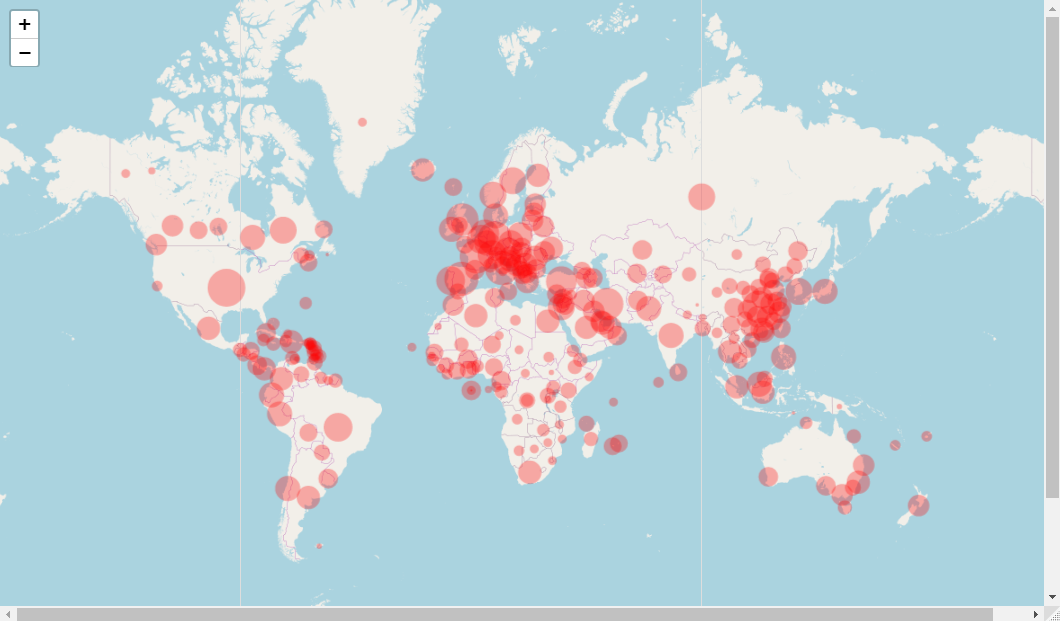
\includegraphics[width=1\linewidth,height=10cm]{anh/Rplot}  
	\vskip-4mm
	\caption{Bản đồ phân bố dịch COVID-19 trên toàn thế giới (7/4/2020)}
\end{figure}\\
Sau khi xử lí dữ liệu thô xong, chúng tôi có thể trích xuất dữ liệu đầy đủ theo ngày của bất kỳ quốc gia nào. Ở đây, chúng tôi lấy ví dụ là Việt Nam, bạn đọc có thể trích xuất dữ liệu của các quốc gia khác bằng cách thay "Vietnam" bằng tên của quốc gia đó.
\begin{lstlisting}
data %<>% filter(country=="Vietnam")
\end{lstlisting}
Tuy nhiên, chúng tôi không phân tích cụ thể từng quốc gia. Chúng tôi sẽ tiến hành phân tích tổng quan về tình hình dịch trên toàn thế giới. Đầu tiên, chúng tôi vẽ biểu đồ chuỗi thời gian về tổng số trường hợp ca nhiễm, số ca nhiễm hiện tại, số ca tử vong và số ca bình phục. Đồng thời, chúng tôi dùng hàm \textit{log} để tăng tỉ lệ giúp chúng ta dễ quan sát hơn. 
\begin{lstlisting}
world.long <- data.long %>% filter(country == "World")
## cases - area plot
plot1 <- world.long %>% filter(type != "Total Confirmed") %>%
ggplot(aes(x=date, y=count)) +
geom_area(aes(fill=type), alpha=0.5) +
labs(title=paste0("Numbers of Cases Worldwide - ", max.date.txt)) +
scale_fill_manual(values=c("red", "green", "black")) +
theme(legend.title=element_blank(), legend.position='bottom',
plot.title = element_text(size=8),
axis.title.x=element_blank(),
axis.title.y=element_blank(),
legend.key.size=unit(0.2, "cm"),
legend.text=element_text(size=6),
axis.text=element_text(size=7),
axis.text.x=element_text(angle=45, hjust=1))
plot2 <- world.long %>%
ggplot(aes(x=date, y=count)) +
geom_line(aes(color=type)) +
labs(title=paste0("Numbers of Cases Worldwide (log scale) - ", max.date.txt)) +
scale_color_manual(values=c("purple", "red", "green", "black")) +
theme(legend.title=element_blank(), legend.position='bottom',
plot.title = element_text(size=8),
axis.title.x=element_blank(),
axis.title.y=element_blank(),
legend.key.size=unit(0.2, "cm"),
legend.text=element_text(size=6),
axis.text=element_text(size=7),
axis.text.x=element_text(angle=45, hjust=1)) +
scale_y_continuous(trans="log10")
grid.arrange(plot1, plot2, ncol=2)
\end{lstlisting}
Chúng ta được kết quả chạy lệnh như hình \ref{h22}.
\begin{figure}[t]
	\centering
	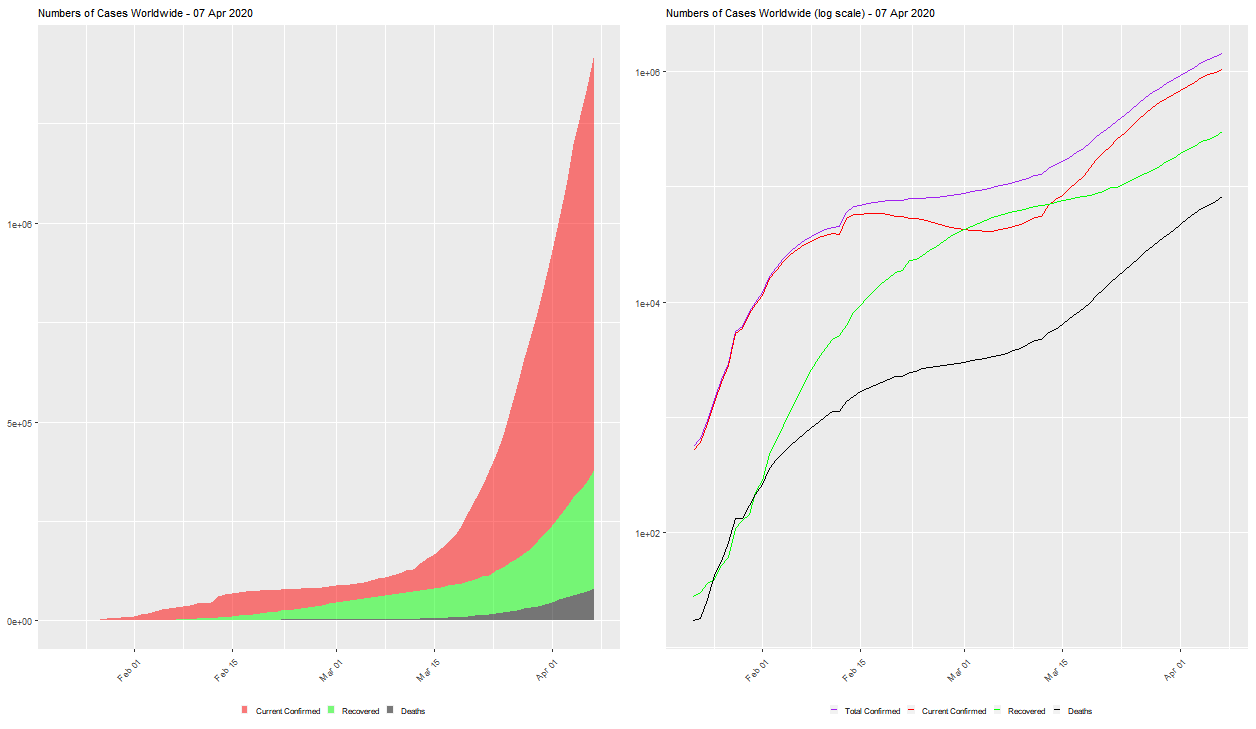
\includegraphics[width=1\linewidth,height=12cm]{anh/Rplot01}  
	\vskip-4mm
	\caption{Đồ thị dữ liệu chuỗi thời gian của COVID-19 trên toàn thế giới}
	\label{h22}
\end{figure}
Chúng tôi tiến hành xử lí số liệu bằng các lệnh trong R tương tự như xử lí số liệu thô ở phần \ref{xldlt} để hiển thị 20 quốc gia có số người nhiễm cao nhất hiện nay (7/4/2020).
\begin{lstlisting}
## ranking by confirmed cases
data.latest.all <- data %>% filter(date == max(date)) %>%
select(country, date,
confirmed, new.confirmed, current.confirmed,
recovered, deaths, new.deaths, death.rate=rate.lower) %>%
mutate(ranking = dense_rank(desc(confirmed)))
k <- 20
## top 20 countries: 21 incl. "World"
top.countries <- data.latest.all %>% filter(ranking <= k + 1) %>%
arrange(ranking) %>% pull(country) %>% as.character()
top.countries %>% setdiff("World")
## add "Others"
top.countries %<>% c("Others")
## put all others in a single group of "Others"
data.latest <- data.latest.all %>% filter(!is.na(country)) %>%
mutate(country=ifelse(ranking <= k + 1, as.character(country), "Others")) %>%
mutate(country=country %>% factor(levels=c(top.countries)))
data.latest %<>% group_by(country) %>%
summarise(confirmed=sum(confirmed), new.confirmed=sum(new.confirmed),
current.confirmed=sum(current.confirmed),
recovered=sum(recovered), deaths=sum(deaths), new.deaths=sum(new.deaths)) %>%
mutate(death.rate=(100 * deaths/confirmed) %>% round(1))
data.latest %<>% select(c(country, confirmed, deaths, death.rate,
new.confirmed, new.deaths, current.confirmed))
data.latest %>% mutate(death.rate=death.rate %>% format(nsmall=1) %>% paste0("%")) %>%
kable("latex", booktabs=T, row.names=T, align=c("l", rep("r", 6)),
caption=paste0("Cases in Top 20 Countries - ", max.date.txt),
format.args=list(big.mark=",")) %>%
kable_styling(font_size=7, latex_options=c("striped", "hold_position", "repeat_header"))
\end{lstlisting}
Kết quả của các dòng lệnh trên được mô tả trong bảng \ref{b25}.
\begin{table}[!h]	
	\caption{Top 20 quốc gia có số ca nhiễm cao nhất (7/4/2020)}\label{b25}
	\centering
	\fontsize{7}{9}\selectfont
	\begin{tabular}{llrrrrrr}
		\toprule
		& country & confirmed & deaths & death.rate & new.confirmed & new.deaths & current.confirmed\\
		\midrule
		\rowcolor{gray!6}  1 & World & 1,426,096 & 81,865 & 5.7\% & 80,995 & 7,300 & 1,044,177\\
		2 & US & 396,223 & 12,722 & 3.2\% & 29,556 & 1,939 & 361,738\\
		\rowcolor{gray!6}  3 & Spain & 141,942 & 14,045 & 9.9\% & 5,267 & 704 & 84,689\\
		4 & Italy & 135,586 & 17,127 & 12.6\% & 3,039 & 604 & 94,067\\
		\rowcolor{gray!6}  5 & France & 110,065 & 10,343 & 9.4\% & 11,102 & 1,417 & 80,199\\
		\addlinespace
		6 & Germany & 107,663 & 2,016 & 1.9\% & 4,289 & 206 & 69,566\\
		\rowcolor{gray!6}  7 & China & 82,718 & 3,335 & 4.0\% & 53 & 0 & 1,973\\
		8 & Iran & 62,589 & 3,872 & 6.2\% & 2,089 & 133 & 31,678\\
		\rowcolor{gray!6}  9 & United Kingdom & 55,949 & 6,171 & 11.0\% & 3,670 & 786 & 49,453\\
		10 & Turkey & 34,109 & 725 & 2.1\% & 3,892 & 76 & 31,802\\
		\addlinespace
		\rowcolor{gray!6}  11 & Switzerland & 22,253 & 821 & 3.7\% & 596 & 56 & 12,728\\
		12 & Belgium & 22,194 & 2,035 & 9.2\% & 1,380 & 403 & 16,002\\
		\rowcolor{gray!6}  13 & Netherlands & 19,709 & 2,108 & 10.7\% & 783 & 234 & 17,329\\
		14 & Canada & 17,872 & 375 & 2.1\% & 1,309 & 36 & 13,706\\
		\rowcolor{gray!6}  15 & Brazil & 14,034 & 686 & 4.9\% & 1,873 & 122 & 13,221\\
		\addlinespace
		16 & Austria & 12,639 & 243 & 1.9\% & 342 & 23 & 8,350\\
		\rowcolor{gray!6}  17 & Portugal & 12,442 & 345 & 2.8\% & 712 & 34 & 11,913\\
		18 & Korea, South & 10,331 & 192 & 1.9\% & 47 & 6 & 3,445\\
		\rowcolor{gray!6}  19 & Israel & 9,248 & 65 & 0.7\% & 344 & 8 & 8,413\\
		20 & Sweden & 7,693 & 591 & 7.7\% & 487 & 114 & 6,897\\
		\addlinespace
		\rowcolor{gray!6}  21 & Russia & 7,497 & 58 & 0.8\% & 1,154 & 11 & 6,945\\
		22 & Others & 143,340 & 3,990 & 2.8\% & 9,011 & 388 & 120,063\\
		\bottomrule
	\end{tabular}
\end{table}
Để trực quan hóa các dữ liệu từ bảng \ref{b25}, chúng tôi vẽ một biểu đồ có dữ liệu là số người nhiễm hiện tại và tỉ lệ tử vong của 20 quốc gia này.
\begin{lstlisting}
df <- data.latest %>% filter(country %in% setdiff(top.countries, "World"))
plot1 <- df %>% ggplot(aes(x=confirmed, y=deaths, col=death.rate, size=current.confirmed)) +
scale_size(name="Current Confirmed", trans="log2", breaks=c(1e3, 2e3, 5e3, 1e4, 2e4, 4e4)) +
geom_text(aes(label=country), size=2.5, check_overlap=T, vjust=-1.6) +
geom_point() +
xlab("Total Confirmed") + ylab("Total Deaths") +
labs(col="Death Rate (%)") +
scale_color_gradient(low="#56B1F7", high="#132B43") +
scale_x_log10() + scale_y_log10()
plot2 <- df %>% ggplot(aes(x=new.confirmed, y=new.deaths, col=death.rate, size=current.confirmed)) +
scale_size(name="Current Confirmed", trans="log2", breaks=c(1e3, 2e3, 5e3, 1e4, 2e4, 4e4)) +
geom_text(aes(label=country), size=2.5, check_overlap=T, vjust=-1.6) +
geom_point() +
xlab("New Confirmed") + ylab("New Deaths") +
labs(col="Death Rate (%)") +
scale_color_gradient(low="#56B1F7", high="#132B43") +
scale_x_log10() + scale_y_log10()
grid.arrange(plot1, plot2, ncol=1)
\end{lstlisting}
Chúng ta có được kết quả như hình \ref{h23}.
\begin{figure}[t]
	\centering
	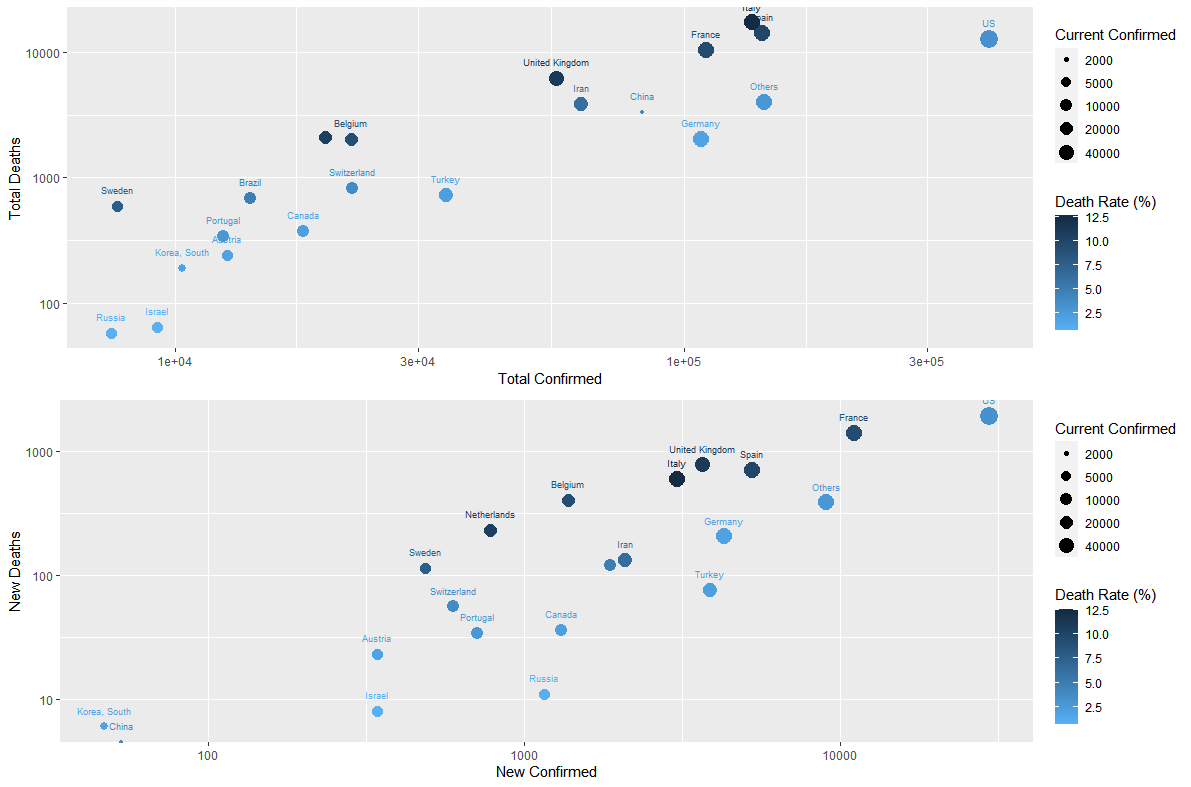
\includegraphics[width=1\linewidth,height=12cm]{anh/Rplot02}  
	\vskip-4mm
	\caption{Dồ thị thể hiện mức độ COVID-19 của top 20 quốc gia}
	\label{h23}
\end{figure}
Tiếp theo, chúng tôi thống kê Top 20 quốc gia có số tỉ lệ người tử vong cao nhất.
\begin{lstlisting}
## sort the latest data by death rate, and if tie, by confirmed
df <- data %>% filter(date == max(date) & country != "World" & confirmed >= 1000) %>%
select(country, confirmed, new.confirmed, current.confirmed,
recovered, deaths, new.deaths, death.rate=rate.lower) %>%
arrange(desc(death.rate, confirmed))
df %>% head(20) %>%
mutate(death.rate=death.rate %>% format(nsmall=1) %>% paste0("%")) %>%
kable("latex", booktabs=T, row.names=T, align=c("l", rep("r", 7)),
caption=paste0("Top 20 Countries with Highest Death Rates - ", max.date.txt),
format.args=list(big.mark=",")) %>%
kable_styling(font_size=7, latex_options=c("striped", "hold_position", "repeat_header"))
\end{lstlisting}
Kết quả của các lệnh trên được hiển thị ở bảng \ref{b26}.
\begin{table}[!h]
	\caption{Top 20 quốc gia có tỉ lệ tử vong cao nhất (7/4/2020)}
	\label{b26}
	\centering
	\fontsize{7}{9}\selectfont
	\begin{tabular}{llrrrrrrr}
		\toprule
		& country & confirmed & new.confirmed & current.confirmed & recovered & deaths & new.deaths & death.rate\\
		\midrule
		\rowcolor{gray!6}  1 & Algeria & 1,468 & 45 & 1,162 & 113 & 193 & 20 & 13.1\%\\
		2 & Italy & 135,586 & 3,039 & 94,067 & 24,392 & 17,127 & 604 & 12.6\%\\
		\rowcolor{gray!6}  3 & United Kingdom & 55,949 & 3,670 & 49,453 & 325 & 6,171 & 786 & 11.0\%\\
		4 & Netherlands & 19,709 & 783 & 17,329 & 272 & 2,108 & 234 & 10.7\%\\
		\rowcolor{gray!6}  5 & Spain & 141,942 & 5,267 & 84,689 & 43,208 & 14,045 & 704 & 9.9\%\\
		\addlinespace
		6 & France & 110,065 & 11,102 & 80,199 & 19,523 & 10,343 & 1,417 & 9.4\%\\
		\rowcolor{gray!6}  7 & Belgium & 22,194 & 1,380 & 16,002 & 4,157 & 2,035 & 403 & 9.2\%\\
		8 & Indonesia & 2,738 & 247 & 2,313 & 204 & 221 & 12 & 8.1\%\\
		\rowcolor{gray!6}  9 & Sweden & 7,693 & 487 & 6,897 & 205 & 591 & 114 & 7.7\%\\
		10 & Morocco & 1,184 & 64 & 1,001 & 93 & 90 & 10 & 7.6\%\\
		\addlinespace
		\rowcolor{gray!6}  11 & Egypt & 1,450 & 128 & 1,080 & 276 & 94 & 9 & 6.5\%\\
		12 & Iran & 62,589 & 2,089 & 31,678 & 27,039 & 3,872 & 133 & 6.2\%\\
		\rowcolor{gray!6}  13 & Iraq & 1,122 & 91 & 684 & 373 & 65 & 1 & 5.8\%\\
		14 & Ecuador & 3,747 & 0 & 3,456 & 100 & 191 & 0 & 5.1\%\\
		\rowcolor{gray!6}  15 & Mexico & 2,439 & 296 & 1,681 & 633 & 125 & 31 & 5.1\%\\
		\addlinespace
		16 & Dominican Republic & 1,956 & 128 & 1,822 & 36 & 98 & 12 & 5.0\%\\
		\rowcolor{gray!6}  17 & Brazil & 14,034 & 1,873 & 13,221 & 127 & 686 & 122 & 4.9\%\\
		18 & Philippines & 3,764 & 104 & 3,503 & 84 & 177 & 14 & 4.7\%\\
		\rowcolor{gray!6}  19 & Romania & 4,417 & 360 & 3,760 & 460 & 197 & 21 & 4.5\%\\
		20 & Greece & 1,832 & 77 & 1,482 & 269 & 81 & 2 & 4.4\%\\
		\bottomrule
	\end{tabular}
\end{table}
Quan sát các kết quả thống kê từ bảng \ref{b25} và \ref{b26}, chúng ta thấy được những con số rất khủng khiếp. Tuy nhiên, trung tâm Kiểm soát và Ngăn ngừa Dịch bệnh của châu Âu (ECDC) ngày 7/4 cho biết dịch bệnh viêm đường hô hấp cấp COVID-19 do virus SARS-CoV-2 gây ra đang lây lan và cướp đi sinh mạng của rất nhiều người tại khắp châu Âu, và hiện chưa có dấu hiệu nào cho thấy dịch COVID-19 tại châu lục này đã lên tới đỉnh.

Từ các kết quả phân tích tổng quan ở trên, chúng tôi sẽ tiến hành dự báo số ca nhiễm mới tại Mỹ và số ca tử vong mới tại Ý. Hai quốc gia này lần lượt có số người nhiễm và số ca tử vong cao nhất thế giới. Từ kết quả phân tích được, chúng tôi hy vọng kết quả này là hữu ích để chính phủ các nước có thể kiểm soát dịch bệnh tốt hơn.
\subsection{Dự báo số ca nhiễm mới và số ca tử vong do COVID-19 gây ra bằng mô hình ARIMA}
\subsubsection{Dự báo số ca nhiễm mới COVID-19 tại nước Mỹ}
Trong phần này, chúng tôi sẽ phân tích tình hình diễn biến dịch bệnh tại Mỹ và dự báo số ca nhiễm mới của quốc gia này trong 7 ngày tiếp theo.

Đã hơn hai tháng kể từ khi trường hợp nhiễm COVID-19 đầu tiên được chẩn đoán ở Mỹ. Kể từ đó, dịch đã lan rộng trên toàn quốc, với hơn 350000 ca nhiễm và gần 1300 ca tử vong (tính tại thời điểm ngày 7/4/2020). Hoa Kỳ trở thành tâm điểm toàn cầu của đại dịch khi vượt qua số ca nhiễm ở Trung Quốc - nơi mầm bệnh của COVID-19. Ông Anthony Fauci, giám đốc Viện Dị ứng và Bệnh Truyền nhiễm quốc gia đã phải thốt lên rằng COVID-19 thật sự là “một cơn ác mộng”. Ông nhận định rằng việc kiểm soát rất khó khăn vì có những thời điểm Mỹ tưởng như đã có thể kiểm soát được tình hình dịch bệnh khi cho rằng các ca nhiễm COVID-19 là co cụm (như ở trung tâm người già ở tiểu bang Washington), nhưng sau đó dịch bệnh lại bùng lên mạnh mẽ ở thành phố New York - nơi khách du lịch và người nhập cư đến rất nhiều. Nhận định sai lầm này khiến chính quyền Mỹ mất dấu, không còn khả năng kiểm soát mức độ lây lan của dịch bệnh.

Hoa Kỳ là một trong những quốc gia có nền y tế phát triển bậc nhất thế giới tuy nhiên vẫn tồn tại một số lỗ hổng nhất định. Và khi dịch bệnh bùng phát, sự phức tạp của nền y tế Mỹ dẫn đến một số vấn đề nghiêm trọng: (1) Một số người có dấu hiệu bệnh ban đầu nhưng không có bảo hiểm nên sợ đi khám, xét nghiệm khiến khả năng lây lan cộng đồng tăng cao; (2) Khi bắt đầu có triệu chứng, người bệnh buộc phải ra ngoài đến bệnh viện gặp bác sĩ khám, xin thuốc. Chính vì điều này khiến nguy cơ lây nhiễm tăng cao. Hơn nữa, COVID-19 xuất hiện vào thời điểm trọng yếu của chính trị Mỹ nên động thái xử lý dịch bệnh chậm trễ và thiếu dứt khoát ngay từ đầu.

Từ bức tranh tổng quan được nêu ra ở trên, chúng ta thấy rằng chỉ trong một thời gian ngắn, Mỹ từ một quốc gia không có dịch trở thành nước có số ca nhiễm dẫn đầu thế giới. Trước tình hình đó, việc dự báo diễn biến tình hình dịch bệnh ở Mỹ là việc hết sức quan trọng và cần thiết. Vì vậy, chúng tôi sẽ tiến hành dự báo số ca nhiễm mới trong 7 ngày tiếp theo.

Chúng tôi sử dụng dữ liệu được trích xuất từ ngày 22/1/2020 đến ngày 4/4/2020, sau đó chia chuỗi thời gian thành hai tập dữ liệu: tập "train" được dùng để đào tạo dữ liệu cho mô hình; tập "test" được dùng để kiểm tra và đánh giá hiệu suất của mô hình. Công việc này được thực thi trong R như sau:
\begin{lstlisting}
data %<>% filter(country=="US")
data.US <- data$new.confirmed[1:74] %>% ts()
train <- data$new.confirmed[1:70] %>% ts()
test <- data$new.confirmed[71:74] %>% ts()
\end{lstlisting}
\textbf{Bước 1: Kiểm tra tính dừng của tập "train".}\\
Vẽ biểu đồ chuỗi thời gian, đồ thị ACF và PACF.
\begin{lstlisting}
train %>% ggtsdisplay()
\end{lstlisting}
Ta được kết quả đầu ra như hình \ref{h24}. Quan sát biểu đồ chuỗi thời gian, ta thấy dữ liệu có xu hướng tăng trong thời gian dài nên chuỗi không có tính dừng. Hơn nữa, đồ thị ACF của chuỗi đã chỉ ra các spike (đỉnh) đang giảm từ từ - một dấu hiệu chuỗi thời gian không có tính dừng. Để chính xác hơn, chúng ta có thể kiểm tra tính dừng của một chuỗi dữ liệu bằng cách sử dụng thử nghiệm ADF.
\begin{lstlisting}
adf.test (train, alternative = "stationary")
##  	Augmented Dickey-Fuller Test
## data:  train
## Dickey-Fuller = 3.3984, Lag order = 4, p-value = 0.99
## alternative hypothesis: stationary
\end{lstlisting}
Ta thấy được $p-value = 0.99 > 0.05$, kết hợp với những ý nêu ra ở trên, chúng tôi kết luận chuỗi dữ liệu được quan sát không có tính dừng.\\
\begin{figure}[!htb]
	\centering
	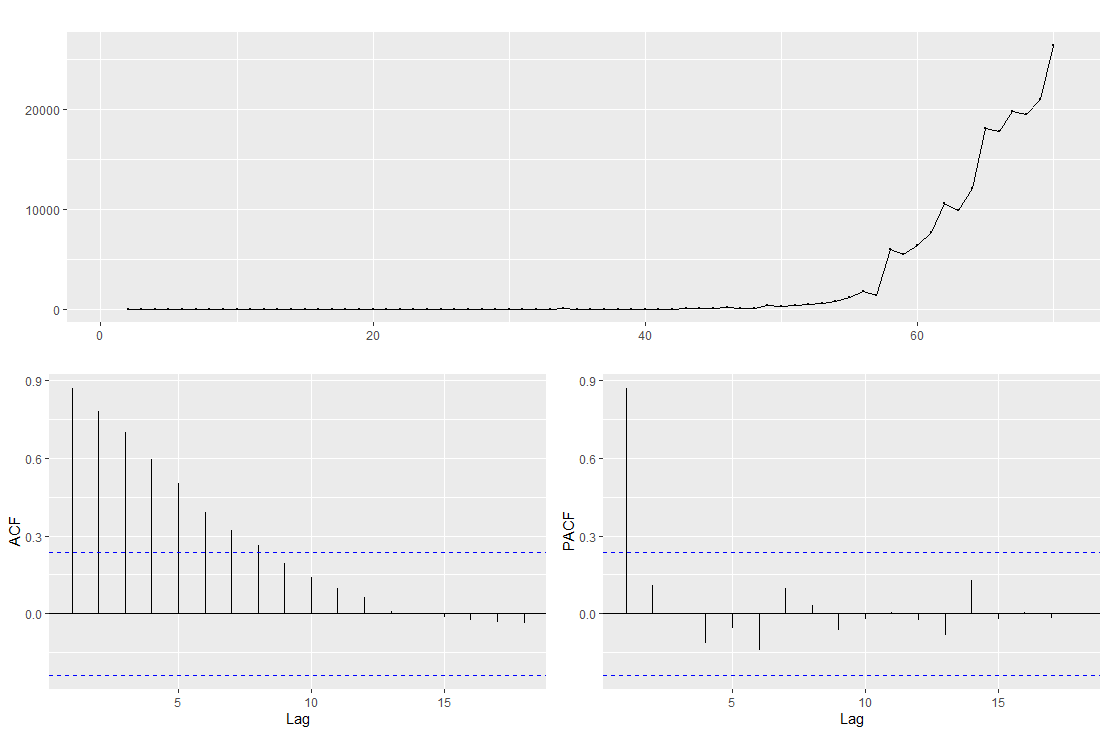
\includegraphics[width=1\linewidth,height=7.7cm]{anh/US1}
	\vskip-4mm 
	\caption{Đồ thị ACF và PACF của tập "train"}  
	\label{h24}
\end{figure}
\textbf{Bước 2: Chuyển chuỗi không dừng thành chuỗi dừng}\\
Thực hiện lấy sai phân bậc 1 và quan sát biểu đồ chuỗi thời gian, đồ thị ACF và PACF tương ứng. Thực hiện lệnh sau
\begin{lstlisting}
train %>% diff() -> diff1
diff1 %>% ggtsdisplay()
\end{lstlisting}
\begin{figure}[!htb]
	\centering
	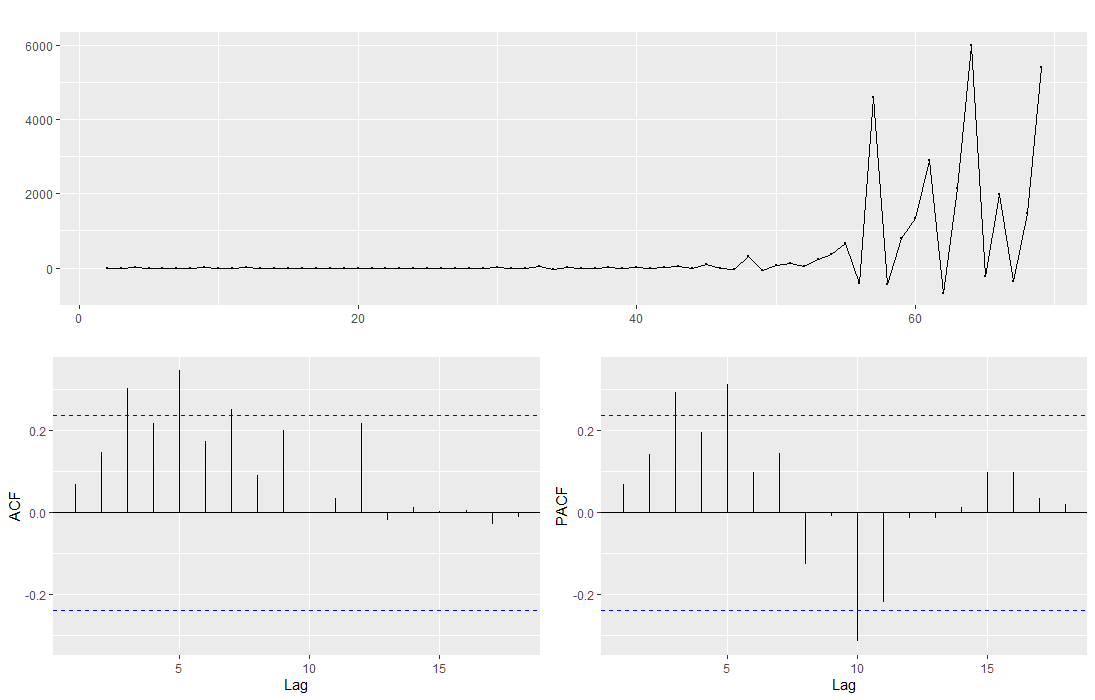
\includegraphics[width=1\linewidth,height=7.7cm]{anh/diff1}
	\vskip-4mm 
	\caption{Đồ thị ACF và PACF sau khi lấy sai phân bậc 1}  
	\label{diff1}
\end{figure}
Quan sát hình \ref{diff1}, chúng ta thấy chuỗi dữ liệu sau khi lấy sai phân bậc 1 chưa ổn định. Để chính xác hơn, chúng tôi tiến hành thử nghiệm ADF.\\
\begin{lstlisting}
adf.test (diff1, alternative = "stationary")
##  	Augmented Dickey-Fuller Test
## data:  train.diff
## Dickey-Fuller = -1.6228, Lag order = 4, p-value = 0.7283
## alternative hypothesis: stationary
\end{lstlisting}
Ta thấy $p-value = 0.7283 > 0.05$, chuỗi thời gian "diff1" chưa có tính dừng. Do đó, chúng tôi tiếp tục lấy sai phân bậc 2.
\begin{lstlisting}
train %>% diff() %>% diff() -> diff2
diff2 %>% ggtsdisplay()
\end{lstlisting}
\begin{figure}[!htb]
	\centering
	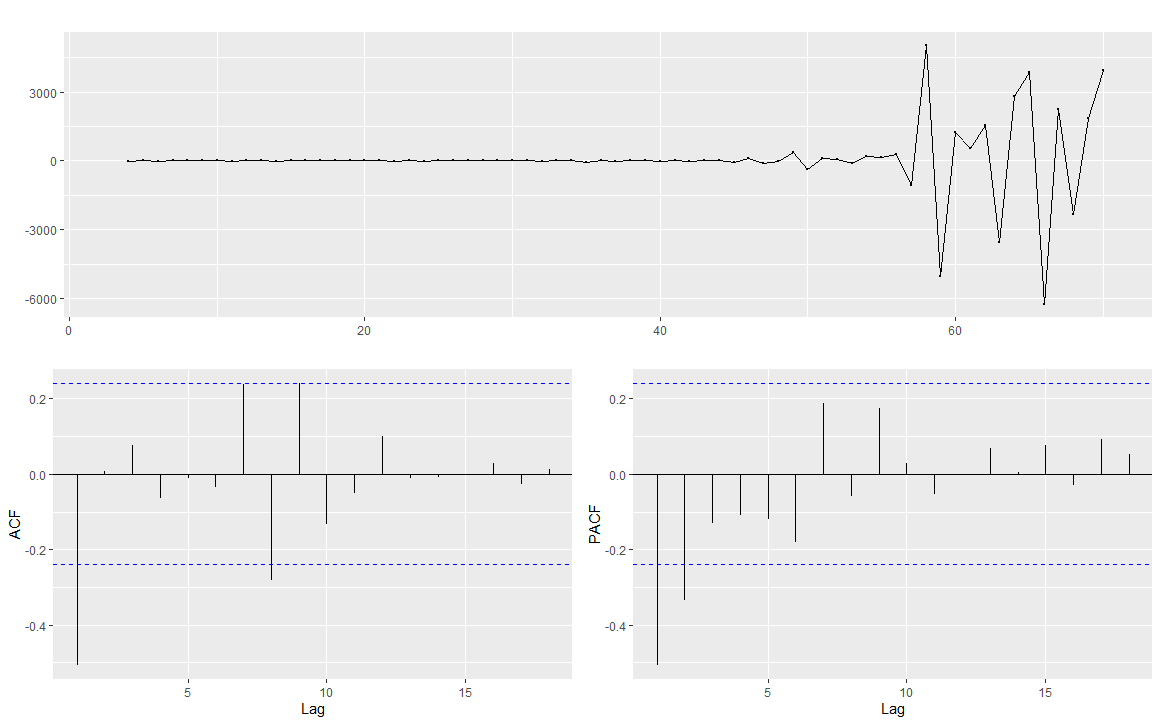
\includegraphics[width=1\linewidth,height=7.7cm]{anh/US2}
	\vskip-4mm 
	\caption{Đồ thị ACF và PACF sau khi lấy sai phân bậc 2}  
	\label{diff2}
\end{figure}
Quan sát hình \ref{diff2}, chúng ta thấy đồ thị "diff2" có giá trị trung bình và phương sai ổn định. Tiếp tục, ta dùng thử nghiệm ADF để kiểm tra.
\begin{lstlisting}
adf.test (train.diff, alternative = "stationary")	
## 	 Augmented Dickey-Fuller Test
## data:  train.diff
## Dickey-Fuller = -6.4328, Lag order = 4, p-value = 0.01
## alternative hypothesis: stationary
\end{lstlisting}
Kết quả của kiểm tra ADF cho thấy $p-value = 0.01 < 0.05$, kết hợp với các ý trên, ta kết luận chuỗi thời gian đã dừng sau khi lấy sai phân bậc 2.\\
Trong R, gói lệnh "forecast" giới thiệu cho chúng ta một hàm có thể gợi ý số lần lấy sai phân hợp lí cho một chuỗi thời gian bằng lệnh \lstinline{ndiffs(train)}. Thực hiện việc chạy lệnh, ta được kết quả là 2. Do vậy, để đưa chuỗi không dừng về chuỗi dừng, ta cần lấy sai phân bậc 2.\\
\textbf{Bước 3: Chọn mô hình thích hợp từ biểu đồ ACF và PACF}\\
Quan sát hình \ref{diff2}, dựa vào bảng \ref{b2}, chúng ta sẽ chọn được mô hình từ đồ thị ACF và PACF. Tại $lag$ 1 và $lag$ 8, các spike vượt ngoài đường giới hạn màu xanh gợi ý cho chúng ta thành phần MA(2). Các $lag$ 7 và $lag$ 9 nằm trên đường giới hạn nên không có ý nghĩa. Với việc lấy sai phân bậc 2 nên $d = 2$. Do đó, chúng ta có thể chọn được một mô hình đơn giản từ đồ thị ACF là ARIMA(0,2,2) $[AICc= 1116.71]$. Một cách tương tự, ta chọn được mô hình ARIMA(0,2,2) từ biểu đồ PACF. Do đó, chúng tôi chọn mô hình thích hợp từ ACF và PACF là ARIMA(0,2,2) $[AICc=1116.71]$.\\
\textbf{Bước 4: Khớp và chọn mô hình tốt nhất}\\
Tiếp theo, chúng ta tiến hành khớp (fit) mô hình bằng thuật toán Hyndman-Khandakar (2008) [Xem phụ lục \ref{H}] như trong bảng \ref{b27}.
\begin{table}[!h]
	\caption{Fit mô hình ARIMA cho dữ liệu số ca nhiễm mới COVID-19 tại Mỹ}\label{b27}
	\centering
	\fontsize{6}{10}\selectfont
	\begin{tabular}[t]{lrrrrr}
		\toprule
		STT	& ARIMA Models & AICc & RMSE train\\
		\midrule
		\rowcolor{gray!6}  1 & ARIMA(0,2,2) & 1116.71 & 904.6045\\
		2 & ARIMA(1,2,2) & 1116.61 & 887.8929\\
		\rowcolor{gray!6}  3 & ARIMA(0,2,3) & 1115.40  & 862.7566\\
		4 & ARIMA(1,2,3) & 1115.48 & 878.6758\\
		\rowcolor{gray!6} 5  & ARIMA(0,2,1) & 1135.40 & 1095.719\\
		\bottomrule
	\end{tabular}
\end{table}
Từ những mô hình được đưa ra trong bảng \ref{b27}, kết hợp với lý thuyết mô hình ARIMA và thước đo sai số RMSE, chúng tôi chọn mô hình ARIMA(0,2,3) là mô hình tốt nhất để báo (vì có các giá trị AICc và RMSE nhỏ nhất).\\ 
\textbf{Bước 5: Kiểm tra phần dư từ mô hình được chọn}\\
Trước khi dự báo, chúng ta kiểm tra phần dư từ mô hình đã chọn bằng cách vẽ ACF của phần dư. Nếu biểu đồ phần dư không giống nhiễu trắng, hãy thử một mô hình khác bằng cách quay lại bước 3 và thực hiện các bước tiếp theo. Chúng ta thực hiện lệnh kiểm tra phần dư như sau
\begin{lstlisting}
best.md <- Arima(train, order = c(0,2,3))
checkresiduals(best.md)
##  	Ljung-Box test
## data:  Residuals from ARIMA(0,2,3)
## Q* = 7.7973, df = 7, p-value = 0.3508
## Model df: 3.   Total lags used: 10
\end{lstlisting}
\begin{figure}[!htb]
	\centering
	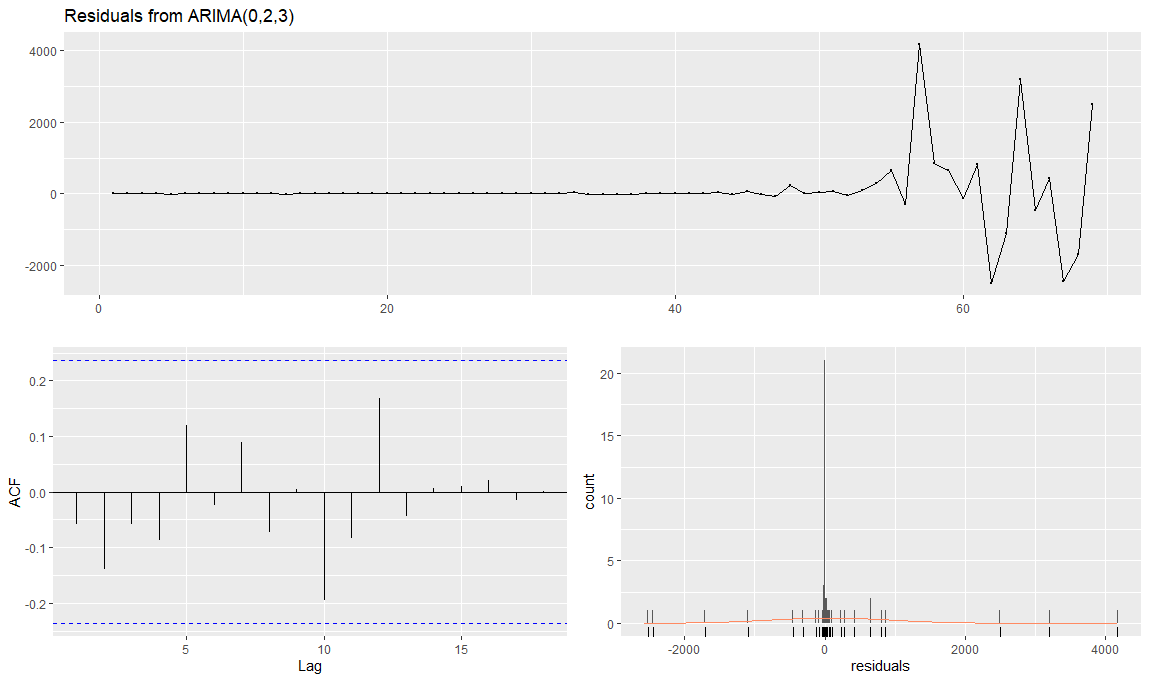
\includegraphics[width=1\linewidth,height=7.7cm]{anh/NT1}
	\vskip-4mm 
	\caption{Đồ thị ACF phần dư của mô hình ARIMA(0,2,3)}  
	\label{NT1}
\end{figure}
Quan sát hình \ref{NT1}, các spike đều nằm trong khoảng giới hạn và đồ thị ACF phần dư không có spike đột biến. Vì vậy mô hình của chúng ta đã vượt qua các bài kiểm tra và sẵn sàng để tính toán dự báo.\\
\textbf{Bước 6: Đánh giá sai số của mô hình trên tập "train" và dự báo}\\
Tiếp theo, chúng ta tiến hành kiểm tra sai số từ mô hình ARIMA(0,2,3) bằng cách dự báo cho 4 ngày tiếp theo và so sánh với 4 ngày thực tế trên tập "test". Các câu lệnh được thực hiện như sau
\begin{lstlisting}
best.md <- Arima(train, order = c(0,2,3))
test.fc <- forecast(best.md, h = 4)$mean %>% as.vector()
df_md <-  tibble(Actual = test %>% as.vector(), 
Forecast = test.fc %>% round(0), 
Error = Forecast - Actual,
Error_Percent = round(Error / Actual, 2))
df_md %>% kable("latex", booktabs=T, caption="Error from ARIMA(0,2,3) model") %>%
kable_styling(font_size=6, latex_options = c("striped", "hold_position", "repeat_header"))
\end{lstlisting}
\begin{table}[!h]	
	\caption{Đánh giá sai số từ mô hình ARIMA(0,2,3)}
	\label{u1}
	\centering
	\fontsize{6}{8}\selectfont
	\begin{tabular}[t]{rrrrr}
		\toprule
		Date &Actual & Forecast & Error & Error\_Percent\\
		\midrule
		\rowcolor{gray!6} 2020-04-01 &25200 & 26711 & 1511 & 6\%\\
		2020-04-02 &30390 & 27733 & -2657 & -9\%\\
		\rowcolor{gray!6} 2020-04-03 &31824 & 29476 & -2348 & -7\%\\
	    2020-04-04 &33267 & 31219 & -2048 & -6\%\\
		\bottomrule
	\end{tabular}
\end{table}
Từ bảng \ref{u1} chúng tôi rút ra một số nhận xét như sau:
\begin{itemize}
	\item[(i)] Phần trăm sai số giữa các giá trị dự báo và giá trị thực tế tương đối nhỏ.
	\item[(ii)] Giá trị dự báo thấp hơn so với giá trị thực tế. Điều này cho chúng ta thấy rằng số ca nhiễm mới tại Mỹ đang tăng rất nhanh và có nguy cơ sẽ dẫn đến khủng hoảng trên diện rộng trong vài ngày tới. Vì vậy các giá trị dự báo được đánh giá là phù hợp và có ý nghĩa.
\end{itemize}
Do đó, mô hình này có thể là mô hình có ích để đưa ra một cảnh báo cấp thiết và có hành động cao hơn nữa nhằm kiểm soát tốt dịch bệnh trong thời gian tới. Chúng tôi chọn mô hình ARIMA(0,2,3) để dự báo số ca nhiễm mới COVID-19 trên toàn thế giới trong 7 ngày tiếp theo.
\begin{lstlisting}
final_md <- Arima(data.US, order = c(0,2,3))
new.Confirmed <- forecast(final_md, h = 7)
new.Confirmed %>% kable("latex", booktabs=T, caption="New Confirmed in USA - Forecast") %>% kable_styling(font_size=6, latex_options = c("striped", "hold_position", "repeat_header"))
plot_forecast(new.Confirmed, title = "New Confirmed in USA - Forecast",
Ytitle = "Case Number",
Xtitle = "Date")
\end{lstlisting}
\begin{table}[!h]	
	\caption{Dự báo số ca nhiễm mới COVID-19 tại Mỹ trong 7 ngày tiếp theo}
    \label{b30}
	\centering
	\fontsize{6}{8}\selectfont
	\begin{tabular}[t]{lrrrrr}
		\toprule
		& Point Forecast & Lo 80 & Hi 80 & Lo 95 & Hi 95\\
		\midrule
		\rowcolor{gray!6}  75 & 35795.23 & 34513.19 & 37077.28 & 33834.52 & 37755.95\\
		76 & 38739.10 & 37311.61 & 40166.59 & 36555.94 & 40922.26\\
		\rowcolor{gray!6}  77 & 41727.88 & 40074.77 & 43380.99 & 39199.66 & 44256.10\\
		78 & 44716.66 & 42636.16 & 46797.16 & 41534.81 & 47898.51\\
		\rowcolor{gray!6}  79 & 47705.44 & 45023.33 & 50387.55 & 43603.51 & 51807.37\\
		\addlinespace
		80 & 50694.22 & 47274.09 & 54114.35 & 45463.59 & 55924.85\\
		\rowcolor{gray!6}  81 & 53683.00 & 49415.92 & 57950.08 & 47157.06 & 60208.94\\
		\bottomrule
	\end{tabular}
\end{table}
\begin{figure}[!htb]
	\centering
	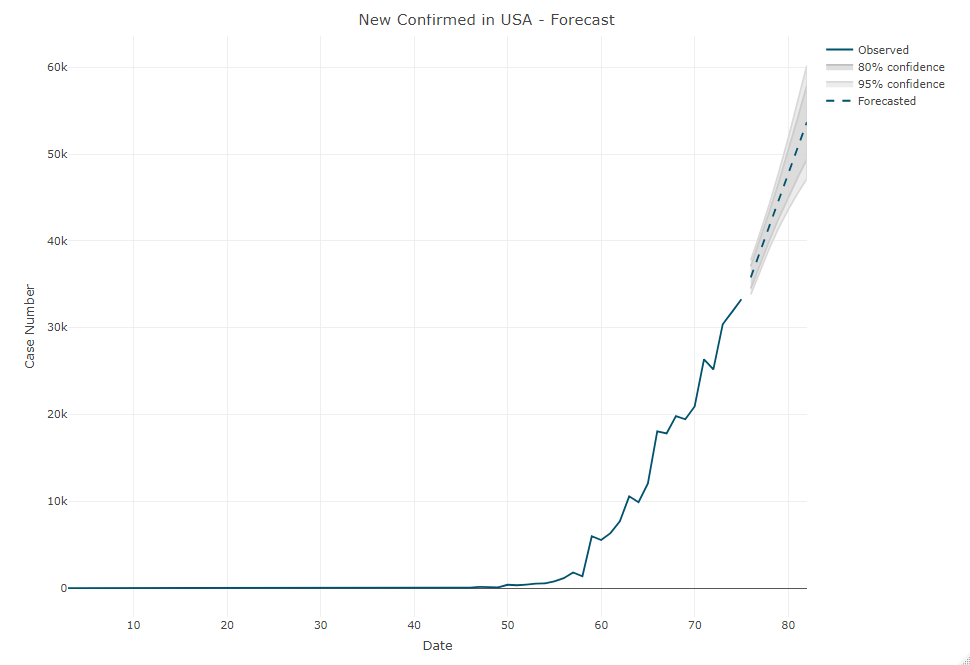
\includegraphics[width=1\linewidth, height=7.7cm]{anh/A7}
	\vskip-4mm 
	\caption{Đồ thị dự báo số ca nhiễm mới COVID-19 tại Mỹ trong 7 ngày tiếp theo}  
	\label{hu1}
\end{figure}
Dựa vào bảng \ref{b30} và hình \ref{hu1}, chúng tôi thấy đồ thị có xu hướng đi lên và không có dấu hiệu giảm. Do đó, chúng tôi sẽ đưa ra một cảnh báo cho 7 ngày tiếp theo (5/4/2020 - 11/4/2020) rằng số ca nhiễm tại nước Mỹ vẫn tiếp tục tăng cao, thậm chí vượt khỏi giới hạn trên của khoảng dự báo 95\% nếu Mỹ không có các biện pháp mạnh hơn nữa.\\
\textbf{Các nước rút ra được bài học gì từ Mỹ?}\\
\begin{itemize}
    \item Bài học lớn nhất từ Dr. Fauci: Nếu ở những nơi ca nhiễm còn thấp (dưới 200 ca) thì việc cách ly, lần dấu vết xem ai lây cho ai, xét nghiệm diện rộng là rất quan trọng. Tuy nhiên, với quy mô xét nghiệm còn hạn chế như ở Mỹ và chưa được thực hiện triệt để như Việt nam. Còn những nơi ca nhiễm đã rất cao và lây lan cộng đồng rồi (tức là đã mất kiểm soát) thì không còn cách nào khác là đóng cửa mọi nơi, mọi người tự cách ly tại nhà để giảm áp lực lên hệ thống y tế.
   \item Chiến lược xét nghiệm cộng đồng là rất cần thiết ngay lúc này. Chúng tôi sẽ ra 2 lý do cho việc làm này như sau
\begin{itemize}
	\item \textit{Có bao nhiêu ca nhiễm không có triệu chứng?} Để trả lời câu hỏi có bao nhiêu ca nhiễm mà không biểu hiện triệu chứng, một nhóm nghiên cứu đã phân tích số liệu thu thập từ du thuyền Diamond Princess. Cần nhớ rằng du thuyền Diamond Princess có 3711 hành khách và thủy thủ đoàn, và trong số này có 619 người (17\%) bị nhiễm. Một phân tích sâu hơn cho thấy trong số những ca bị nhiễm, có đến 18\% không hề biểu hiện triệu chứng \cite{13}. Do vậy, các ca nhiễm không biểu hiện triệu chứng nhưng vẫn có thể lây nhiễm. 
	\item \textit{Những ca nhiễm không phát hiện được}. Một phân tích khác từ Vũ Hán cho ra kết quả rất ngạc nhiên! Theo họ ước tính, có khoảng 59\% những ca bị nhiễm "lang thang" trong cộng đồng. Những người này không hề được xét nghiệm, có lẽ không có triệu chứng, nhưng họ có thể lây nhiễm sang người khác. Điều này có thể giải thích tại sao mức độ lây lan của virus rất nhanh (theo cấp số nhân) khi được phát hiện \cite{14}. Ngoài ra, tập san Science mới công bố một phân tích rất phức tạp cho thấy số ca nhiễm không được phát hiện lên đến 86\% \cite{15}!
\end{itemize}
\end{itemize}
\subsubsection{Dự báo số ca tử vong mới theo ngày do COVID-19 gây ra ở Italy}
Trong phần này, chúng tôi đưa ra nguyên nhân dẫn đến số ca tử vong tăng vọt tại Ý và dự báo số ca tử vong mới tại quốc gia này trong 7 ngày tiếp theo bằng mô hình ARIMA.

Tại Italy, Cơ quan Bảo vệ Dân sự xác nhận thêm 3.039 ca dương tính với SARS-CoV-2 trong ngày 7/4. Mặc dù đây là số ca nhiễm mới thấp nhất kể từ ngày 17/3 tại quốc gia này, nhưng số ca tử vong lại tăng lên rất cao. Có thêm 604 ca tử vong do SARS-CoV-2 ở Italy, nâng tổng số bệnh nhân COVID-19 thiệt mạng lên đến 17.127 người - mức cao nhất trên thế giới. Vậy nguyên nhân dẫn đến sự tăng vọt này là gì? Nhóm Ioannidis vừa có một bài báo được đăng trên tạp chí JAMA Int Med đưa ra những quan điểm trả lời cho câu hỏi trên \cite{16}. Theo đó, số ca tử vong ở Ý có sự biến chuyển là vì:
\begin{itemize}
	\item Yếu tố lão hóa dân số: Ý có dân số già bậc nhất châu Âu. Gần một phần tư (23\%) dân số của nước này có độ tuổi từ 65 trở lên. Hơn thế, những người này tiền sử bệnh như hô hấp, tim mạch, tiểu đường và ung thư. Do đó, gánh nặng dịch bệnh đã đè lên bệnh trạng sẵn có.
	\item Hệ thống y tế: mặc dù Ý là nước có hệ thống y tế Nhà nước rất tốt, nhưng số giường bệnh ICU thì rất khiêm tốn (toàn quốc chỉ có 5090 giường, tức 8.4 trên 100,000 dân).
\end{itemize}

Trước tình hình đó, chính phủ Ý rất khó để kiểm soát dịch bệnh và cũng vì thế số ca tử vong liên tục tăng cao. Chúng tôi sẽ tiến hành dự báo số ca tử vong mới do COVID-19 ở Ý trong 7 ngày tiếp theo dựa trên dữ liệu số ca tử vong hàng ngày ở Ý được trích xuất trong "data" từ ngày 22-01-2020 đến ngày 07/04/2020. Tương tự như trên, chúng tôi tiến hành chia tập dữ liệu thành tập "train" và "test" để đào tạo, kiểm tra và đánh giá hiệu suất mô hình.\\
\begin{lstlisting}
data %<>% filter(country=="Italy")
data.Italy <- data$new.deaths[1:77] %>% ts()
train <- data$new.deaths[1:72] %>% ts()
test <- data$new.deaths[73:77] %>% ts()
\end{lstlisting}
Trong R, để xây dựng mô hình ARIMA tốt nhất cho dự báo, chúng tôi sử dụng hàm \lstinline{auto.arima} [dựa trên thuật toán Hyndman-Khandakar (2008)].
\textbf{Bước 1: Vẽ và quan sát đồ thị dữ liệu số ca tử vong mới tại Ý}\\
\begin{lstlisting}
autoplot(train) + ggtitle("Data new deaths in Italy") + 
theme(plot.title = element_text(hjust = 0.5)) + 
xlab("Date") +
ylab("Case number")
\end{lstlisting}
\begin{figure}[!htb]
	\centering
	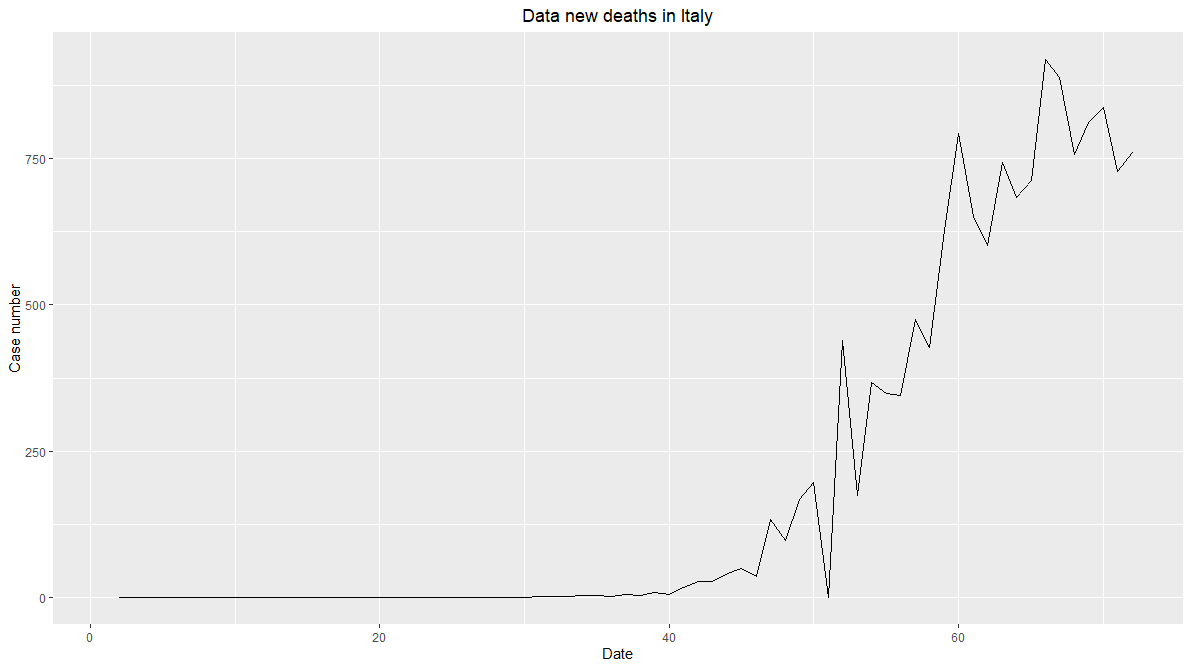
\includegraphics[width=1\linewidth, height=7.7cm]{anh/I1}
	\vskip-4mm 
	\caption{Đồ thị số ca tử vong mới do COVID-19 tại Ý}  
	\label{I1}
\end{figure}
Quan sát hình \ref{I1}, chúng ta thấy chuỗi dữ liệu không có tính dừng. Thay vì lấy sai phân, chúng tôi sẽ giới thiệu một thuật toán tự động tìm ra mô hình tốt nhất.\\
\textbf{Bước 2: Sử dụng hàm "auto.arima" để tìm ra mô hình tốt nhất}\\
Chúng tôi sử dụng hàm \lstinline{auto.arima} để đưa ra mô hình tốt nhất dựa theo thuật toán Hyndman-Khandakar (2008) [Xem phụ lục \ref{H}].
\begin{lstlisting}
arima.Italy <- auto.arima(train)

## Best model: ARIMA(3,1,3) 
## Coefficients:
##          ar1     ar2    ar3      ma1      ma2     ma3
##       0.0056  0.7302  0.057  -0.9051  -0.6095  0.8668
## s.e.  0.2056  0.1923  0.132   0.2259   0.3003  0.2290
## sigma^2 estimated as 4356:  log likelihood=-392.39
## AIC=798.77   AICc=800.58   BIC=814.51
\end{lstlisting}
Từ kết quả chạy lệnh, chúng tôi chọn mô hình ARIMA(3,1,3) là mô hình tốt nhất để dự báo.\\
\textbf{Bước 3: Kiểm tra phần dư từ mô hình ARIMA(3,1,3)}\\
Sau khi tìm được mô hình tốt nhất, chúng tôi tiến hành kiểm tra phần dư từ mô hình. Nếu phần dư không phải nhiễu trắng thì thực hiện việc lấy sai phân và chọn mô hình từ đồ thị ACF và PACF. Chúng tôi thực hiện lệnh kiểm tra phần dư như sau\\ 
\begin{lstlisting}
checkresiduals(arima.Italy)

##  	Ljung-Box test
## data:  Residuals from ARIMA(3,1,3)
## Q* = 9.4822, df = 4, p-value = 0.05011
## Model df: 6.   Total lags used: 10
\end{lstlisting}
\begin{figure}[!htb]
	\centering
	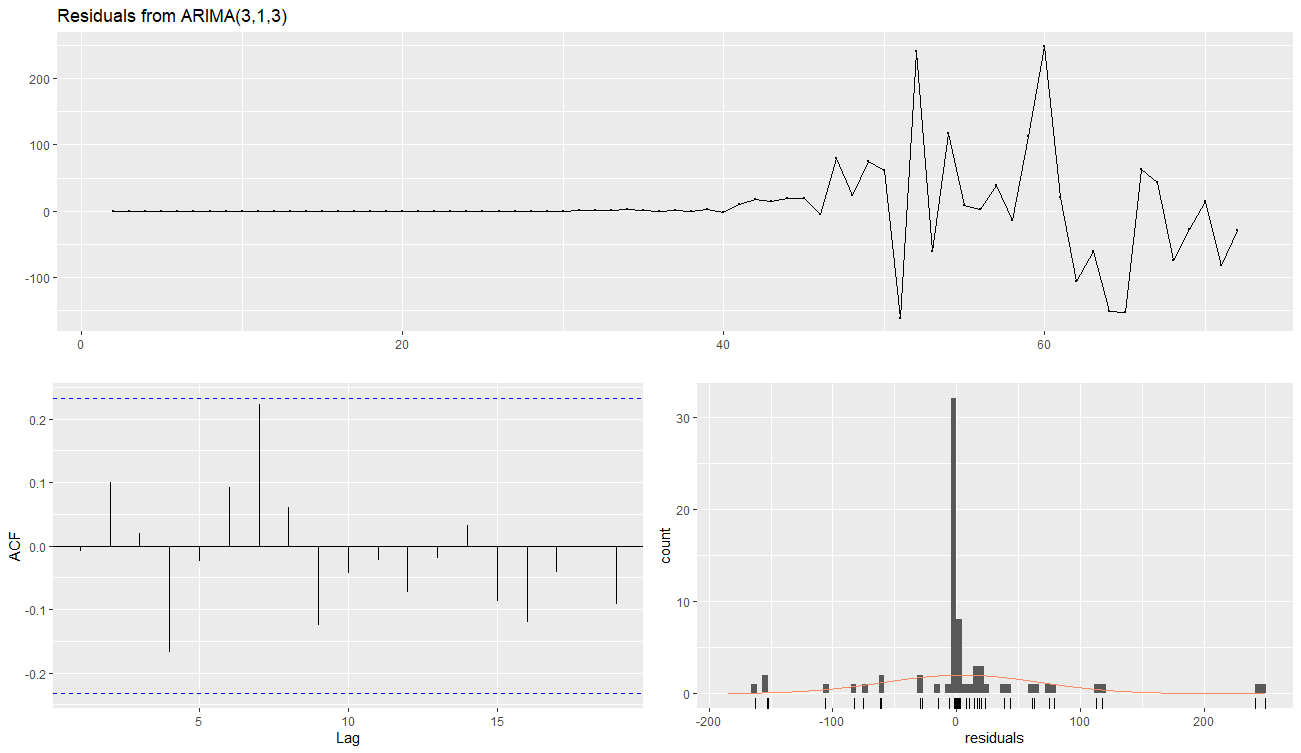
\includegraphics[width=1\linewidth, height=7.7cm]{anh/PD1}
	\vskip-4mm 
	\caption{Đồ thị kiểm tra phần dư từ mô hình ARIMA(3,1,3)}  
	\label{PD1}
\end{figure}
Quan sát hình \ref{PD1}, chúng ta thấy ACF phần dư có các spike đều nằm trong khoảng giới hạn và không có spike đột biến. Do đó, mô hình ARIMA(3,1,3) là hợp lý và được chọn để tính toán dự báo.\\
\textbf{Bước 4: Đánh giá sai số từ mô hình ARIMA(3,1,3) và dự báo}\\
Chúng tôi thực hiện dự báo cho 5 ngày tiếp theo của tập "train" và đánh giá sai số dựa vào giá trị thực của tập "test".
\begin{lstlisting}
# Use the model for forecasting: 
forecast_arima <- forecast(arima.Italy, h = 5)$mean %>% as.vector()
df_arima <-  tibble(Actual = test %>% as.vector(), 
Forecast = forecast_arima %>% round(0), 
Error = Forecast - Actual,
Error_Percent = round(Error / Actual, 2))
\end{lstlisting}
\begin{table}[!h]	
	\caption{Đánh giá sai số dự báo số ca tử vong mới ở Ý}
    \label{Italy}
	\centering
	\fontsize{6}{8}\selectfont
	\begin{tabular}[t]{rrrrr}
		\toprule
		Date & Actual & Forecast & Error & Error\_Percent\\
		\midrule
		\rowcolor{gray!6}  2020-04-03 & 766 & 770 & 4 & 1\%\\
		2020-04-04 & 681 & 735 & 54 & 8\%\\
		\rowcolor{gray!6}  2020-04-05 & 525 & 720 & 195 & 37\%\\
		2020-04-06 & 636 & 694 & 58 & 9\%\\
		\rowcolor{gray!6}  2020-04-07 & 604 & 681 & 77 & 13\%\\
		\bottomrule
	\end{tabular}
\end{table}
Quan sát bảng \ref{Italy}, chúng ta thấy được phần trăm sai số và độ lệnh là rất nhỏ. Vì vậy mô hình này có thể dùng để dự báo tổng quan cho 7 ngày tiếp theo tại Ý.
\begin{lstlisting}
model.new.deaths <- Arima(data.Italy, order = c(3,1,3))
forecast.new.deaths <- forecast(model.new.deaths, h = 7)
\end{lstlisting}
\begin{table}[!h]
	\caption{Dự báo số ca tử vong mới tại Ý trong 7 ngày tiếp theo}
	\label{tab:}
	\centering
	\fontsize{6}{8}\selectfont
	\begin{tabular}[t]{lrrrrr}
		\toprule
		& Point Forecast & Lo 80 & Hi 80 & Lo 95 & Hi 95\\
		\midrule
		\rowcolor{gray!6}  78 & 521.8161 & 435.4723 & 608.1600 & 389.76460 & 653.8677\\
		79 & 487.9330 & 400.8170 & 575.0490 & 354.70053 & 621.1654\\
		\rowcolor{gray!6}  80 & 433.8354 & 344.6312 & 523.0397 & 297.40930 & 570.2616\\
		81 & 400.5004 & 302.0105 & 498.9904 & 249.87302 & 551.1279\\
		\rowcolor{gray!6}  82 & 356.1975 & 247.7964 & 464.5986 & 190.41228 & 521.9827\\
		\addlinespace
		83 & 325.4238 & 200.2443 & 450.6032 & 133.97834 & 516.8692\\
		\rowcolor{gray!6}  84 & 288.5974 & 146.3005 & 430.8943 & 70.97312 & 506.2218\\
		\bottomrule
	\end{tabular}
\end{table}
\begin{lstlisting}
plot_forecast(forecast.new.deaths, title = "New Deaths in Italy - Forecast",
Ytitle = "Case Number",
Xtitle = "Date")
\end{lstlisting}
\begin{figure}[!htb]
	\centering
	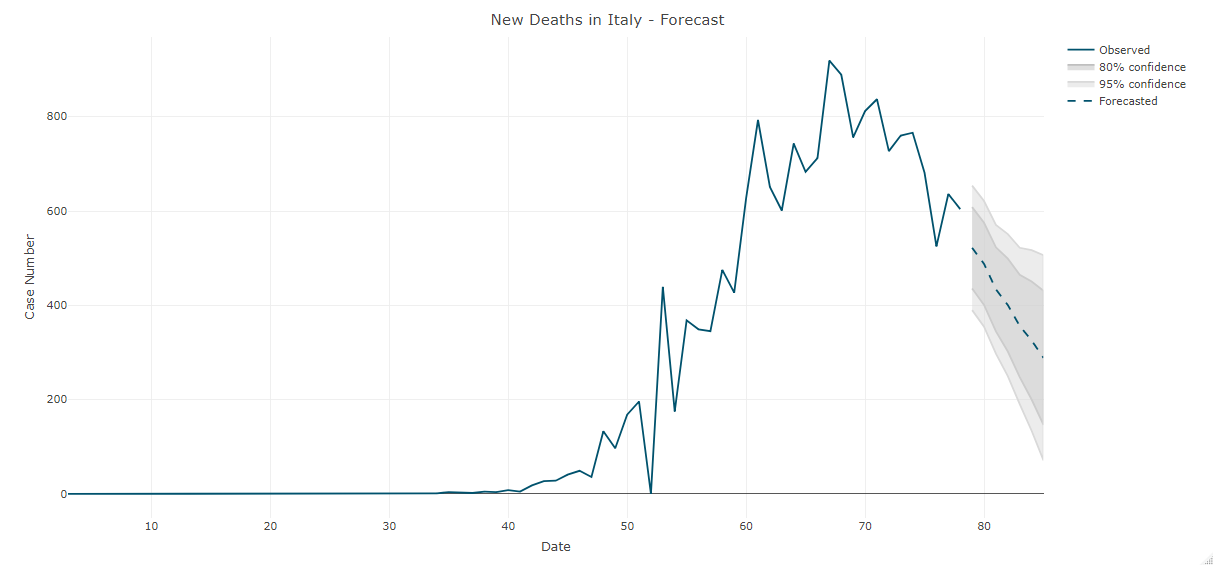
\includegraphics[width=1\linewidth,height=7.7cm]{anh/A8}
	\vskip-4mm 
	\caption{Đồ thị dự báo số ca nhiễm mới COVID-19 tại Ý trong 7 ngày tiếp theo}  
	\label{A8}
\end{figure}
Từ hình \ref{A8}, chúng ta thấy số ca tử vong mới ở Ý có xu hướng giảm trong tuần tới. Tuy nhiên con số tử vong vẫn còn rất cao. Do đó, chính phủ Ý không nên chủ quan mà cần nỗ lực hơn nữa để đưa ra kịch bản kiểm soát dịch và phác đồ điều trị tối ưu nhất.

\section{Dự báo lượng mưa hàng tháng tại trạm quan trắc Quy Nhơn}
Trong phần này, chúng tôi sẽ phân tích tổng quan lượng mưa tại trạm quan trắc Quy Nhơn và dự báo lượng mưa trung bình hàng tháng cho 2 năm tiếp theo bằng mô hình mô hình tự hồi quy tích hợp trung bình trượt theo mùa (SARIMA).

Lượng mưa là một trong những hiện tượng quan trọng nhất của hệ thống tự nhiên có ảnh hưởng chung đến biến đổi khí hậu. Do đó, việc mô hình hóa và dự báo nó là cần thiết để giải quyết một số vấn đề liên quan đến quy hoạch và quản lí hệ thống tài nguyên nước, công trình thủy lợi, quản lí nông nghiệp, ... . Tuy nhiên, dự báo lượng mưa là khó khăn vì nó có dạng là mô hình phi tuyến tính và thay đổi lớn về cường độ. Cho đến hôm nay, có rất nhiều kỹ thuật đã được sử dụng để dự báo lượng mưa. Trong đó, mô hình ARIMA theo mùa (SARIMA) có nhiều ưu điểm hơn so với các mô hình khác, đặc biệt là so với các mô hình làm mịn theo hàm mũ và mạng noron \cite{17}. Mô hình ARIMA xem xét mối tương quan nối tiếp đó là đặc trưng quan trọng nhất của dữ liệu chuỗi thời gian. Một ưu điểm của mô hình ARIMA là việc sử dụng mô hình ít tham số để mô tả một chuỗi thời gian.

Mô hình ARIMA theo mùa được sử dụng rộng rãi để dự báo khí tượng thủy văn. Rahman và các cộng sự đã có một bài nghiên cứu đánh giá giữa 2 mô hình ARIMA và ANFIS để dự báo thời tiết cho thành phố Dhaka, kết quả cho thấy mô hình ARIMA thực hiện tốt hơn ANFIS \cite{18}. Dizon công bố kết quả nghiên cứu về ARIMA theo mùa là một mô hình rất tốt cho dự báo chuỗi thời gian có tính mùa vụ mạnh \cite{19}. Momani sử dụng thành công mô hình ARIMA để dự báo xu hướng lượng mưa của Jordan \cite{20}. Tại Việt Nam, Nguyễn Hữu Quyền đã có một bài luận văn thạc sĩ khoa học về ứng dụng mô hình động thái ARIMAX để dự báo lượng mưa vụ đông xuân ở một số tỉnh vùng đồng bằng Bắc Bộ \cite{21}. Chính vì vậy, mô hình ARIMA theo mùa có thể được xem là một công cụ hữu ích để dự báo hiện tượng khí tượng thủy văn, đặc biệt là lượng mưa.

Chúng tôi lấy dữ liệu của trạm quan trắc Quy Nhơn từ \textit{Trung tâm dữ liệu khí tượng thủy văn quốc gia} (\url{http://cmh.com.vn/}). Dữ liệu được thống kê từ tháng 1/2000 đến tháng 12/2018,  bạn đọc có thể quan sát số liệu tại bảng \ref{datarainfall}. Tương tự như các ví dụ ở trên, chúng tôi trích xuất dữ liệu của 18 năm đầu (tương ứng với 216 tháng) thành tập "train" và 12 tháng của năm 2018 là tập "test". Dữ liệu lượng mưa hàng tháng là chuỗi thời gian có tính chất mùa vụ. Vì vậy chúng tôi sẽ sử dụng mô hình SARIMA (hay ARIMA theo mùa) với tần số là 12 để dự báo cho 2 năm tiếp theo. Dữ liệu sẽ được phân tích trực tiếp trong R với các gói package được sử dụng như trong phần (\ref{xldlt}).
\subsection{Tổng quan về đặc điểm lượng mưa tại trạm quan trắc Quy Nhơn}
Đối với các dữ liệu có tính mùa vụ, chúng tôi giới thiệu hàm vẽ đồ thị chuỗi thời gian theo mùa vụ được phát triển bởi Hyndman và Athanasopoulos để mô tả đặc điểm mùa vụ tại trạm quan trắc Quy Nhơn.
\begin{lstlisting}
mydata <- read.xlsx("mydata.xlsx")
rainfall <- ts(mydata, start = c(2000,1), frequency = 12)
ggseasonplot(rainfall, year.labels=TRUE, year.labels.left=TRUE) +
theme(plot.title = element_text(hjust = 0.5)) +  
ylab("Total monthly rainfall (mm)") +
ggtitle("Seasonal plot: Total monthly rainfall in Quy Nhon")
\end{lstlisting}
\begin{figure}[!htb]
	\centering
	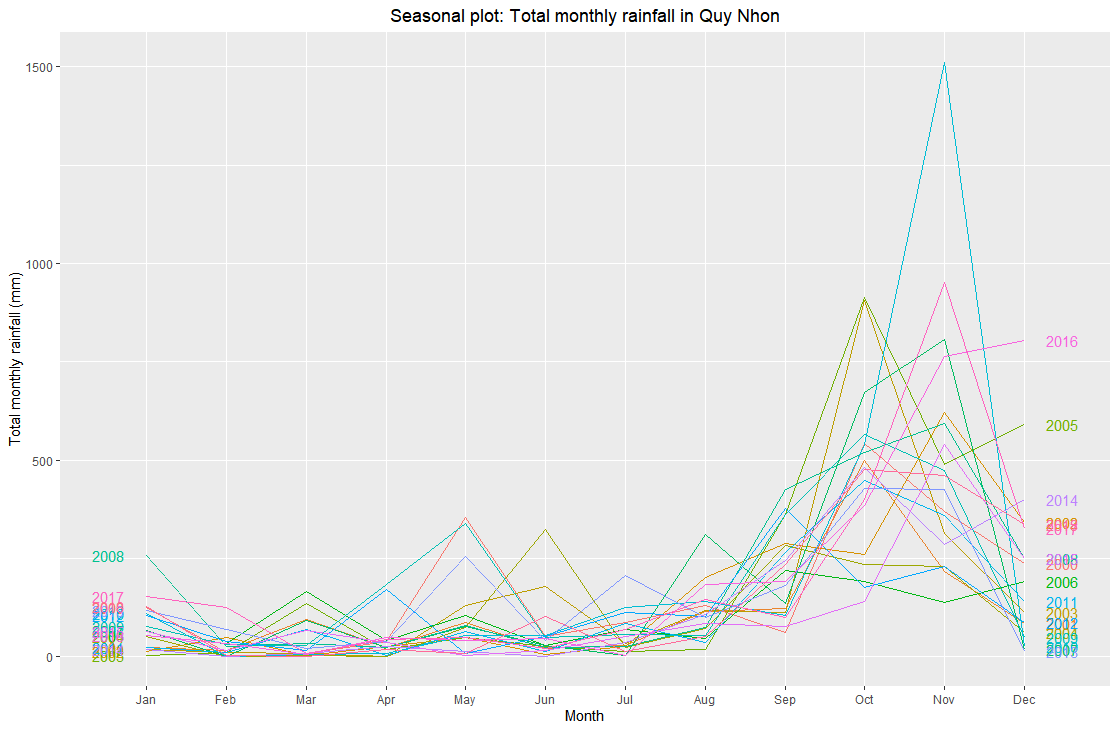
\includegraphics[width=1\linewidth,height=7.7cm]{anh/V2}
	\vskip-4mm 
	\caption{Đồ thị theo mùa của dữ liệu lượng mưa Quy Nhơn}  
	\label{V2}
\end{figure}
Tiếp theo, chúng tôi sẽ biểu diễn lượng mưa trung bình tại các tháng từ tháng 1/2000 đến tháng 12/2018. Kết quả của dòng lệnh được hiển thị trong hình \ref{V4}.
\begin{lstlisting}
ggsubseriesplot(rainfall) +
theme(plot.title = element_text(hjust = 0.5)) + 
ylab("Total monthly rainfall (mm)") +
ggtitle("Seasonal subseries plot: Total monthly rainfall in Quy Nhon")
\end{lstlisting}
\begin{figure}[!htb]
	\centering
	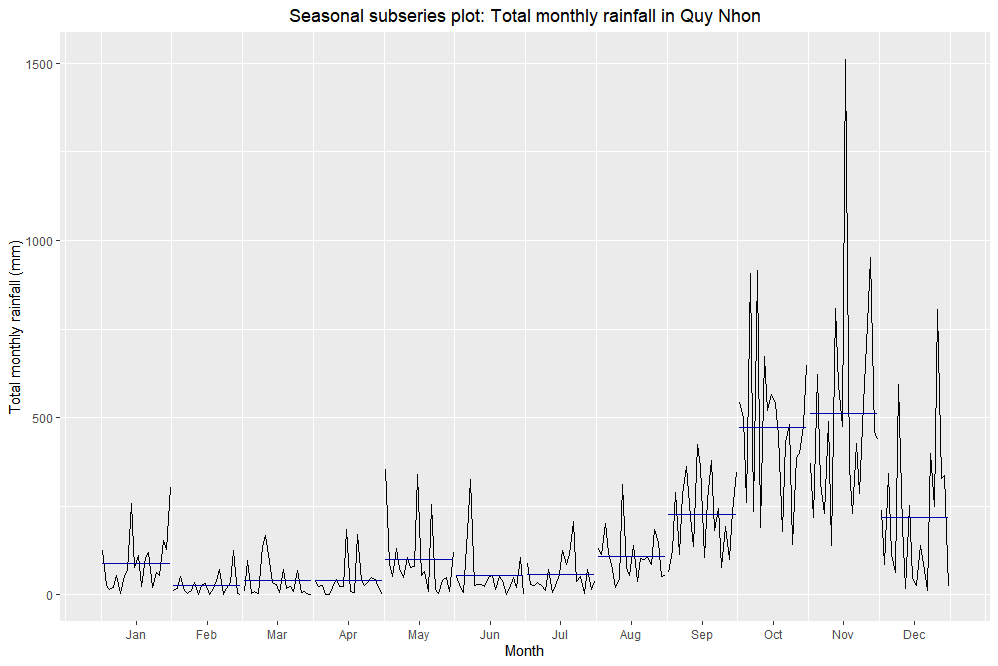
\includegraphics[width=1\linewidth,height=7.7cm]{anh/V4}
	\vskip-4mm 
	\caption{Đồ thị biểu thị lượng mưa trung bình tại các tháng}  
	\label{V4}
\end{figure}
Khí hậu tại Quy Nhơn có 2 mùa rõ rệt là mùa mưa (từ tháng 9 đến tháng 12) và mùa khô (từ tháng 1 đến tháng 8). Quan sát hình \ref{V2} và hình \ref{V4}, chúng ta thấy lượng mưa tại trạm quan trắc Quy Nhơn tập trung vào tháng 9 đến tháng 12, lượng mưa lớn nhất là vào tháng 11. Lượng mưa trung bình vào các tháng mùa mưa ít có biến động nhiều. Điều này thuận lợi để mô hình hóa ARIMA theo mùa.

\subsection{\label{lmqn}Dự báo lượng mưa hàng tháng tại trạm quan trắc Quy Nhơn}
Chúng tôi sẽ chia tập dữ  liệu "train" và "test" để thực hiện việc mô hình hóa ARIMA theo mùa.\\
\begin{lstlisting}
train <- rainfall[1:216] %>% ts(start = c(2000,1), frequency = 12)
test <- rainfall[217:228] %>% ts(start = c(2018,1), frequency = 12)
\end{lstlisting}
\textbf{Bước 1: Kiểm tra tính dừng của tập "train"}\\
\begin{lstlisting}
autoplot(train) + ggtitle("Data monthly rainfall in Quy Nhon") + 
theme(plot.title = element_text(hjust = 0.5)) + 
xlab("Month_Year") +
ylab("Total monthly rainfall (mm)")
\end{lstlisting}
Từ việc chạy các lệnh trên, chúng ta được kết quả như hình \ref{V5}.
\begin{figure}[!htb]
	\centering
	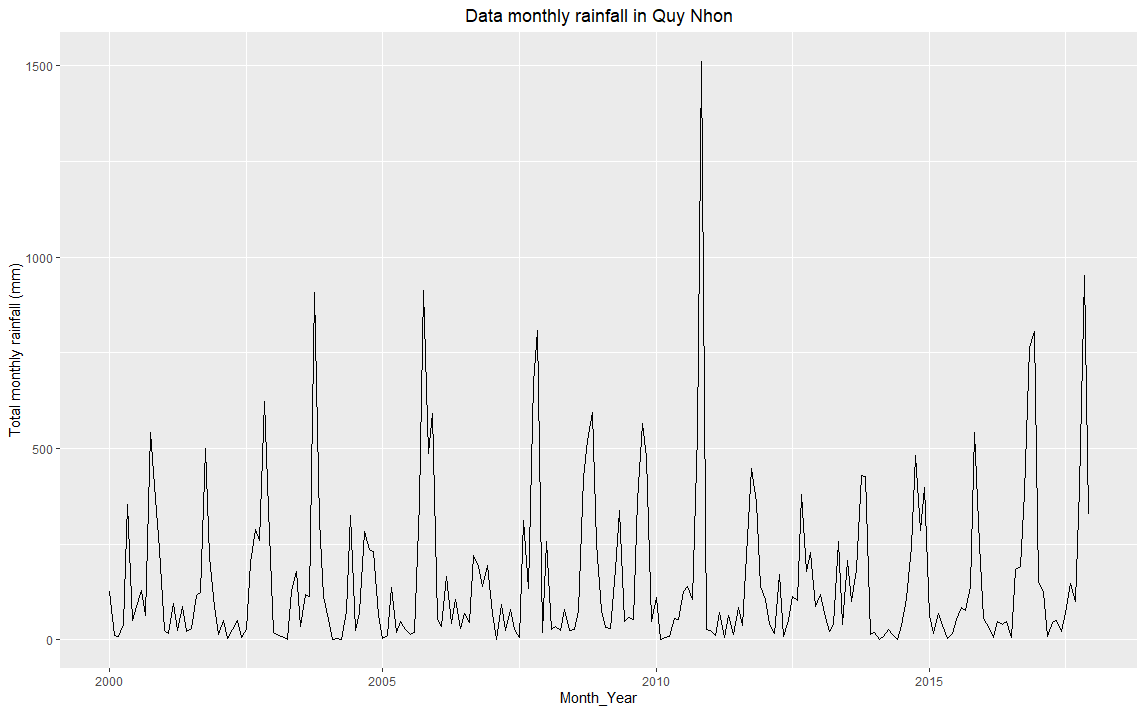
\includegraphics[width=1\linewidth,height=7.7cm]{anh/V5}
	\vskip-4mm 
	\caption{Đồ thị chuỗi thời gian dữ liệu tập "train" lượng mưa Quy Nhơn}  
	\label{V1}
\end{figure}
Chúng tôi xem xét các biện pháp tự tương quan (ACF) bằng cách sử dụng \lstinline{ggAcf(train)}. Ta được kết quả như hình \ref{V5}.
\begin{figure}[!htb]
	\centering
	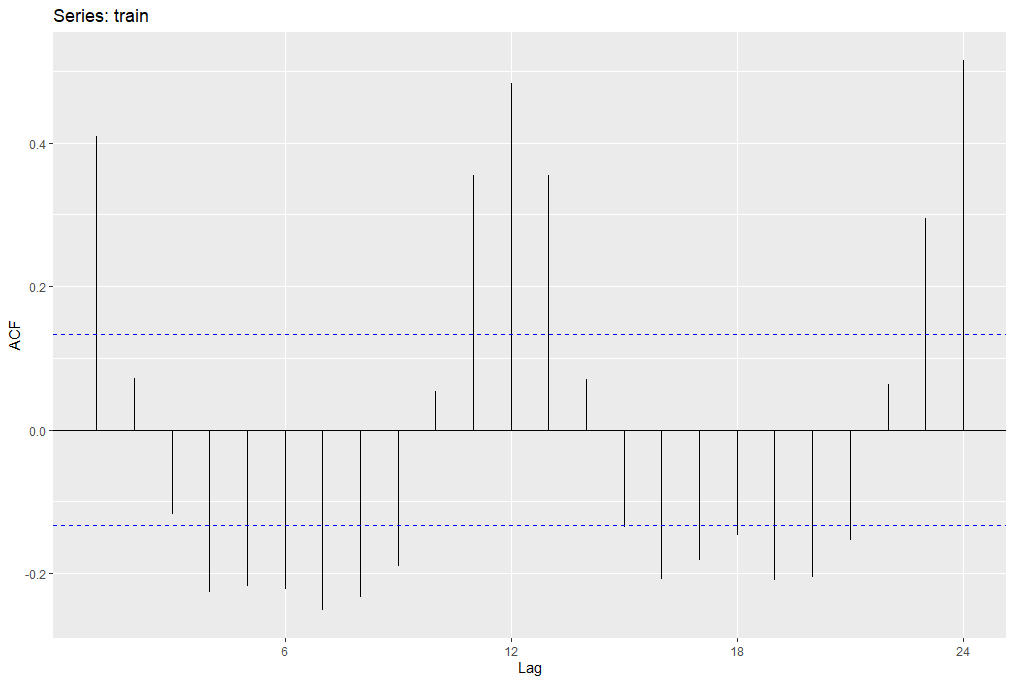
\includegraphics[width=1\linewidth,height=7.7cm]{anh/acfrainfall}
	\vskip-4mm 
	\caption{Đồ thị ACF của chuỗi thời gian đào tạo}  
	\label{V5}
\end{figure}
Chúng ta thấy đồ thị ACF có dạng hình \textit{sin} - dấu hiệu cho tính không dừng của tập "train". Quan sát hình \ref{V1} và \ref{V5}, chúng ta thấy chuỗi thời gian trong tập "train" không có tính ổn định.\\
\textbf{Bước 2: Chuyển chuỗi không dừng thành chuỗi dừng}\\
Cần lưu ý rằng, việc lấy sai phân trước hay lấy sai phân theo mùa trước đều cho kết quả cuối cùng như nhau mà không phụ thuộc vào thứ tự thực hiện. Tuy nhiên, chúng ta ưu tiên lấy sai phân theo mùa trước vì nó có thể giúp chuỗi có tính dừng ngay mà không cần phải lấy sai phân bậc 1. Hàm \lstinline{ndiffs} và \lstinline{nsdiffs} lần lượt gợi ý cho chúng ta bậc của sai phân và sai phân theo mùa hợp lý nhất.
\begin{lstlisting}
ndiffs(train)
##  0
nsdiffs(train)
##  1
\end{lstlisting}
Từ kết quả trên, chúng ta sẽ lấy sai phân bậc một theo mùa và vẽ đồ thị biểu diễn kết quả lấy sai phân bằng lệnh sau
\begin{lstlisting}
train %>% diff(lag=12) -> train.diff.rainfall
train.diff.rainfall %>% ggtsdisplay()
\end{lstlisting}
\begin{figure}[!htb]
	\centering
	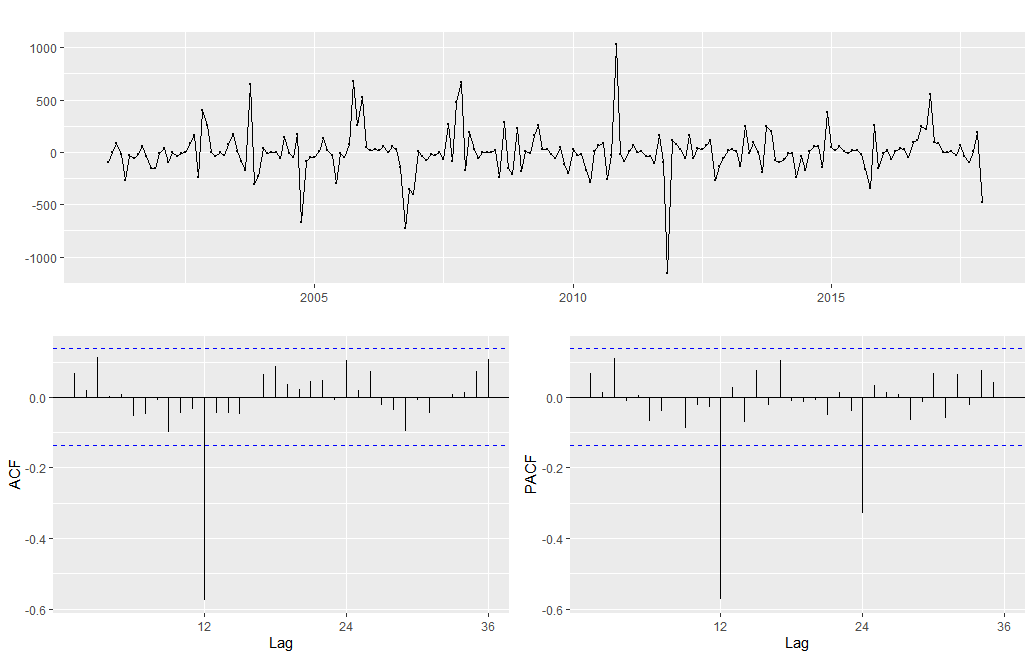
\includegraphics[width=1\linewidth,height=7.7cm]{anh/V6}
	\vskip-4mm 
	\caption{Đồ thị chuỗi thời gian đào tạo sau khi lấy sai phân bậc một theo mùa}  
	\label{V6}
\end{figure}
Quan sát đồ thị \ref{V6}, chúng ta thấy chuỗi đã có tính dừng sau khi lấy sai phân theo mùa. Chúng ta sẽ thực hiện thêm một bài kiểm tra về tính dừng bằng thử nghiệm ADF. 
\begin{lstlisting}
adf.test(train.diff.rainfall, alternative = "stationary")
##	  Augmented Dickey-Fuller Test
## data:  train.diff.rainfall
## Dickey-Fuller = -5.5754, Lag order = 5, p-value = 0.01
## alternative hypothesis: stationary
\end{lstlisting}
Với $p-value = 0.01 < 0.05$, kết hợp với các đồ thị quan sát ở trên, chúng ta kết luận chuỗi dữ liệu tập "train" sau khi lấy sai phân bậc 1 theo mùa đã có tính dừng.\\
\textbf{Bước 3: Chọn mô hình thích hợp từ đồ thị ACF và PACF}\\
Quan sát hình \ref{V6}, trong đồ thị ACF, sự tăng đột biến đáng kể tại $lag$ 12 nên có thể chỉ ra thành phần theo mùa MA(1) và không có sự biến động đáng kể nào tại các $lag$. Do đó, ACF gợi ý cho chúng ta một mô hình ARIMA(0,0,0)(0,1,1)$_{12}$ ($AICc=2648.02$). Tương tự, dựa vào biểu đồ PACF, sự tăng đột biến tại các $lag$ 12 và $lag$ 24 cho chúng ta thấy thành phần theo mùa MA(2). Điều này gợi ý cho chúng ta một mô hình ARIMA(0,0,0)(0,1,2)$_{12}$ ($AICc=2648.89$). Chúng tôi chọn mô hình  ARIMA(0,0,0)(0,1,1)$_{12}$ (AICc nhỏ hơn) là mô hình thích hơp ban đầu.\\
\textbf{Bước 4: Khớp và chọn mô hình tốt nhất}\\
Chúng ta sẽ tiến hành khớp (fit) mô hình ARIMA(0,0,0)(0,1,1)$_{12}$ bằng thuật toán Hyndman-Khandakar (2008).
\begin{table}[!h]
	\caption{Fit mô hình ARIMA theo mùa}
	\label{fit_rainfall}
	\centering
	\fontsize{6}{10}\selectfont
	\begin{tabular}[t]{lrrrrrr}
		\toprule
		STT	& SARIMA Models & AICc & RMSE train\\
		\midrule
		\rowcolor{gray!6}  1 & $ARIMA(0,0,0)(0,1,1)_{12}$ & 2650.64  & 146.5263\\
		2 & $ARIMA(1,0,0)(0,1,0)_{12}$ & 2649.27 & 146.3757\\
		\rowcolor{gray!6}  3 & $ARIMA(0,0,1)(0,1,1)_{12}$ & 2649.26  & 146.3721\\
		4 & $ARIMA(0,0,0)(1,1,1)_{12}$ & 2648.60 & 146.8532\\
		\rowcolor{gray!6} 5  & $ARIMA(0,0,0)(0,1,2)_{12}$ & 2648.89 & 146.8414\\
		6 & $ARIMA(1,0,0)(2,1,1)_{12}$ & 2648.02 & 145.6458\\
        \rowcolor{gray!6} 7  & $ARIMA(1,0,1)(0,1,1)_{12}$ & 2651.02 & 146.3285\\
        8  & $ARIMA(0,0,0)(1,1,2)_{12}$ & 2650.42 & 146.7120\\
		\bottomrule
	\end{tabular}
\end{table}
Từ kết quả được mô tả trong bảng \ref{fit_rainfall}, chúng tôi chọn mô hình $ARIMA(1,0,0)(2,1,1)_{12}$ (AICc và RMSE nhỏ nhất) là tốt nhất.\\
\textbf{Bước 5: Kiểm tra phần dư từ mô hình được chọn}\\
Phần dư của mô hình được vẽ trong hình \ref{V7}. Tất cả các spike đều nằm trong giới hạn, vì vậy phần dư là nhiễu trắng. Thử nghiệm Ljung-Box cũng cho thấy phần dư không còn tự tương quan. Chúng tôi đã xây dựng một mô hình ARIMA theo mùa thỏa mãn các kiểm tra cần thiết và sẵn sàng để dự báo.\\
\begin{lstlisting}
best.md.rainfall <- Arima(train, order=c(1,0,0), seasonal=c(2,1,1))
checkresiduals(best.md.rainfall)

##          	Ljung-Box test

##    data:  Residuals from ARIMA(1,0,0)(2,1,1)[12]
##    Q* = 8.8729, df = 20, p-value = 0.9843
##    Model df: 4.   Total lags used: 24
\end{lstlisting}
\begin{figure}[!htb]
	\centering
	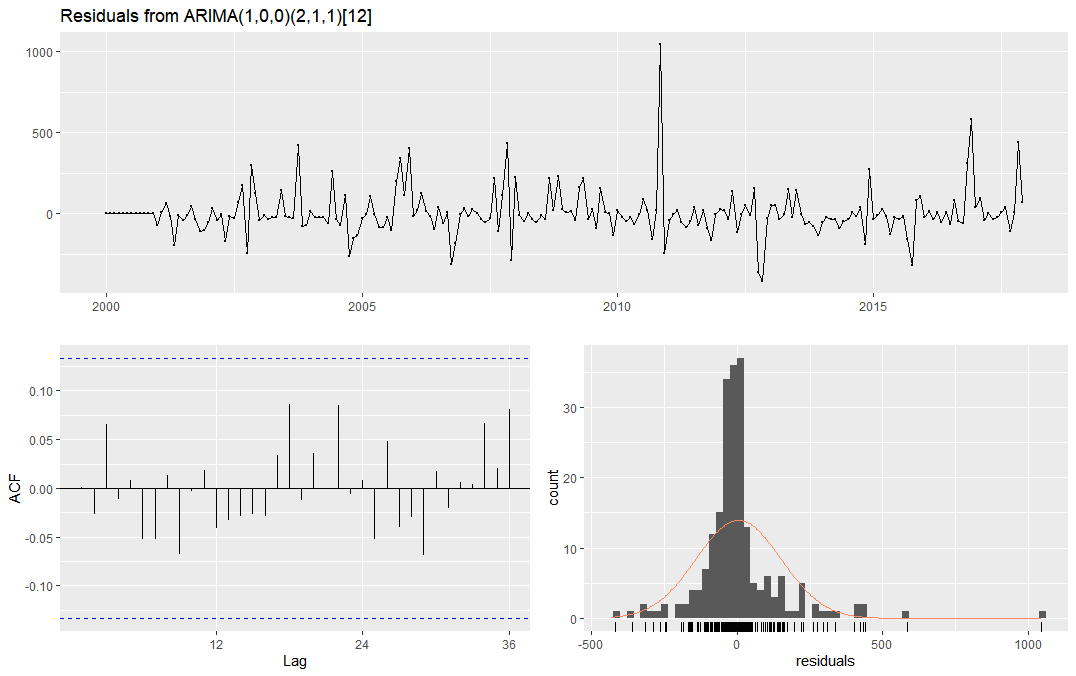
\includegraphics[width=1\linewidth,height=7.7cm]{anh/V7}
	\vskip-4mm 
	\caption{Đồ thị kiểm tra phần dư từ mô hình đào tạo}  
	\label{V7}
\end{figure}
\textbf{Bước 6: Đánh giá sai số từ mô hình và dự báo}\\
Tiếp theo, chúng tôi tiến hành đánh giá sai số từ mô hình $ARIMA(1,0,0)(2,1,1)_{12}$ bằng cách dự báo cho 12 tháng tiếp theo và so sánh với 12 tháng thực tế trên tập "test". Các câu lệnh được thực hiện như sau
\begin{lstlisting}
test.fc.rainfall <- forecast(best.md.rainfall, h = 12) 
vector.color <- c("purple3", "blue", "green", "red")
autoplot(test.fc.rainfall) +
autolayer(test.fc.rainfall$mean, series="Forecast") +
autolayer(fitted(best.md.rainfall), series='Fitted') + 
autolayer(train, series = "Train") +
autolayer(test, series="Test") + 
xlab("Observation [Monthlys]") +
ylab("Monthly Rainfall [mm]") +
guides(colour=guide_legend(title="Data series"), 
fill=guide_legend(title="Prediction interval"))+
scale_color_manual(values= vector.color)
\end{lstlisting}
\begin{figure}[!htb]
	\centering
	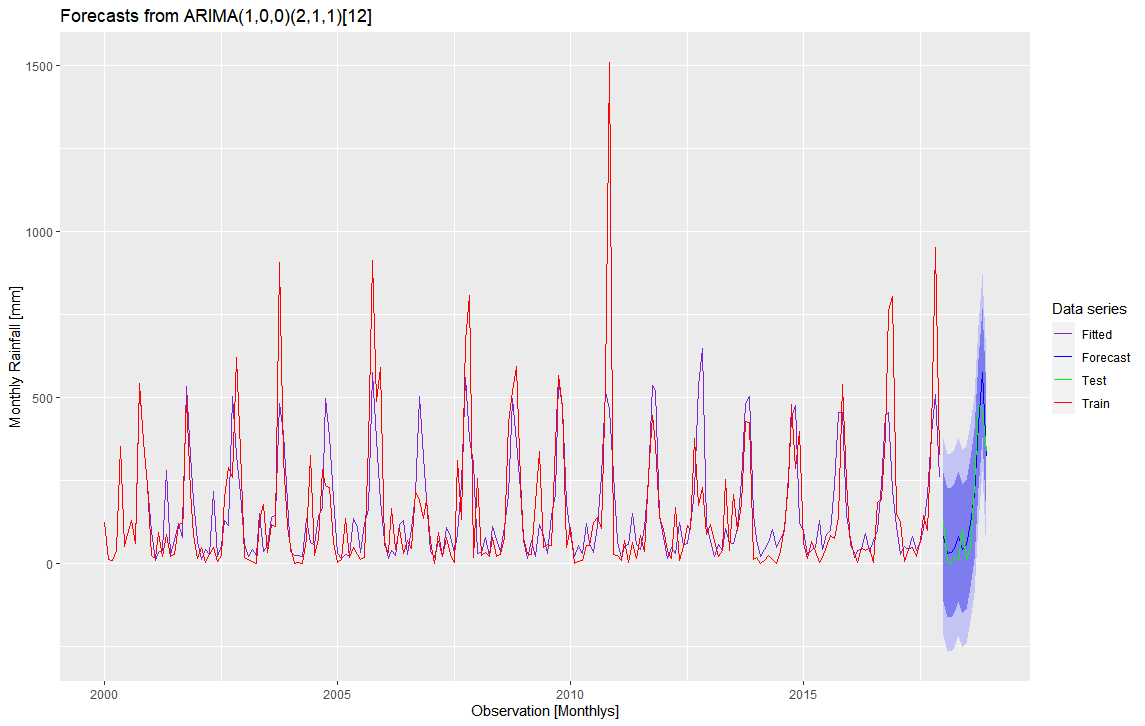
\includegraphics[width=1\linewidth,height=7.7cm]{anh/V8}
	\vskip-4mm 
	\caption{Đồ thị đối sánh kết quả thực và dự báo cho lượng mưa}  
	\label{V8}
\end{figure}
\begin{table}[!h]	
	\caption{Đối sánh giữa kết quả dự báo và tập test cho lượng mưa}
	\label{test_fc}
	\centering
	\fontsize{6}{8}\selectfont
	\begin{tabular}[t]{lrrrrrrr}
		\toprule
		&Point Actual(A) & Point Forecast (F)& Lo 80 & Hi 80 & Lo 95 & Hi 95& $\dfrac{A-F}{A}.100\%$\\
		\midrule
		\rowcolor{gray!6}  Jan 2018 & 128.6 & 81.81485 & -112.37714 & 276.0068 & -215.17616 & 378.8059 & 36\%\\
		Feb 2018 & 2.8 & 32.32366 & -162.30622 & 226.9535 & -265.33706 & 329.9844 & -1054\%\\
		\rowcolor{gray!6}  Mar 2018 & 1.6 & 34.07819 & -160.55367 & 228.7101 & -263.58555 & 331.7419 & -2029\%\\
		Apr 2018 & 20.0 & 46.95980 & -147.67208 & 241.5917 & -250.70397 & 344.6236 & -134\%\\
		\rowcolor{gray!6}  May 2018 & 9.4 & 82.40952 & -112.22235 & 277.0414 & -215.25424 & 380.0733 & -776\%\\
		\addlinespace
		Jun 2018 & 103.7 & 44.63459 & -149.99728 & 239.2665 & -253.02917 & 342.2984 & 56\%\\
		\rowcolor{gray!6}  Jul 2018 & 14.0 & 57.38414 & -137.24773 & 252.0160 & -240.27962 & 355.0479 & -309\%\\
		Aug 2018 & 51.1 & 122.92861 & -71.70327 & 317.5605 & -174.73515 & 420.5924 & -140\%\\
		\rowcolor{gray!6}  Sep 2018 & 235.5 & 209.18078 & 14.54891 & 403.8127 & -88.48298 & 506.8445 & 11\%\\
		Oct 2018 & 476.7 & 420.49951 & 225.86764 & 615.1314 & 122.83575 & 718.1633 & 11\%\\
		\addlinespace
		\rowcolor{gray!6}  Nov 2018 & 462.0 & 574.92124 & 380.28937 & 769.5531 & 277.25748 & 872.5850 & -24\%\\
		Dec 2018 & 337.9 & 321.89014 & 127.25849 & 516.5218 & 24.22672 & 619.5536 & 4\%\\
		\bottomrule
	\end{tabular}
\end{table}
Quan sát bảng \ref{test_fc} và hình \ref{V8}, chúng ta thấy các tháng thuộc mùa khô (từ tháng 1 đến tháng 8) có sự chênh lệnh lớn bởi vì khí hậu đang thay đổi thất thường và các nhà dự báo thời tiết cũng khó dự báo chính xác được. Sai số lớn vào mùa khô có thể được giải thích như sau:
\begin{itemize}
	\item Theo \cite{22}, sự thay đổi của hệ thống khí hậu làm gia tăng biến động của khí hậu trên tất cả quy mô thời gian. Một số quá trình xảy ra trong khoảng thời gian ngắn, như sự phát triển của hệ thống synop trong khí quyển là một trong những nguyên nhân dẫn đến sai số dự báo mùa. Tuy nhiên, sự thay đổi chậm của hệ thống khí hậu lại là nguồn gốc cơ bản cho phép dự báo khí hậu mùa. Nguyên nhân của sự thay đổi này bao gồm sự thay đổi trong khoảng thời gian dài của đại dương, hệ thống tương tác đại dương-khí quyển và các thành phần khác như băng biển, điều kiện bề mặt đất, độ che phủ của tuyết ...
	\item El Nino và Dao động Nam (SO) được xem là nhân tố tác động lớn nhất đến biến đổi khí hậu, trong đó có lượng mưa. Walker (1924) đã phát hiện ra dao động của khí áp quy mô lớn, từ năm này qua năm khác ở 2 phía Đông và Tây của khu vực xích đạo Thái Bình Dương (Tahiti và Darwin) và được gọi là Dao động Nam. Hơn 40 năm sau, trong công trình nghiên cứu của Jacob Bjerknes (1969) thừa nhận có sự quan hệ chặt chẽ giữa Dao động Nam và sự thay đổi về nhiệt độ bề mặt nước biển trên khu vực Xích Đạo đông Thái Bình Dương. Mối quan hệ này thể hiện sự tương tác giữa đại dương và khí quyển mà biểu hiện của nó chính là hiện tượng ENSO (El Nino–Southern Oscillation). ENSO được dùng để chỉ cả 2 hai hiện tượng El Nino, La Nina và có liên quan với Dao động Nam. ENSO là nhân tố ảnh hưởng lớn nhất đến các dao động khí hậu hàng năm, chính sự kết hợp này là nguồn gốc chính sinh ra dị thường về nhiệt độ và lượng mưa trên phạm vi toàn cầu \cite{22, 23, 24}.
\end{itemize}
Tuy nhiên, các giá trị dự báo cho mùa mưa (tháng 9 đến tháng 12) cho kết quả sai số rất thấp. Điều này phù hợp với đặc điểm lượng mưa tại Quy Nhơn. Do đó, mô hình ARIMA(1,0,0)(2,1,1)$_{12}$ có thể dùng dự báo lượng mưa tại Quy Nhơn. Chúng tôi tiến hành dự báo lượng mưa theo tháng cho 2 năm tiếp theo ở Quy Nhơn.
\begin{lstlisting}
fit.md <- Arima(rainfall, order=c(1,0,0), seasonal=c(2,1,1))
fit.md %>% forecast(h=24) %>% autoplot()
\end{lstlisting}
\begin{table}[!h]
	\caption{Dự báo lượng mưa hàng tháng cho 2 năm tiếp theo ở Quy Nhơn}
	\label{kqrainfall}
	\centering
	\fontsize{6}{8}\selectfont
	\begin{tabular}[t]{lrrrrr}
		\toprule
		& Point Forecast & Lo 80 & Hi 80 & Lo 95 & Hi 95\\
		\midrule
		\rowcolor{gray!6}  Jan 2019 & 91.76578 & -96.60397 & 280.1355 & -196.32090 & 379.8525\\
		Feb 2019 & 42.27684 & -146.48860 & 231.0423 & -246.41498 & 330.9687\\
		\rowcolor{gray!6}  Mar 2019 & 33.84519 & -154.92190 & 222.6123 & -254.84917 & 322.5396\\
		Apr 2019 & 43.94335 & -144.82376 & 232.7105 & -244.75103 & 332.6377\\
		\rowcolor{gray!6}  May 2019 & 83.59559 & -105.17151 & 272.3627 & -205.09878 & 372.2900\\
		\addlinespace
		Jun 2019 & 46.60968 & -142.15743 & 235.3768 & -242.08470 & 335.3041\\
		\rowcolor{gray!6}  Jul 2019 & 61.58513 & -127.18198 & 250.3522 & -227.10925 & 350.2795\\
		Aug 2019 & 116.15631 & -72.61080 & 304.9234 & -172.53807 & 404.8507\\
		\rowcolor{gray!6}  Sep 2019 & 198.88576 & 10.11865 & 387.6529 & -89.80862 & 487.5801\\
		Oct 2019 & 434.81604 & 246.04893 & 623.5831 & 146.12166 & 723.5104\\
		\addlinespace 
		\rowcolor{gray!6}  Nov 2019 & 592.95521 & 404.18811 & 781.7223 & 304.26084 & 881.6496\\
		Dec 2019 & 260.07814 & 71.31136 & 448.8449 & -28.61573 & 548.7720\\
		\rowcolor{gray!6}  Jan 2020 & 89.25500 & -99.61077 & 278.1208 & -199.59027 & 378.1003\\
		Feb 2020 & 27.27827 & -161.58825 & 216.1448 & -261.56814 & 316.1247\\
		\rowcolor{gray!6}  Mar 2020 & 31.56637 & -157.30015 & 220.4329 & -257.28005 & 320.4128\\
		\addlinespace
		Apr 2020 & 40.21528 & -148.65124 & 229.0818 & -248.63113 & 329.0617\\
		\rowcolor{gray!6}  May 2020 & 75.65715 & -113.20936 & 264.5237 & -213.18926 & 364.5036\\
		Jun 2020 & 58.20946 & -130.65706 & 247.0760 & -230.63695 & 347.0559\\
		\rowcolor{gray!6}  Jul 2020 & 53.28597 & -135.58055 & 242.1525 & -235.56044 & 342.1324\\
		Aug 2020 & 102.82699 & -86.03953 & 291.6935 & -186.01943 & 391.6734\\
		\addlinespace
		\rowcolor{gray!6}  Sep 2020 & 214.99832 & 26.13180 & 403.8648 & -73.84809 & 503.8447\\
		Oct 2020 & 445.11325 & 256.24673 & 633.9798 & 156.26684 & 733.9597\\
		\rowcolor{gray!6}  Nov 2020 & 534.54059 & 345.67407 & 723.4071 & 245.69418 & 823.3870\\
		Dec 2020 & 265.01471 & 76.14849 & 453.8809 & -23.83125 & 553.8607\\
		\bottomrule
	\end{tabular}
\end{table}
\begin{figure}[!htb]
	\centering
	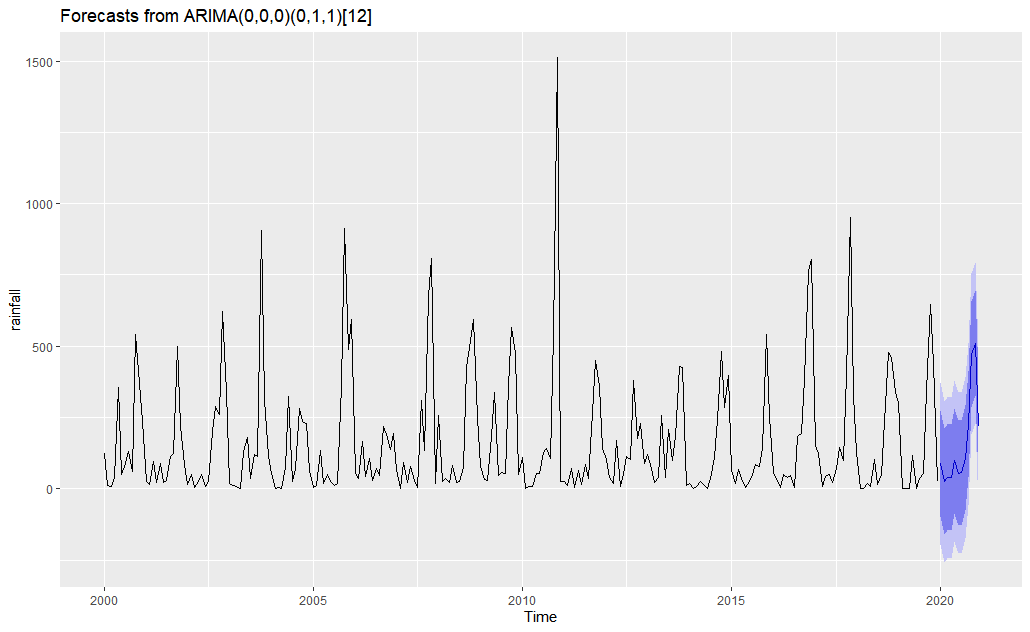
\includegraphics[width=1\linewidth,height=7.7cm]{anh/V9}
	\vskip-4mm 
	\caption{Đồ thị dự báo lượng mưa theo tháng từ mô hình ARIMA(0,0,0)(0,1,1)$_{12}$}  
	\label{V9}
\end{figure}
Quan sát kết quả dự báo tại bảng \ref{kqrainfall}, chúng ta thấy nhìn chung lượng mưa tại các tháng không thay đổi nhiều so với năm 2018. Điều này là một tín hiệu tốt cho thấy biến đổi khí hậu sẽ không lớn vào 2 năm tiếp theo. Từ kết quả dự báo này, chúng tôi hy vọng sẽ giúp ích trong việc hoạch định và điều tiết hệ thống tài nguyên nước.
\section{Webstie Dashboard COVID-19}
Trong khi dịch COVID-19 đang diễn ra, rất nhiều nhóm nghiên cứu trên thế giới tìm cách góp phần chuyên môn vào việc kiểm soát dịch. Không chỉ trong chuyên ngành dịch tễ học, mà rất nhiều chuyên gia từ các chuyên ngành khác nhau cũng tham gia trực tiếp hay gián tiếp. Điển hình như giới miễn dịch học, kinh tế, toán và thống kê, engineering,... Nhằm góp phần vào việc kiểm soát dịch, chúng tôi đã tạo ra một website hỗ trợ quan sát xu hướng dịch bệnh COVID-19 cho từng quốc gia bằng mô hình ARIMA. Trang web của chúng tôi chạy trên nền tảng R kết hợp với Shinyapp để tạo một bảng điều khiển và theo dõi xu hướng dịch COVID-19 trên toàn thế giới.
Link: \url{https://nguyenquocduong.shinyapps.io/NCKH}.\\
\subsection*{Mô tả trang web:}
Trang web cập nhật dữ liệu một cách tự động từ \url{https://github.com/CSSEGISandData/COVID-19}. Website có 4 tag lần lượt là:
\begin{itemize}
	\item Overiew: Trong tag này, chúng tôi cho hiển thị tổng số ca nhiễm, tổng số ca phục hồi, tổng số ca tử vong trên toàn thế giới và bảng chi tiết cho từng quốc gia.
	\item Trend Using ARIMA Model: Trong tag này, chúng tôi sử dụng hàm "auto.arima" để đưa ra xu hướng dịch bệnh cho từng quốc gia với 3 tùy chọn là confirmed, deaths, recovered.
	\item About: Thông tin về website
\end{itemize}
Từ ứng dụng này, chúng tôi có thể tạo ra một trang web tương tự để theo dõi và phân tích các bệnh cụ thể tại Việt Nam.

\section{So sánh mô hình ARIMA với mô hình NNAR}
Trong phần này, chúng tôi so sánh mô hình ARIMA và \textit{mô hình mạng noron tự hồi quy NNAR (Neural Retwork Auto-Regression)} trên tập dữ liệu lượng mưa hàng tháng tại trạm quan trắc Quy Nhơn dựa vào các thước đo sai số.
\subsection*{Tổng quan về mô hình NNAR}

Mạng neural nhân tạo hay thường gọi ngắn gọn là mạng noron (\textit{Artificial Neural network - ANN hay Neural Network}) là một mô hình toán học hay mô hình tính toán được xây dựng dựa trên các mạng noron sinh học. Nó gồm có một nhóm các noron nhân tạo (nút) nối với nhau, và xử lý thông tin bằng cách truyền theo các kết nối và tính giá trị mới tại các nút (cách tiếp cận connectionism đối với tính toán). Các thông tin này được hiển thị trong hình \ref{V7}. Trong nhiều trường hợp, mạng noron nhân tạo là một hệ thống thích ứng (adaptive system) tự thay đổi cấu trúc của mình dựa trên các thông tin bên ngoài hay bên trong chảy qua mạng trong quá trình học.
\begin{figure}[!htb]
	\centering
	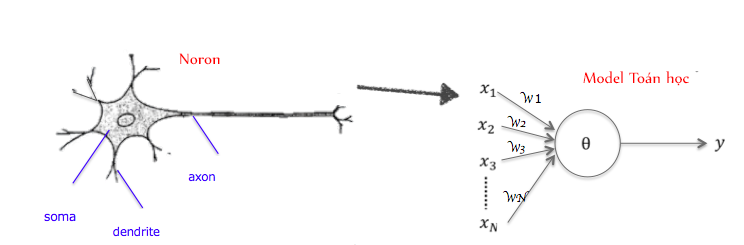
\includegraphics[width=1\linewidth,height=7.7cm]{anh/noron}
	\vskip-4mm 
	\caption{Mô tả mạng noron}  
	\label{V7}
\end{figure}
Với dữ liệu chuỗi thời gian, các giá trị bị trễ của chuỗi thời gian có thể được sử dụng làm đầu vào cho mạng thần kinh, giống như chúng ta đã sử dụng các giá trị bị trễ trong mô hình ARIMA. Chúng tôi gọi đây là mô hình mạng noron tự hồi quy hoặc mô hình NNAR.

Hàm tổ hợp tuyến tính có dạng tổng quát
\begin{align*}
y_t = a_t + \sum_{i =1}^{n}w_{i, t}x_t.
\end{align*}
Các tham số $a_t$ và $w_{i, t}$ được "học" từ dữ liệu và $x_t$ là các giá trị trễ (lagged values) của chuỗi thời gian. Các giá trị trọng số thường được hạn chế nhằm ngăn chúng trở nên quá lớn. Tham số mà hạn chế các trọng số thường được biết đến là \textit{tham số phân rã} (decay parameter) và nó thường được cho bằng 0.1. Ở thời điểm bắt đầu, các trọng số nhận giá trị ngẫu nhiêu và sau đó, sử dụng dữ liệu quan sát, chúng được cập nhật.

Trong tầng ẩn (hidden layer), khi đó $y_t$ được điều chỉnh với việc sử dụng một hàm phi tuyến, chẳng hạn hàm sigmoid
\begin{align*}
f(y_t) = \frac{1}{1+e^{-y_t}},
\end{align*}
để nhận được giá trị đầu vào cho tầng kế tiếp. Kĩ thuật này hướng tới việc làm giảm ảnh hưởng của các giá trị đầu vào cực lớn, do vậy giúp mạng lưới hoạt động tốt đối với các giá trị ngoại lai (outliers). 

Trong phần này, chúng tôi chỉ xem xét các mạng chuyển tiếp (feed-forward networks) có 1 tầng ẩn. Chúng tôi kí hiệu mô hình NNAR($p$, $k$), với $p$ đầu vào bị trễ và $k$ mút trong tầng ẩn.  Mô hình NNAR($p$, 0) tương đương với mô hình ARIMA($p$, 0, 0) nhưng không có các hạn chế lên tham số để đảm bảo tính ổn định.

Đối với dữ liệu có tính mùa vụ, ta có mô hình NNAR($p$, $P$, $k$)$_m$ tổng quát với các đầu vào là $(y_{t-1}, y_{t-2},\dots, y_{t-p}, y_{t-m}, y_{t-2m}, y_{t-Pm})$ và $k$ noron tầng ẩn. Mô hình NNAR($p$, $P$, 0)$_m$ là tương đương với mô hình ARIMA($p$, 0, 0)($P$, 0, 0)$_m$ nhưng không có các giới hạn về các tham số để đảm bảo tính dừng.

\textit{Hàm $nnetar()$ giúp chọn mô hình NNAR($p$, $P$, $k$)$_m$ phù hợp}. Nếu các giá trị của $p$ và $P$ không được chỉ định thì chúng được chọn một cách tự động. Đối với chuỗi thời gian không theo mùa, số các lag được tối ưu (dựa theo AIC) cho mô hình AR($p$) tuyến tính. Đối với chuỗi thời gian có tính mùa, các giá trị mặc định $P=1$ và $p$ được chọn từ mô hình tuyến tính tốt nhất phù hợp với dữ liệu được điều chỉnh theo mùa. Nếu $k$ không được chỉ định, ta đặt $k = (p + P + 1)/2$ (làm tròn đến số nguyên gần nhất).

Để dự báo trước một bước, chúng ta sử dụng các dữ liệu đầu vào có sẵn. Đối với dự báo trước hai bước, chúng ta sử dụng dự báo một bước và dữ liệu lịch sử làm đầu vào. Quá trình này tiến hành cho đến khi chúng ta đã tính toán được tất cả các dự báo cần thiết.

\subsection*{So sánh ARIMA và NNAR trên tập dữ liệu lượng mưa Quy Nhơn}

Tập dữ liệu được chúng tôi sử dụng để đánh giá mô hình là dữ liệu lượng mưa tại trạm quan trắc Quy Nhơn như trong phần \ref{lmqn}. Chúng tôi sử dụng hàm nner() để tìm ra mô hình NNAR phù hợp nhất. Tương tự, hàm auto.arima dùng để đưa ra mô hình ARIMA phù hợp nhất.\\
\begin{lstlisting}
###########################################################
# NNAR MODEL

model.nnar <- nnetar(train)
fit1 <- model.nnar %>% forecast(h = 12, PI = TRUE) %>%
accuracy(rainfall)
fit1[,c("RMSE","MAE","MASE")]

## Model:  NNAR(1,1,2)[12] 

## Average of 20 networks, each of which is a 2-2-1 network with 9 weights options were - linear output units, sigma^2 estimated as 26867

##                    RMSE        MAE        MASE
## Training set  163.9116    105.6931   0.8598967
## Test set       119.7967   103.0955   0.8387630   

###########################################################

# ARIMA MODEL

model.arima <- auto.arima(train)
fit2 <- model.arima %>% forecast(h = 12) %>%
accuracy(rainfall)
fit2[,c("RMSE","MAE","MASE")]

## ARIMA(1,0,0)(2,1,1)[12] 

## Coefficients:
##          ar1     sar1    sar2     sma1
##       0.0672  -0.0526  0.1004  -0.8817
## s.e.  0.0682   0.0929  0.0876   0.0937

## sigma^2 estimated as 22910:  log likelihood=-1320.17

##                     RMSE        MAE        MASE
## Training set 145.64577     84.20232  0.6850522
## Test set        55.94754   49.54044  0.4030505   
\end{lstlisting}
Từ kết quả trên, chúng ta thấy rằng các thước đo sai số RMSE, MAE, MASE trên tập "train" và tập "test" của mô hình ARIMA đều thấp hơn rất nhiều so với các sai số tương ứng trên mô hình NNAR. Do đó, đối với tập dữ liệu này, mô hình ARIMA thể hiện khả năng dự báo tốt hơn mô hình NNAR. Vì lí do thời gian còn hạn chế, chúng tôi chỉ so sánh giữa ARIMA và NNAR. Trong thời gian tới, chúng tôi sẽ mở rộng so sánh thêm với một số mô hình hiện đại như LSTM (Long Short Term Memory), ARIMA-LSTM, ARIMA-ANN, \dots
\section*{Kết luận chương 2}
Trong Chương 2, chúng tôi đã sử dụng các gói lệnh trong R để phân tích tổng quan dữ liệu COVID-19, dự báo số ca nhiễm mới tại Mỹ, dự báo số ca tử vong mới ở Italy và dự báo lượng mưa hàng tháng tại trạm quan trắc Quy Nhơn. Qua từng bộ dữ liệu được phân tích, chúng tôi thấy được mô hình ARIMA đã cho khả năng dự báo rất tốt. Hơn nữa, chúng tôi đã khai thác rất hiệu quả tính năng của R để xây dựng được website Dashboard COVID-19 nhằm góp phần vào công cuộc chống đại dịch toàn cầu.
\chapter*{Thảo luận}
\section*{Những mặt thuận lợi và hạn chế của mô hình ARIMA}
Dự báo chính xác là một nhiệm vụ quan trọng nhưng thường là khó khăn đối với các nhà hoạch định chính sách trong nhiều lĩnh vực. Mặc dù có rất nhiều mô hình được ứng dụng trong việc dự báo nhưng mỗi mô hình đều có thuận lợi và hạn chế riêng. Do đó, chúng ta cần nắm bắt được những điểm thuận lợi và hạn chế của mô hình được đưa ra.
\subsection*{Những điểm thuận lợi khi sử dụng ARIMA}
\begin{itemize}
	\item ARIMA là một trong những mô hình tuyến tính phổ biến nhất trong dự báo chuỗi thời gian đã được áp dụng rộng rãi trong thập kỷ qua.
	\item ARIMA phát huy thế mạnh trong việc sử dụng để dự báo tài chính, chứng khoán, kinh tế lượng, khí tượng thủy văn, ...
	\item ARIMA thích hợp cho các bài toán dự báo ngắn hạn.
	\item Hơn nữa, ARIMA còn là nền tảng để xây dựng các mô hình lai phù hợp với từng loại dữ liệu cụ thể và cho kết quả chính xác hơn như ARIMA-ANN, ARIMA-LSTM, ARIMAX,...
\end{itemize}
\subsection*{Những mặt hạn chế khi sử dụng ARIMA}
\begin{itemize}
	\item Trong ARIMA, một cấu trúc tương quan tuyến tính được giả định giữa các giá trị trong chuỗi thời gian. Do đó, đối với dữ liệu có tính chất phi tuyến thì mô hình ARIMA không phát hiện được. 
	\item Các giá trị trong tương lai được dự báo phụ thuộc vào quá khứ nên đối với bài toán dự báo dài hạn, việc lựa chọn ARIMA là không phù hợp.
\end{itemize}
\chapter*{Kết luận và kiến nghị}
Trong đề tài này, chúng tôi đã đạt được một số kết quả sau: 
\begin{itemize}
	\item[(1)] Tìm hiểu lý thuyết căn bản, quan trọng về chuỗi thời gian, hồi quy cổ điển với chuỗi thời gian và mô hình ARIMA.
	\item[(2)] Bước đầu đã nắm vững cách sử dụng các lệnh trong R để xây dựng mô hình ARIMA; hiểu và giải thích được kết quả đầu ra của mô hình ARIMA, cũng như nắm được kỹ năng về xử lý số liệu thô và kỹ năng vẽ hình, biểu đồ bằng phần mềm R.
	\item[(3)] Hơn nữa, chúng tôi đã xây dựng một website Dashboard COVID-19 nhằm theo dõi xu hướng dịch bệnh cho mỗi quốc gia bằng mô hình ARIMA với phần mềm R.
	\item[(4)] Đồng thời, trong quá trình làm phần ví dụ thực hành với R, chúng tôi đã có điều kiện tìm hiểu thêm nhiều kiến thức mới ở các lĩnh vực khác nhau như: dịch tễ học, y tế cộng đồng, khí tượng thủy văn, \dots.
\end{itemize}
Trong thời gian tới, chúng tôi mong muốn thực hiện các nghiên cứu về khoa học dữ liệu với R (data science, mô hình phân tích sống sót) trên số liệu thực gắn với lĩnh vực Y sinh, sức khỏe cộng đồng và đời sống kinh tế-xã hội của địa phương, trong nhiều lĩnh vực khác nhau, để có thể mang lại những ứng dụng thiết thực cho tỉnh Bình Định.

%%%%%% Lập phụ lục - Nguyễn Quốc Dương
\appendix
\chapter{Các định lý và thuật toán}
\section{Thuật toán Hyndman - Khandakar (2008)}
\begin{algo}\cite{3}\label{H} \textbf{Hyndman - Khandakar (2008)}\\
	\begin{itemize}
		\item Bước 1: Chúng ta chọn một trong 4 mô hình sau để bắt đầu.
		\begin{itemize}
			\item $ARIMA(2,d,2)$ nếu $m=1$ và $ARIMA(2,d,2)(1,D,1)_{12}$ nếu $m >1$.
			\item $ARIMA(0,d,0)$ nếu $m = 1$ và $ARIMA(0,d,0)(0,D,0)_{12}$ nếu $m >1$.
			\item $ARIMA(1,d,0)$ nếu $m = 1$ và $ARIMA(1,d,0)(1,D,0)_{12}$ nếu $m >1$.
			\item $ARIMA(0,d,1)$ nếu $m = 1$ và $ARIMA(0,d,1)(0,D,1)_{12}$ nếu $m >1$.
		\end{itemize}
		Nếu $d+D\leq1$ thì các mô hình này được khớp với $c\neq0$. Ngược lại, chúng ta sẽ khớp với $c=0$. Trong bốn mô hình này, chúng tôi chọn một mô hình có AICc nhỏ nhất. Gọi nó là mô hình hiện tại và kí hiệu $ARIMA(p,d,q)$ nếu $m=1$ hoặc $ARIMA(p,d,q)(P,D,Q)_m$ nếu $m>1$.\\
		\item Bước 2: Chúng tôi xem xét 13 biến thể trên mô hình hiện tại.
		\begin{itemize}
			\item điều chỉnh $p$, $q$, $P$ và $Q$ $\pm1$ so với mô hình hiện tại;
			\item điều chỉnh cả $p$ và $q$ $\pm1$ so với mô hình hiện tại;
			\item điều chỉnh cả $P$ và $Q$ $\pm1$ so với mô hình hiện tại;
			\item chọn nếu mô hình hiện tại có $c = 0$ hoặc loại trừ nếu mô hình hiện tại có $c\neq0$.
			Bất kỳ một mô hình nào được tìm thấy, nếu AIC của mô hình nhỏ hơn thì lập tức trở thành mô hình hiện tại mới và quá trình này lặp lại. Quá trình này kết thúc khi chúng ta không thể tìm thấy một mô hình gần với mô hình hiện tại với AIC thấp nhất. 
		\end{itemize}
	\end{itemize}
\end{algo}
%%%%%%%%%%%%
Thuật toán trả về một mô hình thích hợp và được chọn để dự báo.
\section{\label{TĐSS}Các thước đo đánh giá sai số dự báo}
Sai số dự báo là chênh lệch giữa giá trị thực tế và giá trị dự báo tương ứng $e_t = Y_t - \hat{Y_t}$. Trong đó, $Y_t$ là giá trị thực tế và $\hat{Y_t}$ là giá trị dự báo. Trong bài báo cáo này, chúng tôi sử dụng các thước đo sai số dự báo sau \cite{3,4}:
\begin{itemize}
\item Sai số bình phương trung bình (MSE - Mean Squared Error): 
$$MSE=\frac{1}{n}\sum_{t=1}^{n}(Y_t-\hat{Y_t})^2.$$

\item Căn của sai số bình phương trung bình (RMSE - Root Mean Squared Error):
$$RMSE=\sqrt{MSE}=\sqrt{\frac{1}{n}\sum_{t=1}^{n}(Y_t-\hat{Y_t})^2}  $$

\item Sai số  tuyệt đối trung bình  (MAE - Mean Absolute Error): 
$$ MAE=\dfrac{\mid Y_t-\hat{Y_t}\mid}{n}.$$

\item Sai số phần trăm tuyệt đối trung bình (MAPE - Mean Absolute Percentage Error): 
$$MAPE=\frac{1}{n}\sum_{t=1}^{n}\mid\dfrac{ Y_t-\hat{Y_t}}{Y_t}\mid.$$
\end{itemize}
\chapter{Xử lí số liệu}
\label{xlsl}
\section{Dữ liệu COVID-19 trên toàn thế giới}
Chúng tôi sẽ xử lý và xuất dữ liệu từ R thành một bảng mô tả dữ liệu COVID-19 trên toàn thế giới bằng các lệnh sau, kết quả của các dòng lệnh trên  được hiển thị trong bảng \ref{bA1}.
\begin{lstlisting}
## sort by date descendingly and re-order columns
data.world %<>% arrange(desc(date)) %>% 
select(c(date, confirmed, deaths, recovered, current.confirmed,
new.confirmed, new.deaths, new.recovered, rate.lower, rate.upper, rate.daily))
## output as a table
data.world %>% kable("latex", booktabs=T, longtable=T, caption="Cases in the Whole World",
format.args=list(big.mark=",")) %>%
kable_styling(font_size=4, latex_options=c("striped", "hold_position", "repeat_header"))
\end{lstlisting}	
\begingroup\fontsize{4}{5}\selectfont
\begin{longtable}{lrrrrrrrrrr}
	\caption{Dữ liệu COVID-19 trên toàn thế giới} \label{bA1}\\
	\toprule
	date & confirmed & deaths & recovered & current.confirmed & new.confirmed & new.deaths & new.recovered & rate.lower & rate.upper & rate.daily\\
	\midrule
	\endfirsthead
	\caption[]{Cases in the Whole World \textit{(continued)}}\\
	\toprule
	date & confirmed & deaths & recovered & current.confirmed & new.confirmed & new.deaths & new.recovered & rate.lower & rate.upper & rate.daily\\
	\midrule
	\endhead
	\
	\endfoot
	\bottomrule
	\endlastfoot
	\rowcolor{gray!6}  2020-04-07 & 1,426,096 & 81,865 & 300,054 & 1,044,177 & 80,995 & 7,300 & 23,539 & 5.7 & 21.4 & 23.7\\
	2020-04-06 & 1,345,101 & 74,565 & 276,515 & 994,021 & 72,986 & 5,191 & 16,503 & 5.5 & 21.2 & 23.9\\
	\rowcolor{gray!6}  2020-04-05 & 1,272,115 & 69,374 & 260,012 & 942,729 & 74,710 & 4,768 & 13,860 & 5.5 & 21.1 & 25.6\\
	2020-04-04 & 1,197,405 & 64,606 & 246,152 & 886,647 & 101,488 & 5,819 & 20,356 & 5.4 & 20.8 & 22.2\\
	\rowcolor{gray!6}  2020-04-03 & 1,095,917 & 58,787 & 225,796 & 811,334 & 82,597 & 5,804 & 15,533 & 5.4 & 20.7 & 27.2\\
	\addlinespace
	2020-04-02 & 1,013,320 & 52,983 & 210,263 & 750,074 & 80,715 & 6,174 & 17,086 & 5.2 & 20.1 & 26.5\\
	\rowcolor{gray!6}  2020-04-01 & 932,605 & 46,809 & 193,177 & 692,619 & 75,118 & 4,702 & 15,143 & 5.0 & 19.5 & 23.7\\
	2020-03-31 & 857,487 & 42,107 & 178,034 & 637,346 & 75,092 & 4,525 & 13,468 & 4.9 & 19.1 & 25.1\\
	\rowcolor{gray!6}  2020-03-30 & 782,395 & 37,582 & 164,566 & 580,247 & 62,255 & 3,657 & 15,484 & 4.8 & 18.6 & 19.1\\
	2020-03-29 & 720,140 & 33,925 & 149,082 & 537,133 & 59,434 & 3,273 & 9,667 & 4.7 & 18.5 & 25.3\\
	\addlinespace
	\rowcolor{gray!6}  2020-03-28 & 660,706 & 30,652 & 139,415 & 490,639 & 67,415 & 3,454 & 8,500 & 4.6 & 18.0 & 28.9\\
	2020-03-27 & 593,291 & 27,198 & 130,915 & 435,178 & 63,700 & 3,228 & 8,765 & 4.6 & 17.2 & 26.9\\
	\rowcolor{gray!6}  2020-03-26 & 529,591 & 23,970 & 122,150 & 383,471 & 61,938 & 2,789 & 8,363 & 4.5 & 16.4 & 25.0\\
	2020-03-25 & 467,653 & 21,181 & 113,787 & 332,685 & 49,608 & 2,556 & 5,787 & 4.5 & 15.7 & 30.6\\
	\rowcolor{gray!6}  2020-03-24 & 418,045 & 18,625 & 108,000 & 291,420 & 39,810 & 2,120 & 9,649 & 4.5 & 14.7 & 18.0\\
	\addlinespace
	2020-03-23 & 378,235 & 16,505 & 98,351 & 263,379 & 41,282 & 1,854 & 452 & 4.4 & 14.4 & 80.4\\
	\rowcolor{gray!6}  2020-03-22 & 336,953 & 14,651 & 97,899 & 224,403 & 32,446 & 1,678 & 6,207 & 4.3 & 13.0 & 21.3\\
	2020-03-21 & 304,507 & 12,973 & 91,692 & 199,842 & 32,299 & 1,674 & 4,272 & 4.3 & 12.4 & 28.2\\
	\rowcolor{gray!6}  2020-03-20 & 272,208 & 11,299 & 87,420 & 173,489 & 29,638 & 1,432 & 2,445 & 4.2 & 11.4 & 36.9\\
	2020-03-19 & 242,570 & 9,867 & 84,975 & 147,728 & 27,749 & 1,134 & 1,663 & 4.1 & 10.4 & 40.5\\
	\addlinespace
	\rowcolor{gray!6}  2020-03-18 & 214,821 & 8,733 & 83,312 & 122,776 & 17,719 & 828 & 2,472 & 4.1 & 9.5 & 25.1\\
	2020-03-17 & 197,102 & 7,905 & 80,840 & 108,357 & 15,528 & 779 & 2,752 & 4.0 & 8.9 & 22.1\\
	\rowcolor{gray!6}  2020-03-16 & 181,574 & 7,126 & 78,088 & 96,360 & 14,120 & 686 & 2,054 & 3.9 & 8.4 & 25.0\\
	2020-03-15 & 167,454 & 6,440 & 76,034 & 84,980 & 11,353 & 621 & 3,410 & 3.8 & 7.8 & 15.4\\
	\rowcolor{gray!6}  2020-03-14 & 156,101 & 5,819 & 72,624 & 77,658 & 10,896 & 415 & 2,373 & 3.7 & 7.4 & 14.9\\
	\addlinespace
	2020-03-13 & 145,205 & 5,404 & 70,251 & 69,550 & 16,853 & 684 & 1,927 & 3.7 & 7.1 & 26.2\\
	\rowcolor{gray!6}  2020-03-12 & 128,352 & 4,720 & 68,324 & 55,308 & 2,477 & 105 & 1,321 & 3.7 & 6.5 & 7.4\\
	2020-03-11 & 125,875 & 4,615 & 67,003 & 54,257 & 7,255 & 353 & 2,599 & 3.7 & 6.4 & 12.0\\
	\rowcolor{gray!6}  2020-03-10 & 118,620 & 4,262 & 64,404 & 49,954 & 5,030 & 274 & 1,910 & 3.6 & 6.2 & 12.5\\
	2020-03-09 & 113,590 & 3,988 & 62,494 & 47,108 & 3,769 & 186 & 1,800 & 3.5 & 6.0 & 9.4\\
	\addlinespace
	\rowcolor{gray!6}  2020-03-08 & 109,821 & 3,802 & 60,694 & 45,325 & 3,974 & 244 & 2,336 & 3.5 & 5.9 & 9.5\\
	2020-03-07 & 105,847 & 3,558 & 58,358 & 43,931 & 4,046 & 98 & 2,493 & 3.4 & 5.7 & 3.8\\
	\rowcolor{gray!6}  2020-03-06 & 101,801 & 3,460 & 55,865 & 42,476 & 3,915 & 112 & 2,069 & 3.4 & 5.8 & 5.1\\
	2020-03-05 & 97,886 & 3,348 & 53,796 & 40,742 & 2,766 & 94 & 2,626 & 3.4 & 5.9 & 3.5\\
	\rowcolor{gray!6}  2020-03-04 & 95,120 & 3,254 & 51,170 & 40,696 & 2,280 & 94 & 2,942 & 3.4 & 6.0 & 3.1\\
	\addlinespace
	2020-03-03 & 92,840 & 3,160 & 48,228 & 41,452 & 2,534 & 75 & 2,626 & 3.4 & 6.1 & 2.8\\
	\rowcolor{gray!6}  2020-03-02 & 90,306 & 3,085 & 45,602 & 41,619 & 1,937 & 89 & 2,886 & 3.4 & 6.3 & 3.0\\
	2020-03-01 & 88,369 & 2,996 & 42,716 & 42,657 & 2,358 & 55 & 2,934 & 3.4 & 6.6 & 1.8\\
	\rowcolor{gray!6}  2020-02-29 & 86,011 & 2,941 & 39,782 & 43,288 & 1,899 & 69 & 3,071 & 3.4 & 6.9 & 2.2\\
	2020-02-28 & 84,112 & 2,872 & 36,711 & 44,529 & 1,366 & 58 & 3,434 & 3.4 & 7.3 & 1.7\\
	\addlinespace
	\rowcolor{gray!6}  2020-02-27 & 82,746 & 2,814 & 33,277 & 46,655 & 1,358 & 44 & 2,893 & 3.4 & 7.8 & 1.5\\
	2020-02-26 & 81,388 & 2,770 & 30,384 & 48,234 & 982 & 62 & 2,479 & 3.4 & 8.4 & 2.4\\
	\rowcolor{gray!6}  2020-02-25 & 80,406 & 2,708 & 27,905 & 49,793 & 845 & 79 & 2,678 & 3.4 & 8.8 & 2.9\\
	2020-02-24 & 79,561 & 2,629 & 25,227 & 51,705 & 603 & 160 & 1,833 & 3.3 & 9.4 & 8.0\\
	\rowcolor{gray!6}  2020-02-23 & 78,958 & 2,469 & 23,394 & 53,095 & 386 & 11 & 508 & 3.1 & 9.5 & 2.1\\
	\addlinespace
	2020-02-22 & 78,572 & 2,458 & 22,886 & 53,228 & 1,753 & 207 & 3,996 & 3.1 & 9.7 & 4.9\\
	\rowcolor{gray!6}  2020-02-21 & 76,819 & 2,251 & 18,890 & 55,678 & 622 & 4 & 713 & 2.9 & 10.6 & 0.6\\
	2020-02-20 & 76,197 & 2,247 & 18,177 & 55,773 & 558 & 125 & 2,056 & 2.9 & 11.0 & 5.7\\
	\rowcolor{gray!6}  2020-02-19 & 75,639 & 2,122 & 16,121 & 57,396 & 503 & 115 & 1,769 & 2.8 & 11.6 & 6.1\\
	2020-02-18 & 75,136 & 2,007 & 14,352 & 58,777 & 1,878 & 139 & 1,769 & 2.7 & 12.3 & 7.3\\
	\addlinespace
	\rowcolor{gray!6}  2020-02-17 & 73,258 & 1,868 & 12,583 & 58,807 & 2,034 & 98 & 1,718 & 2.5 & 12.9 & 5.4\\
	2020-02-16 & 71,224 & 1,770 & 10,865 & 58,589 & 2,194 & 104 & 1,470 & 2.5 & 14.0 & 6.6\\
	\rowcolor{gray!6}  2020-02-15 & 69,030 & 1,666 & 9,395 & 57,969 & 2,145 & 143 & 1,337 & 2.4 & 15.1 & 9.7\\
	2020-02-14 & 66,885 & 1,523 & 8,058 & 57,304 & 6,517 & 152 & 1,763 & 2.3 & 15.9 & 7.9\\
	\rowcolor{gray!6}  2020-02-13 & 60,368 & 1,371 & 6,295 & 52,702 & 15,147 & 253 & 1,145 & 2.3 & 17.9 & 18.1\\
	\addlinespace
	2020-02-12 & 45,221 & 1,118 & 5,150 & 38,953 & 419 & 5 & 467 & 2.5 & 17.8 & 1.1\\
	\rowcolor{gray!6}  2020-02-11 & 44,802 & 1,113 & 4,683 & 39,006 & 2,040 & 100 & 737 & 2.5 & 19.2 & 11.9\\
	2020-02-10 & 42,762 & 1,013 & 3,946 & 37,803 & 2,612 & 107 & 702 & 2.4 & 20.4 & 13.2\\
	\rowcolor{gray!6}  2020-02-09 & 40,150 & 906 & 3,244 & 36,000 & 3,030 & 100 & 628 & 2.3 & 21.8 & 13.7\\
	2020-02-08 & 37,120 & 806 & 2,616 & 33,698 & 2,729 & 87 & 605 & 2.2 & 23.6 & 12.6\\
	\addlinespace
	\rowcolor{gray!6}  2020-02-07 & 34,391 & 719 & 2,011 & 31,661 & 3,597 & 85 & 524 & 2.1 & 26.3 & 14.0\\
	2020-02-06 & 30,794 & 634 & 1,487 & 28,673 & 3,159 & 70 & 363 & 2.1 & 29.9 & 16.2\\
	\rowcolor{gray!6}  2020-02-05 & 27,635 & 564 & 1,124 & 25,947 & 3,743 & 72 & 272 & 2.0 & 33.4 & 20.9\\
	2020-02-04 & 23,892 & 492 & 852 & 22,548 & 4,011 & 66 & 229 & 2.1 & 36.6 & 22.4\\
	\rowcolor{gray!6}  2020-02-03 & 19,881 & 426 & 623 & 18,832 & 3,094 & 64 & 151 & 2.1 & 40.6 & 29.8\\
	\addlinespace
	2020-02-02 & 16,787 & 362 & 472 & 15,953 & 4,749 & 103 & 188 & 2.2 & 43.4 & 35.4\\
	\rowcolor{gray!6}  2020-02-01 & 12,038 & 259 & 284 & 11,495 & 2,111 & 46 & 62 & 2.2 & 47.7 & 42.6\\
	2020-01-31 & 9,927 & 213 & 222 & 9,492 & 1,693 & 42 & 79 & 2.1 & 49.0 & 34.7\\
	\rowcolor{gray!6}  2020-01-30 & 8,234 & 171 & 143 & 7,920 & 2,068 & 38 & 17 & 2.1 & 54.5 & 69.1\\
	2020-01-29 & 6,166 & 133 & 126 & 5,907 & 588 & 2 & 19 & 2.2 & 51.4 & 9.5\\
	\addlinespace
	\rowcolor{gray!6}  2020-01-28 & 5,578 & 131 & 107 & 5,340 & 2,651 & 49 & 46 & 2.3 & 55.0 & 51.6\\
	2020-01-27 & 2,927 & 82 & 61 & 2,784 & 809 & 26 & 9 & 2.8 & 57.3 & 74.3\\
	\rowcolor{gray!6}  2020-01-26 & 2,118 & 56 & 52 & 2,010 & 684 & 14 & 13 & 2.6 & 51.9 & 51.9\\
	2020-01-25 & 1,434 & 42 & 39 & 1,353 & 493 & 16 & 3 & 2.9 & 51.9 & 84.2\\
	\rowcolor{gray!6}  2020-01-24 & 941 & 26 & 36 & 879 & 287 & 8 & 6 & 2.8 & 41.9 & 57.1\\
	\addlinespace
	2020-01-23 & 654 & 18 & 30 & 606 & 99 & 1 & 2 & 2.8 & 37.5 & 33.3\\
	\rowcolor{gray!6}  2020-01-22 & 555 & 17 & 28 & 510 & NA & NA & NA & 3.1 & 37.8 & NA\\*
	\bottomrule
\end{longtable}
\endgroup{} 
\section{Dữ liệu COVID-19 của tất cả các quốc gia có dịch}
Tương tự như xử lí dữ liệu COVID-19 trên toàn thế giới, chúng tôi xuất từ R thành một bảng mô tả dữ liệu COVID-19 của từng quốc gia trên toàn thế giới bằng các lệnh sau, kết quả sẽ của các dòng lệnh trên  được hiển thị trong bảng \ref{bA2}. Chúng tôi thực hiện thêm lệnh tô màu khi xuất kết quả từ R sang Latex ở cột dữ liệu "death.rate". Mục đích của việc tô màu đỏ cho các giá trị có tỉ số lớn hơn 5 nhằm đưa ra mức cảnh báo cho các đất nước này. Điều này sẽ giúp mọi người có thể so sánh và đánh giá tình hình dịch tại mỗi quốc gia một cách trực quan hơn.
\begin{lstlisting}
## hightlight high death rates (if >= 5%) for those countries with 1000+ confirmed cases
data.latest.all %>% arrange(desc(confirmed)) %>% select(-c(date, ranking)) %>%
mutate(death.rate = cell_spec(death.rate, "latex",
color = ifelse(confirmed >= 1000 & death.rate >= 5, "red", "black"),
bold = ifelse(confirmed >= 1000 & death.rate >= 5, T, F))) %>%
kable(format="latex", escape=F, booktabs=T, longtable=T, row.names=T,
caption=paste0("Cases by Country (", max.date.txt, ")"),
format.args=list(big.mark=","), align=c("l", rep("r", 7))) %>%
kable_styling(font_size=6, latex_options=c("striped", "hold_position", "repeat_header"))
\end{lstlisting}
\begingroup\fontsize{5.5}{11}\selectfont
\begin{longtable}{llrrrrrrr}
	\caption{Dữ liệu COVID-19 của các quốc gia có dịch (7/4/2020)} \label{bA2}\\
	\toprule
	& country & confirmed & new.confirmed & current.confirmed & recovered & deaths & new.deaths & death.rate\\
	\midrule
	\endfirsthead
	\caption[]{Cases by Country (07 Apr 2020) \textit{(continued)}}\\
	\toprule
	& country & confirmed & new.confirmed & current.confirmed & recovered & deaths & new.deaths & death.rate\\
	\midrule
	\endhead
	\
	\endfoot
	\bottomrule
	\endlastfoot
	\rowcolor{gray!6}  1 & World & 1,426,096 & 80,995 & 1,044,177 & 300,054 & 81,865 & 7,300 & \textcolor{red}{\textbf{5.7}}\\
	2 & US & 396,223 & 29,556 & 361,738 & 21,763 & 12,722 & 1,939 & \textcolor{black}{3.2}\\
	\rowcolor{gray!6}  3 & Spain & 141,942 & 5,267 & 84,689 & 43,208 & 14,045 & 704 & \textcolor{red}{\textbf{9.9}}\\
	4 & Italy & 135,586 & 3,039 & 94,067 & 24,392 & 17,127 & 604 & \textcolor{red}{\textbf{12.6}}\\
	\rowcolor{gray!6}  5 & France & 110,065 & 11,102 & 80,199 & 19,523 & 10,343 & 1,417 & \textcolor{red}{\textbf{9.4}}\\
	\addlinespace
	6 & Germany & 107,663 & 4,289 & 69,566 & 36,081 & 2,016 & 206 & \textcolor{black}{1.9}\\
	\rowcolor{gray!6}  7 & China & 82,718 & 53 & 1,973 & 77,410 & 3,335 & 0 & \textcolor{black}{4}\\
	8 & Iran & 62,589 & 2,089 & 31,678 & 27,039 & 3,872 & 133 & \textcolor{red}{\textbf{6.2}}\\
	\rowcolor{gray!6}  9 & United Kingdom & 55,949 & 3,670 & 49,453 & 325 & 6,171 & 786 & \textcolor{red}{\textbf{11}}\\
	10 & Turkey & 34,109 & 3,892 & 31,802 & 1,582 & 725 & 76 & \textcolor{black}{2.1}\\
	\addlinespace
	\rowcolor{gray!6}  11 & Switzerland & 22,253 & 596 & 12,728 & 8,704 & 821 & 56 & \textcolor{black}{3.7}\\
	12 & Belgium & 22,194 & 1,380 & 16,002 & 4,157 & 2,035 & 403 & \textcolor{red}{\textbf{9.2}}\\
	\rowcolor{gray!6}  13 & Netherlands & 19,709 & 783 & 17,329 & 272 & 2,108 & 234 & \textcolor{red}{\textbf{10.7}}\\
	14 & Canada & 17,872 & 1,309 & 13,706 & 3,791 & 375 & 36 & \textcolor{black}{2.1}\\
	\rowcolor{gray!6}  15 & Brazil & 14,034 & 1,873 & 13,221 & 127 & 686 & 122 & \textcolor{black}{4.9}\\
	\addlinespace
	16 & Austria & 12,639 & 342 & 8,350 & 4,046 & 243 & 23 & \textcolor{black}{1.9}\\
	\rowcolor{gray!6}  17 & Portugal & 12,442 & 712 & 11,913 & 184 & 345 & 34 & \textcolor{black}{2.8}\\
	18 & Korea, South & 10,331 & 47 & 3,445 & 6,694 & 192 & 6 & \textcolor{black}{1.9}\\
	\rowcolor{gray!6}  19 & Israel & 9,248 & 344 & 8,413 & 770 & 65 & 8 & \textcolor{black}{0.7}\\
	20 & Sweden & 7,693 & 487 & 6,897 & 205 & 591 & 114 & \textcolor{red}{\textbf{7.7}}\\
	\addlinespace
	\rowcolor{gray!6}  21 & Russia & 7,497 & 1,154 & 6,945 & 494 & 58 & 11 & \textcolor{black}{0.8}\\
	22 & Norway & 6,086 & 221 & 5,965 & 32 & 89 & 13 & \textcolor{black}{1.5}\\
	\rowcolor{gray!6}  23 & Australia & 5,895 & 98 & 4,770 & 1,080 & 45 & 5 & \textcolor{black}{0.8}\\
	24 & Ireland & 5,709 & 345 & 5,474 & 25 & 210 & 36 & \textcolor{black}{3.7}\\
	\rowcolor{gray!6}  25 & India & 5,311 & 533 & 4,740 & 421 & 150 & 14 & \textcolor{black}{2.8}\\
	\addlinespace
	26 & Denmark & 5,266 & 391 & 3,442 & 1,621 & 203 & 16 & \textcolor{black}{3.9}\\
	\rowcolor{gray!6}  27 & Chile & 5,116 & 301 & 4,175 & 898 & 43 & 6 & \textcolor{black}{0.8}\\
	28 & Czechia & 5,017 & 195 & 4,757 & 172 & 88 & 10 & \textcolor{black}{1.8}\\
	\rowcolor{gray!6}  29 & Poland & 4,848 & 435 & 4,528 & 191 & 129 & 22 & \textcolor{black}{2.7}\\
	30 & Romania & 4,417 & 360 & 3,760 & 460 & 197 & 21 & \textcolor{black}{4.5}\\
	\addlinespace
	\rowcolor{gray!6}  31 & Pakistan & 4,035 & 269 & 3,549 & 429 & 57 & 4 & \textcolor{black}{1.4}\\
	32 & Malaysia & 3,963 & 170 & 2,579 & 1,321 & 63 & 1 & \textcolor{black}{1.6}\\
	\rowcolor{gray!6}  33 & Japan & 3,906 & 252 & 3,222 & 592 & 92 & 7 & \textcolor{black}{2.4}\\
	34 & Philippines & 3,764 & 104 & 3,503 & 84 & 177 & 14 & \textcolor{black}{4.7}\\
	\rowcolor{gray!6}  35 & Ecuador & 3,747 & 0 & 3,456 & 100 & 191 & 0 & \textcolor{red}{\textbf{5.1}}\\
	\addlinespace
	36 & Luxembourg & 2,970 & 127 & 2,426 & 500 & 44 & 3 & \textcolor{black}{1.5}\\
	\rowcolor{gray!6}  37 & Peru & 2,954 & 393 & 1,546 & 1,301 & 107 & 15 & \textcolor{black}{3.6}\\
	38 & Saudi Arabia & 2,795 & 190 & 2,139 & 615 & 41 & 3 & \textcolor{black}{1.5}\\
	\rowcolor{gray!6}  39 & Indonesia & 2,738 & 247 & 2,313 & 204 & 221 & 12 & \textcolor{red}{\textbf{8.1}}\\
	40 & Serbia & 2,447 & 247 & 2,386 & 0 & 61 & 3 & \textcolor{black}{2.5}\\
	\addlinespace
	\rowcolor{gray!6}  41 & Mexico & 2,439 & 296 & 1,681 & 633 & 125 & 31 & \textcolor{red}{\textbf{5.1}}\\
	42 & United Arab Emirates & 2,359 & 283 & 2,161 & 186 & 12 & 1 & \textcolor{black}{0.5}\\
	\rowcolor{gray!6}  43 & Finland & 2,308 & 132 & 1,974 & 300 & 34 & 7 & \textcolor{black}{1.5}\\
	44 & Thailand & 2,258 & 38 & 1,343 & 888 & 27 & 1 & \textcolor{black}{1.2}\\
	\rowcolor{gray!6}  45 & Panama & 2,100 & 112 & 2,031 & 14 & 55 & 1 & \textcolor{black}{2.6}\\
	\addlinespace
	46 & Qatar & 2,057 & 225 & 1,901 & 150 & 6 & 2 & \textcolor{black}{0.3}\\
	\rowcolor{gray!6}  47 & Dominican Republic & 1,956 & 128 & 1,822 & 36 & 98 & 12 & \textcolor{red}{\textbf{5}}\\
	48 & Greece & 1,832 & 77 & 1,482 & 269 & 81 & 2 & \textcolor{black}{4.4}\\
	\rowcolor{gray!6}  49 & Colombia & 1,780 & 201 & 1,630 & 100 & 50 & 4 & \textcolor{black}{2.8}\\
	50 & South Africa & 1,749 & 63 & 1,641 & 95 & 13 & 1 & \textcolor{black}{0.7}\\
	\addlinespace
	\rowcolor{gray!6}  51 & Argentina & 1,628 & 74 & 1,234 & 338 & 56 & 8 & \textcolor{black}{3.4}\\
	52 & Iceland & 1,586 & 24 & 1,021 & 559 & 6 & 0 & \textcolor{black}{0.4}\\
	\rowcolor{gray!6}  53 & Singapore & 1,481 & 106 & 1,098 & 377 & 6 & 0 & \textcolor{black}{0.4}\\
	54 & Algeria & 1,468 & 45 & 1,162 & 113 & 193 & 20 & \textcolor{red}{\textbf{13.1}}\\
	\rowcolor{gray!6}  55 & Ukraine & 1,462 & 143 & 1,389 & 28 & 45 & 7 & \textcolor{black}{3.1}\\
	\addlinespace
	56 & Egypt & 1,450 & 128 & 1,080 & 276 & 94 & 9 & \textcolor{red}{\textbf{6.5}}\\
	\rowcolor{gray!6}  57 & Croatia & 1,282 & 60 & 1,097 & 167 & 18 & 2 & \textcolor{black}{1.4}\\
	58 & Morocco & 1,184 & 64 & 1,001 & 93 & 90 & 10 & \textcolor{red}{\textbf{7.6}}\\
	\rowcolor{gray!6}  59 & New Zealand & 1,160 & 54 & 918 & 241 & 1 & 0 & \textcolor{black}{0.1}\\
	60 & Estonia & 1,149 & 41 & 1,059 & 69 & 21 & 2 & \textcolor{black}{1.8}\\
	\addlinespace
	\rowcolor{gray!6}  61 & Iraq & 1,122 & 91 & 684 & 373 & 65 & 1 & \textcolor{red}{\textbf{5.8}}\\
	62 & Slovenia & 1,059 & 38 & 921 & 102 & 36 & 6 & \textcolor{black}{3.4}\\
	\rowcolor{gray!6}  63 & Moldova & 1,056 & 91 & 994 & 40 & 22 & 3 & \textcolor{black}{2.1}\\
	64 & Lithuania & 880 & 37 & 857 & 8 & 15 & 0 & \textcolor{black}{1.7}\\
	\rowcolor{gray!6}  65 & Belarus & 861 & 161 & 794 & 54 & 13 & 0 & \textcolor{black}{1.5}\\
	\addlinespace
	66 & Armenia & 853 & 20 & 758 & 87 & 8 & 0 & \textcolor{black}{0.9}\\
	\rowcolor{gray!6}  67 & Hungary & 817 & 73 & 699 & 71 & 47 & 9 & \textcolor{black}{5.8}\\
	68 & Bahrain & 811 & 55 & 348 & 458 & 5 & 1 & \textcolor{black}{0.6}\\
	\rowcolor{gray!6}  69 & Bosnia and Herzegovina & 764 & 90 & 663 & 68 & 33 & 4 & \textcolor{black}{4.3}\\
	70 & Kuwait & 743 & 78 & 637 & 105 & 1 & 0 & \textcolor{black}{0.1}\\
	\addlinespace
	\rowcolor{gray!6}  71 & Azerbaijan & 717 & 76 & 665 & 44 & 8 & 1 & \textcolor{black}{1.1}\\
	72 & Diamond Princess & 712 & 0 & 82 & 619 & 11 & 0 & \textcolor{black}{1.5}\\
	\rowcolor{gray!6}  73 & Kazakhstan & 697 & 35 & 640 & 51 & 6 & 0 & \textcolor{black}{0.9}\\
	74 & Cameroon & 658 & 0 & 606 & 43 & 9 & 0 & \textcolor{black}{1.4}\\
	\rowcolor{gray!6}  75 & Tunisia & 623 & 27 & 575 & 25 & 23 & 1 & \textcolor{black}{3.7}\\
	\addlinespace
	76 & North Macedonia & 599 & 29 & 543 & 30 & 26 & 3 & \textcolor{black}{4.3}\\
	\rowcolor{gray!6}  77 & Slovakia & 581 & 47 & 566 & 13 & 2 & 0 & \textcolor{black}{0.3}\\
	78 & Bulgaria & 577 & 28 & 512 & 42 & 23 & 1 & \textcolor{black}{4}\\
	\rowcolor{gray!6}  79 & Latvia & 548 & 6 & 530 & 16 & 2 & 1 & \textcolor{black}{0.4}\\
	80 & Lebanon & 548 & 7 & 467 & 62 & 19 & 0 & \textcolor{black}{3.5}\\
	\addlinespace
	\rowcolor{gray!6}  81 & Andorra & 545 & 20 & 484 & 39 & 22 & 1 & \textcolor{black}{4}\\
	82 & Uzbekistan & 520 & 63 & 488 & 30 & 2 & 0 & \textcolor{black}{0.4}\\
	\rowcolor{gray!6}  83 & Cyprus & 494 & 29 & 438 & 47 & 9 & 0 & \textcolor{black}{1.8}\\
	84 & Costa Rica & 483 & 16 & 457 & 24 & 2 & 0 & \textcolor{black}{0.4}\\
	\rowcolor{gray!6}  85 & Uruguay & 424 & 18 & 267 & 150 & 7 & 1 & \textcolor{black}{1.7}\\
	\addlinespace
	86 & Afghanistan & 423 & 56 & 391 & 18 & 14 & 3 & \textcolor{black}{3.3}\\
	\rowcolor{gray!6}  87 & Cuba & 396 & 46 & 358 & 27 & 11 & 2 & \textcolor{black}{2.8}\\
	88 & Burkina Faso & 384 & 20 & 238 & 127 & 19 & 1 & \textcolor{black}{4.9}\\
	\rowcolor{gray!6}  89 & Albania & 383 & 6 & 230 & 131 & 22 & 1 & \textcolor{black}{5.7}\\
	90 & Taiwan* & 376 & 3 & 314 & 57 & 5 & 0 & \textcolor{black}{1.3}\\
	\addlinespace
	\rowcolor{gray!6}  91 & Oman & 371 & 40 & 302 & 67 & 2 & 0 & \textcolor{black}{0.5}\\
	92 & Jordan & 353 & 4 & 209 & 138 & 6 & 0 & \textcolor{black}{1.7}\\
	\rowcolor{gray!6}  93 & Cote d'Ivoire & 349 & 26 & 305 & 41 & 3 & 0 & \textcolor{black}{0.9}\\
	94 & Honduras & 305 & 7 & 277 & 6 & 22 & 0 & \textcolor{black}{7.2}\\
	\rowcolor{gray!6}  95 & Malta & 293 & 52 & 288 & 5 & 0 & 0 & \textcolor{black}{0}\\
	\addlinespace
	96 & Ghana & 287 & 73 & 251 & 31 & 5 & 0 & \textcolor{black}{1.7}\\
	\rowcolor{gray!6}  97 & San Marino & 279 & 13 & 205 & 40 & 34 & 2 & \textcolor{black}{12.2}\\
	98 & Niger & 278 & 25 & 241 & 26 & 11 & 1 & \textcolor{black}{4}\\
	\rowcolor{gray!6}  99 & Mauritius & 268 & 24 & 253 & 8 & 7 & 0 & \textcolor{black}{2.6}\\
	100 & West Bank and Gaza & 261 & 7 & 218 & 42 & 1 & 0 & \textcolor{black}{0.4}\\
	\addlinespace
	\rowcolor{gray!6}  101 & Nigeria & 254 & 16 & 204 & 44 & 6 & 1 & \textcolor{black}{2.4}\\
	102 & Vietnam & 249 & 4 & 126 & 123 & 0 & 0 & \textcolor{black}{0}\\
	\rowcolor{gray!6}  103 & Montenegro & 241 & 8 & 235 & 4 & 2 & 0 & \textcolor{black}{0.8}\\
	104 & Senegal & 237 & 11 & 130 & 105 & 2 & 0 & \textcolor{black}{0.8}\\
	\rowcolor{gray!6}  105 & Kyrgyzstan & 228 & 12 & 191 & 33 & 4 & 0 & \textcolor{black}{1.8}\\
	\addlinespace
	106 & Georgia & 196 & 8 & 147 & 46 & 3 & 1 & \textcolor{black}{1.5}\\
	\rowcolor{gray!6}  107 & Bolivia & 194 & 11 & 178 & 2 & 14 & 3 & \textcolor{black}{7.2}\\
	108 & Sri Lanka & 185 & 7 & 137 & 42 & 6 & 1 & \textcolor{black}{3.2}\\
	\rowcolor{gray!6}  109 & Congo (Kinshasa) & 180 & 19 & 153 & 9 & 18 & 0 & \textcolor{black}{10}\\
	110 & Kenya & 172 & 14 & 159 & 7 & 6 & 0 & \textcolor{black}{3.5}\\
	\addlinespace
	\rowcolor{gray!6}  111 & Kosovo & 170 & 25 & 142 & 24 & 4 & 3 & \textcolor{black}{2.4}\\
	112 & Venezuela & 165 & 0 & 93 & 65 & 7 & 0 & \textcolor{black}{4.2}\\
	\rowcolor{gray!6}  113 & Bangladesh & 164 & 41 & 114 & 33 & 17 & 5 & \textcolor{black}{10.4}\\
	114 & Guinea & 144 & 16 & 139 & 5 & 0 & 0 & \textcolor{black}{0}\\
	\rowcolor{gray!6}  115 & Brunei & 135 & 0 & 49 & 85 & 1 & 0 & \textcolor{black}{0.7}\\
	\addlinespace
	116 & Cambodia & 115 & 1 & 57 & 58 & 0 & 0 & \textcolor{black}{0}\\
	\rowcolor{gray!6}  117 & Paraguay & 115 & 2 & 95 & 15 & 5 & 0 & \textcolor{black}{4.3}\\
	118 & Trinidad and Tobago & 107 & 2 & 98 & 1 & 8 & 0 & \textcolor{black}{7.5}\\
	\rowcolor{gray!6}  119 & Rwanda & 105 & 0 & 98 & 7 & 0 & 0 & \textcolor{black}{0}\\
	120 & Djibouti & 90 & 0 & 81 & 9 & 0 & 0 & \textcolor{black}{0}\\
	\addlinespace
	\rowcolor{gray!6}  121 & Madagascar & 88 & 6 & 81 & 7 & 0 & 0 & \textcolor{black}{0}\\
	122 & Monaco & 79 & 2 & 74 & 4 & 1 & 0 & \textcolor{black}{1.3}\\
	\rowcolor{gray!6}  123 & El Salvador & 78 & 9 & 69 & 5 & 4 & 0 & \textcolor{black}{5.1}\\
	124 & Liechtenstein & 78 & 1 & 22 & 55 & 1 & 0 & \textcolor{black}{1.3}\\
	\rowcolor{gray!6}  125 & Guatemala & 77 & 7 & 57 & 17 & 3 & 0 & \textcolor{black}{3.9}\\
	\addlinespace
	126 & Togo & 65 & 7 & 39 & 23 & 3 & 0 & \textcolor{black}{4.6}\\
	\rowcolor{gray!6}  127 & Barbados & 63 & 3 & 54 & 6 & 3 & 1 & \textcolor{black}{4.8}\\
	128 & Jamaica & 63 & 5 & 52 & 8 & 3 & 0 & \textcolor{black}{4.8}\\
	\rowcolor{gray!6}  129 & Mali & 56 & 9 & 39 & 12 & 5 & 0 & \textcolor{black}{8.9}\\
	130 & Ethiopia & 52 & 8 & 46 & 4 & 2 & 0 & \textcolor{black}{3.8}\\
	\addlinespace
	\rowcolor{gray!6}  131 & Uganda & 52 & 0 & 52 & 0 & 0 & 0 & \textcolor{black}{0}\\
	132 & Congo (Brazzaville) & 45 & 0 & 38 & 2 & 5 & 0 & \textcolor{black}{11.1}\\
	\rowcolor{gray!6}  133 & Zambia & 39 & 0 & 31 & 7 & 1 & 0 & \textcolor{black}{2.6}\\
	134 & Bahamas & 33 & 4 & 22 & 5 & 6 & 1 & \textcolor{black}{18.2}\\
	\rowcolor{gray!6}  135 & Guinea-Bissau & 33 & 15 & 33 & 0 & 0 & 0 & \textcolor{black}{0}\\
	\addlinespace
	136 & Guyana & 33 & 2 & 20 & 8 & 5 & 1 & \textcolor{black}{15.2}\\
	\rowcolor{gray!6}  137 & Eritrea & 31 & 0 & 31 & 0 & 0 & 0 & \textcolor{black}{0}\\
	138 & Gabon & 30 & 6 & 28 & 1 & 1 & 0 & \textcolor{black}{3.3}\\
	\rowcolor{gray!6}  139 & Benin & 26 & 0 & 20 & 5 & 1 & 0 & \textcolor{black}{3.8}\\
	140 & Haiti & 25 & 1 & 24 & 0 & 1 & 0 & \textcolor{black}{4}\\
	\addlinespace
	\rowcolor{gray!6}  141 & Tanzania & 24 & 0 & 18 & 5 & 1 & 0 & \textcolor{black}{4.2}\\
	142 & Burma & 22 & 0 & 21 & 0 & 1 & 0 & \textcolor{black}{4.5}\\
	\rowcolor{gray!6}  143 & Libya & 20 & 1 & 18 & 1 & 1 & 0 & \textcolor{black}{5}\\
	144 & Antigua and Barbuda & 19 & 4 & 18 & 0 & 1 & 1 & \textcolor{black}{5.3}\\
	\rowcolor{gray!6}  145 & Maldives & 19 & 0 & 6 & 13 & 0 & 0 & \textcolor{black}{0}\\
	\addlinespace
	146 & Syria & 19 & 0 & 14 & 3 & 2 & 0 & \textcolor{black}{10.5}\\
	\rowcolor{gray!6}  147 & Angola & 17 & 1 & 13 & 2 & 2 & 0 & \textcolor{black}{11.8}\\
	148 & Equatorial Guinea & 16 & 0 & 13 & 3 & 0 & 0 & \textcolor{black}{0}\\
	\rowcolor{gray!6}  149 & Namibia & 16 & 0 & 13 & 3 & 0 & 0 & \textcolor{black}{0}\\
	150 & Dominica & 15 & 0 & 14 & 1 & 0 & 0 & \textcolor{black}{0}\\
	\addlinespace
	\rowcolor{gray!6}  151 & Fiji & 15 & 1 & 15 & 0 & 0 & 0 & \textcolor{black}{0}\\
	152 & Mongolia & 15 & 0 & 11 & 4 & 0 & 0 & \textcolor{black}{0}\\
	\rowcolor{gray!6}  153 & Laos & 14 & 2 & 14 & 0 & 0 & 0 & \textcolor{black}{0}\\
	154 & Liberia & 14 & 0 & 8 & 3 & 3 & 0 & \textcolor{black}{21.4}\\
	\rowcolor{gray!6}  155 & Saint Lucia & 14 & 0 & 13 & 1 & 0 & 0 & \textcolor{black}{0}\\
	\addlinespace
	156 & Sudan & 14 & 2 & 10 & 2 & 2 & 0 & \textcolor{black}{14.3}\\
	\rowcolor{gray!6}  157 & Grenada & 12 & 0 & 12 & 0 & 0 & 0 & \textcolor{black}{0}\\
	158 & Saint Kitts and Nevis & 11 & 1 & 11 & 0 & 0 & 0 & \textcolor{black}{0}\\
	\rowcolor{gray!6}  159 & Seychelles & 11 & 0 & 11 & 0 & 0 & 0 & \textcolor{black}{0}\\
	160 & Zimbabwe & 11 & 1 & 9 & 0 & 2 & 1 & \textcolor{black}{18.2}\\
	\addlinespace
	\rowcolor{gray!6}  161 & Chad & 10 & 1 & 8 & 2 & 0 & 0 & \textcolor{black}{0}\\
	162 & Eswatini & 10 & 0 & 6 & 4 & 0 & 0 & \textcolor{black}{0}\\
	\rowcolor{gray!6}  163 & Mozambique & 10 & 0 & 9 & 1 & 0 & 0 & \textcolor{black}{0}\\
	164 & Suriname & 10 & 0 & 9 & 0 & 1 & 0 & \textcolor{black}{10}\\
	\rowcolor{gray!6}  165 & MS Zaandam & 9 & 0 & 7 & 0 & 2 & 0 & \textcolor{black}{22.2}\\
	\addlinespace
	166 & Nepal & 9 & 0 & 8 & 1 & 0 & 0 & \textcolor{black}{0}\\
	\rowcolor{gray!6}  167 & Central African Republic & 8 & 0 & 8 & 0 & 0 & 0 & \textcolor{black}{0}\\
	168 & Malawi & 8 & 3 & 7 & 0 & 1 & 1 & \textcolor{black}{12.5}\\
	\rowcolor{gray!6}  169 & Saint Vincent and the Grenadines & 8 & 1 & 7 & 1 & 0 & 0 & \textcolor{black}{0}\\
	170 & Somalia & 8 & 1 & 7 & 1 & 0 & 0 & \textcolor{black}{0}\\
	\addlinespace
	\rowcolor{gray!6}  171 & Belize & 7 & 0 & 6 & 0 & 1 & 0 & \textcolor{black}{14.3}\\
	172 & Cabo Verde & 7 & 0 & 5 & 1 & 1 & 0 & \textcolor{black}{14.3}\\
	\rowcolor{gray!6}  173 & Holy See & 7 & 0 & 7 & 0 & 0 & 0 & \textcolor{black}{0}\\
	174 & Botswana & 6 & 0 & 5 & 0 & 1 & 0 & \textcolor{black}{16.7}\\
	\rowcolor{gray!6}  175 & Mauritania & 6 & 0 & 3 & 2 & 1 & 0 & \textcolor{black}{16.7}\\
	\addlinespace
	176 & Nicaragua & 6 & 0 & 5 & 0 & 1 & 0 & \textcolor{black}{16.7}\\
	\rowcolor{gray!6}  177 & Sierra Leone & 6 & 0 & 6 & 0 & 0 & 0 & \textcolor{black}{0}\\
	178 & Bhutan & 5 & 0 & 3 & 2 & 0 & 0 & \textcolor{black}{0}\\
	\rowcolor{gray!6}  179 & Gambia & 4 & 0 & 1 & 2 & 1 & 0 & \textcolor{black}{25}\\
	180 & Sao Tome and Principe & 4 & 0 & 4 & 0 & 0 & 0 & \textcolor{black}{0}\\
	\addlinespace
	\rowcolor{gray!6}  181 & Western Sahara & 4 & 0 & 4 & 0 & 0 & 0 & \textcolor{black}{0}\\
	182 & Burundi & 3 & 0 & 3 & 0 & 0 & 0 & \textcolor{black}{0}\\
	\rowcolor{gray!6}  183 & Papua New Guinea & 2 & 0 & 2 & 0 & 0 & 0 & \textcolor{black}{0}\\
	184 & South Sudan & 2 & 1 & 2 & 0 & 0 & 0 & \textcolor{black}{0}\\
	\rowcolor{gray!6}  185 & Timor-Leste & 1 & 0 & 1 & 0 & 0 & 0 & \textcolor{black}{0}\\*
\end{longtable}
\endgroup{}
\section{Dữ liệu lượng mưa tại trạm quan trắc Quy Nhơn}
\begin{table}[!h]	
	\caption{Dữ liệu lượng mưa hàng tháng tại trạm quan trắc Quy Nhơn}
	\label{datarainfall}
	\centering
	\fontsize{5.7}{10}\selectfont
	\begin{tabular}[t]{rrrrrrrrrrrrr}
		\toprule
		Rainfall & Jan & Feb & Mar & Apr & May & Jun & Jul & Aug & Sep & Oct & Nov & Dec\\
		\midrule
		\rowcolor{gray!6}  2000 & 125.1 & 12.5 & 8.7 & 39.1 & 354.4 & 50.9 & 88.2 & 129.7 & 62.2 & 541.8 & 369.5 & 237.2\\
		2001 & 25.2 & 16.4 & 95.5 & 23.4 & 87.6 & 20.8 & 28.5 & 114.5 & 123.7 & 500.0 & 218.1 & 86.0\\
		\rowcolor{gray!6}  2002 & 15.0 & 50.3 & 4.0 & 27.0 & 50.0 & 7.0 & 26.0 & 201.0 & 289.0 & 260.0 & 622.0 & 341.0\\
		2003 & 19.0 & 12.0 & 8.0 & 1.0 & 130.0 & 179.0 & 35.0 & 119.0 & 114.0 & 907.0 & 313.0 & 114.0\\
		\rowcolor{gray!6}  2004 & 53.0 & 2.0 & 3.0 & 1.0 & 75.0 & 325.0 & 25.0 & 72.0 & 283.0 & 235.0 & 230.0 & 63.0\\
		\addlinespace
		2005 & 3.0 & 12.0 & 136.0 & 20.0 & 49.0 & 27.0 & 13.0 & 20.0 & 362.0 & 914.0 & 488.0 & 592.0\\
		\rowcolor{gray!6}  2006 & 55.0 & 35.0 & 166.0 & 42.0 & 106.0 & 30.0 & 70.0 & 46.0 & 219.0 & 191.0 & 138.0 & 193.0\\
		2007 & 68.0 & 1.0 & 93.0 & 23.0 & 78.0 & 28.0 & 5.0 & 311.0 & 135.0 & 673.0 & 808.0 & 18.0\\
		\rowcolor{gray!6}  2008 & 258.0 & 26.0 & 35.0 & 23.0 & 80.0 & 23.0 & 27.0 & 76.0 & 425.0 & 520.0 & 593.0 & 251.0\\
		2009 & 77.7 & 31.1 & 28.4 & 184.3 & 338.7 & 48.4 & 57.4 & 54.3 & 362.9 & 566.2 & 475.1 & 49.1\\
		\addlinespace
		\rowcolor{gray!6}  2010 & 110.4 & 0.0 & 6.4 & 9.1 & 54.9 & 54.2 & 125.9 & 140.3 & 105.6 & 539.6 & 1511.2 & 27.3\\
		2011 & 24.0 & 10.7 & 71.0 & 5.0 & 64.5 & 14.8 & 84.8 & 36.6 & 266.1 & 448.2 & 359.1 & 140.1\\
		\rowcolor{gray!6}  2012 & 104.4 & 40.1 & 17.4 & 170.8 & 9.7 & 51.2 & 114.2 & 103.2 & 378.4 & 177.3 & 229.2 & 87.1\\
		2013 & 118.6 & 70.0 & 22.1 & 38.9 & 255.6 & 40.7 & 207.9 & 100.5 & 182.6 & 428.5 & 426.5 & 13.0\\
		\rowcolor{gray!6}  2014 & 19.6 & 1.7 & 9.8 & 26.7 & 13.4 & 1.2 & 37.0 & 108.4 & 244.1 & 480.9 & 286.1 & 399.0\\
		\addlinespace
		2015 & 63.5 & 16.9 & 67.7 & 36.2 & 4.5 & 17.7 & 51.8 & 85.2 & 77.7 & 140.5 & 540.5 & 249.2\\
		\rowcolor{gray!6}  2016 & 55.6 & 34.7 & 5.1 & 49.0 & 41.1 & 47.7 & 4.7 & 183.4 & 192.4 & 385.9 & 762.8 & 804.9\\
		2017 & 153.1 & 124.8 & 8.0 & 44.0 & 49.7 & 20.9 & 70.1 & 146.5 & 100.6 & 399.1 & 951.9 & 327.6\\
		\rowcolor{gray!6}  2018 & 128.6 & 2.8 & 1.6 & 20.0 & 9.4 & 103.7 & 14.0 & 51.1 & 235.5 & 476.7 & 462.0 & 337.9\\
		2019 & 303.0 & 0.3 & 0.0 & 0.0 & 118.0 & 0.0 & 37.0 & 55.0 & 345.0 & 647.0 & 438.0 & 24.0\\
		\bottomrule
	\end{tabular}
\end{table}
\clearpage
\begin{thebibliography}{99}
	\bibitem{1} R. H. Shumway and D. S. Stoffer, \textbf{\textit{Time Series Analysis and Its Applications}}, Springer Publisher, USA(2006).
	\bibitem{2} G. E. P. Box, G. M. Jenkins, G. C. Reinsel and G. M. Liung, \textbf{\textit{Time Series Analysis: Forecasting and Control, $5^{th}$ edition}}, Publisher Wiley, Canada(2016).
	\bibitem{3} R. J. Hyndman and G. Athanasopoulos, \textbf{\textit{Forecasting: Principles and Practice, $2^{nd}$ edition}}, OTexts Publisher, USA(2018).
	\bibitem{4} R. Krispin,  \textbf{\textit{Hands-On Time Series Analysis with R}}, Packt Publisher, UK(2019). 	
	\bibitem{5} G. James, D. Witten, T. Hastie and R. Tibshirani, \textbf{\textit{An Introduction to Statistical Learning with Applications in R, 1st edition}}, Springer Texts in Statistics, USA(2007)
	\bibitem{6} Nguyễn Văn Tuấn,  \textbf{\textit{Phân tích dữ liệu với R}}, NXB Tổng hợp T.P Hồ Chí Minh, 2014.
	\bibitem{7} Nguyễn Chí Dũng, \textbf{\textit{Kinh tế lượng ứng dụng với R}}, Ebook, 2017.
	\bibitem{8} R. J. Hyndman, \textbf{\textit{Forecasting Functions for Time Series and Linear Models}}, CRAN, 2020.
	\bibitem{9} Nguyễn Duy Tiến và Vũ ngọc Yên, \textbf{\textit{Lý thuyết xác suất}}, NXB Giáo dục, 2000.
	\bibitem{10} Luz PM, Mendes BV, Codeco CT, Struchiner CJ and Galvani AP, \textbf{\textit{Time series analysis of dengue incidence in Rio de Janeiro}}, , Am J Trop Med Hyg, Brazil(2008), 79 (6): 933-939.
	\bibitem{11} Earnest A, Chen MI, Ng D and Leo YS, \textbf{\textit{Using autoregressive integrated moving average(ARIMA) models to predict and monitor the number of beds occupied during a SARS outbreak in a tertiary hospital in Singapore}}, BMC Health Services Research, (2005), 5: 36-10.
	\bibitem{12}  Li XJ, Kang DM, Cao J and Wang JZ, \textbf{\textit{A time series model in incidence forecasting of hemorrhagic fever with renal syndrome}}, Journal of Shandong University (Health Sciences), (2008), 46 (5): 547-549.
	\bibitem{13}  K. Mizumoto , K. Kagaya , A. Zarebski and G. Chowell, \textbf{\textit{Estimating the asymptomatic proportion of coronavirus disease 2019 (COVID-19) cases on board the Diamond Princess cruise ship, Yokohama, Japan, 2020}},  Euro Surveill, 2020, 25(10).
	\bibitem{14} C. Wang, L. Liu, X. Hao, H. Guo, Q. Wang, J. Huang, N. He, H. Yu, X. Lin, A. Pan, S. Wei and T. Wu, \textbf{\textit{Evolving Epidemiology and Impact of Non-pharmaceutical Interventions on the Outbreak of Coronavirus Disease 2019 in Wuhan, China}}, The Preprint Server for Healthy Sciences, 2020.
	\bibitem{15} R. Li, S. Pei, B. Chen, Y. Song, T. Zhang, W. Yang and J Shaman, \textbf{\textit{Substantial undocumented infection facilitates the rapid dissemination of novel coronavirus (SARS-CoV2)}}, Science, 2020.
	\bibitem{16} S. Boccia, W. Ricciardi and J. P. A. Ioannidis, \textbf{\textit{What Other Countries Can Learn From Italy During the COVID-19 Pandemic}}, JAMA Intern Med. Published online April 07, 2020.
	\bibitem{17} Mishra AK, Desai VR. \textit{\textbf{Drought forecasting using stochastic models}}. Stoch. Environ. Res Ris. Assess. 2005;19:326-339.
	\bibitem{18} M. Rahman, Islam AHMS, Nadvi SYM, R. M. Rahman, \textit{\textbf{Comparative study of ANFIS and ARIMA model for weather forecasting in Dhaka}}. Informatics, Electronics \& Vision (ICIEV), 2013 International Conference on, Dhaka; 2013. p. 1-6.
    \bibitem{19} Dizon CQ, \textit{\textbf{ARMA modeling of a stochastic process appropriate for the angat reservoir}}. Philipp. Eng. J. 2007;28:1-20
    \bibitem{20} Momani PENM, \textit{\textbf{Time series analysis model for rainfall data in Jordan: Case study for using time series analysis}}, Am. J. Environ. Sci. 2009;5:599-604.
    \bibitem{21} Nguyễn Hữu Quyền, \textit{\textbf{Nghiên cứu ứng dụng mô hình ARIMA để dự báo lượng mưa vụ đông xuân ở một số tỉnh vùng Đồng bằng Bắc Bộ}}, Luận văn thạc sĩ khoa học, 2013.		
	\bibitem{22} T.N. Stockdale, Alves, G. Boer, M. Deque, Y. Ding, A. Kumar, K. Kumar, W. Landman, S. Mason, P. Nobre, A. Scaife, O. Tomoaki and W.T. Yun, \textbf{\textit{Understanding and Predicting Seasonal-to-Interannual Climate Variability}}, Procedia Environmental Sciences, 2010, 55-80.
	\bibitem{23} E.M. Rasmusson and T.H. Carpenter, \textbf{\textit{The relationship between eastern equatorial Pacific SSTs and rainfall over India and Sri Lanka}}, Mon. Wea. Rev, 1983, 517-528.
	\bibitem{24} C.F. Ropelewski and M.S. Halpert, \textbf{\textit{Global and Regional Scale Precipitation Patterns Associated with the El Nino/Southern Oscillation}}, Mon Wea Rev, 1987, 1606-1626.
	\bibitem{25} Yanchang Zhao, \textbf{\textit{COVID-19 Data Analysis with R – Worldwide}}, RDataMining.com, 2020.	
	\bibitem{26} Website:\newblock{\textcolor{blue}{\url{https://nguyenquocduong.shinyapps.io/NCKH/}}}.
	

		
\end{thebibliography}	
\end{document}